\chapter{Flame Dynamics at Engine Conditions}\label{ch:dynamics}

In this chapter, laminar nonpremixed coflow flame dynamics are studied computationally at elevated temperatures and pressures to activate autoignition.  Realizing practical engines work under turbulent and autoignitive conditions with unsteadiness in the inlet flows, the work presented in this disseration starts with steady laminar flow and then goes to unsteady laminar flow, gradually adding flow complexities to bridge laminar and turbulent studies.  Lifted flame stabilization at elevated temperatures and pressures is first presented to elucidate the role of autoignition in flame stabilization in addition to the traditional tribrachial flame stabilization.  Responsible for the first stage autoignition and heat release, the role of low-temperature chemistry, presented in Chapter~\ref{ch:NTC}, is investigated.  The thermal and chemical structures of the lifted flame are described with heat release and selected species profiles.  The evolution of the controlling chemical pathways are subsequently identified with Chemical Explosive Mode Analysis (CEMA) and the stabilization mechanism determined with Lagrangian Flamelet Analysis (LFA).  Different stabilization mechanisms are identified, and a regime diagram is proposed to demonstrate the shift of the stabilization mechanism as flow condition varies.  The complexity of unsteadiness is then added to the investigated problem by examining flame dynamics in an oscillating flow.  Consequently, the chemistry-transport coupling effects on the shift of combustion modes in oscillating flows under autoignitive conditions are elucidated.

\section{Computational Details} \label{sec:dynamics-computation}

The flow configuration is an axisymmetric DME stream at $300$ K in a heated coflow of air at $30$ atmospheres.  The fuel nozzle diameter $D$ is $0.8$ mm, and the fuel and air are initially separated with an adiabatic, no-slip wall with thickness $D/20$.  The schematic of this coflow configuration is provided in Fig.~\ref{fig:coflow}.  The coflow outer boundary is specified as an adiabatic slip wall, and its diameter is large enough such that increasing the width of the domain does not influence the computation.  Uniform inlet velocities were specified for both fuel and air streams to establish lifted flames.  For the unsteady estabilishment of the flame, a convective outflow is utilized at the outlet boundary, which simplifies to a Neumann condition for the steady problem.

\begin{figure}[t]
  \centering
  \scriptsize
  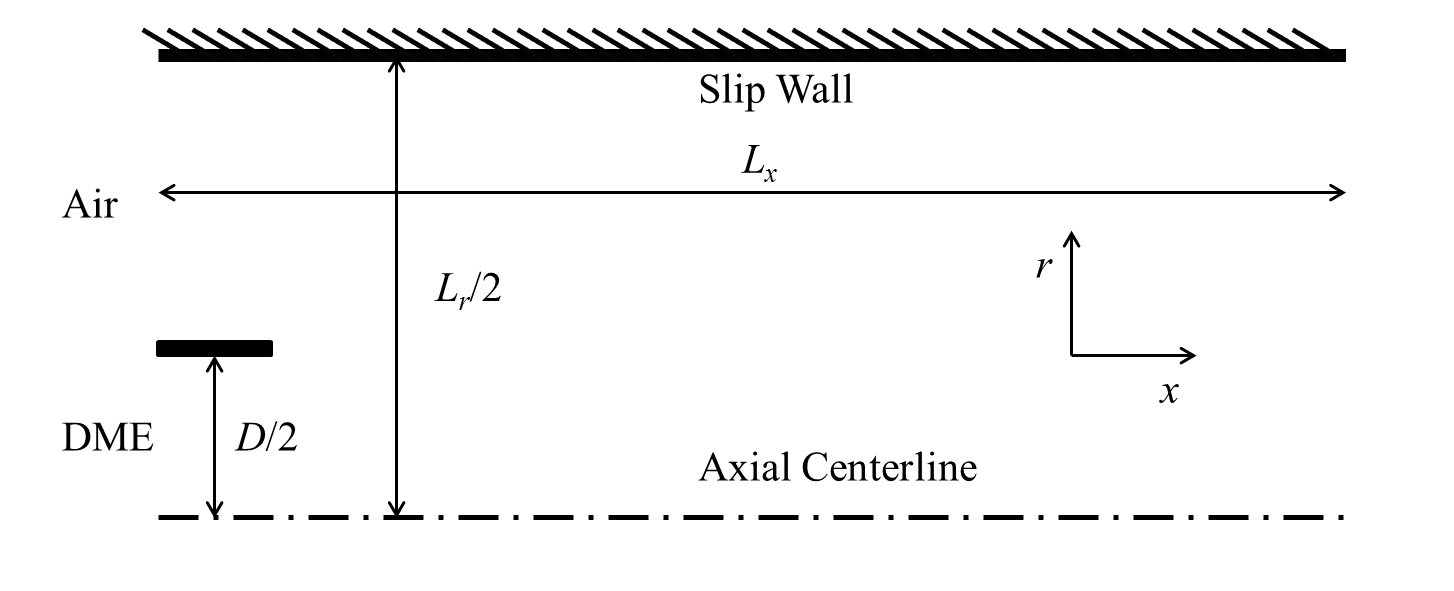
\includegraphics[width=1.0\textwidth]{ch-dynamics/coflow.png}
  \normalsize
  \caption{A schematic of the coflow configuration adopted in all of the steady and unsteady cases.}
  \label{fig:coflow}
\end{figure}

The flow field was initialized on a coarse mesh within a large domain.  At first, all the chemical source terms were set to zero until the nonreacting flow reached steady-state.  Chemical source terms were then activated; the mixture autoignited; and the flow field reached steady-state.  The domain was then truncated, and the mesh was refined to fully resolve the chemical structure.  All the results presented in Secs.~\ref{sec:dynamics-T} and~\ref{sec:dynamics-V} were obtained from the steady-state solutions.  

The Navier-Stokes equation with buoyancy in the streamwise direction and the conservation equations of mass, species, and temperature were solved.  The species diffusivities were determined from a constant, nonunity Lewis number.  The Lewis numbers for individual species were pre-calculated from a one-dimensional flamelet with the same boundary conditions and the mixture-averaged transport model and evaluated at the maximum temperature location.  The conserved scalar mixture fraction $Z$ was specified as unity and zero for the fuel jet and coflow at the inlet, respectively, and computed by solving its transport equation with unity Lewis number~\cite{pitsch98b}.  This definition of mixture fraction is consistent with the one used in the flamelet calculation in Sec.~\ref{sec:LFA}.

Dimethyl ether was chosen in this work, for it is a clean biofuel and one of the smallest hydrocarbons exhibiting NTC behavior.  The same skeletal mechanism~\cite{bhagatwala15} is utilized as in Chapter~\ref{ch:NTC}.

The low-Mach number formulation of the governing equations is solved using NGA, which is based on the numerical methods of Desjardins \emph{et al.}~\cite{desjardins08}.  The momentum and scalar equations are discretized with a second-order centered scheme and a third-order WENO scheme~\cite{liu94}, respectively, on a staggered mesh.  The iterative second-order semi-implicit Crank-Nicolson scheme of Pierce and Moin~\cite{pierce01} is adopted for temporal integration.  At each time step, the chemical source terms for the species and energy equations are evaluated independently from the transport terms using the CVODE package~\cite{cohen96}.

Uniform grids in the axial direction were adopted for the computations, and the grid spacing was set as $\Delta x = 2.2$ $\mu$m.  A nonuniform grid was used in the radial direction with a minimum spacing of $2.5$ $\mu$m to resolve the mixing layer corresponding to the separation wall and geometric progression stretch rates less than $3$\% towards both the centerline and the outer boundary.  The dimensions of and number of grid points in the computational domain for each computation are introduced in the following sections.

A grid convergence study was performed for the air temperature $800$ K case at $3.2$ m/s, for it has the most complex structure, which is discussed in the following sections.  As shown in Fig.~\ref{fig:convergence}, grid convergence was achieved for velocity, temperature, and species profiles.  Grid convergence was also verified for the air temperature $1100$ K case, which shows similar results and is therefore not shown here.  

\begin{figure}
  \centering
  \scriptsize
  \scalebox{1.5}{% GNUPLOT: LaTeX picture with Postscript
\begingroup
  \makeatletter
  \providecommand\color[2][]{%
    \GenericError{(gnuplot) \space\space\space\@spaces}{%
      Package color not loaded in conjunction with
      terminal option `colourtext'%
    }{See the gnuplot documentation for explanation.%
    }{Either use 'blacktext' in gnuplot or load the package
      color.sty in LaTeX.}%
    \renewcommand\color[2][]{}%
  }%
  \providecommand\includegraphics[2][]{%
    \GenericError{(gnuplot) \space\space\space\@spaces}{%
      Package graphicx or graphics not loaded%
    }{See the gnuplot documentation for explanation.%
    }{The gnuplot epslatex terminal needs graphicx.sty or graphics.sty.}%
    \renewcommand\includegraphics[2][]{}%
  }%
  \providecommand\rotatebox[2]{#2}%
  \@ifundefined{ifGPcolor}{%
    \newif\ifGPcolor
    \GPcolortrue
  }{}%
  \@ifundefined{ifGPblacktext}{%
    \newif\ifGPblacktext
    \GPblacktexttrue
  }{}%
  % define a \g@addto@macro without @ in the name:
  \let\gplgaddtomacro\g@addto@macro
  % define empty templates for all commands taking text:
  \gdef\gplbacktext{}%
  \gdef\gplfronttext{}%
  \makeatother
  \ifGPblacktext
    % no textcolor at all
    \def\colorrgb#1{}%
    \def\colorgray#1{}%
  \else
    % gray or color?
    \ifGPcolor
      \def\colorrgb#1{\color[rgb]{#1}}%
      \def\colorgray#1{\color[gray]{#1}}%
      \expandafter\def\csname LTw\endcsname{\color{white}}%
      \expandafter\def\csname LTb\endcsname{\color{black}}%
      \expandafter\def\csname LTa\endcsname{\color{black}}%
      \expandafter\def\csname LT0\endcsname{\color[rgb]{1,0,0}}%
      \expandafter\def\csname LT1\endcsname{\color[rgb]{0,1,0}}%
      \expandafter\def\csname LT2\endcsname{\color[rgb]{0,0,1}}%
      \expandafter\def\csname LT3\endcsname{\color[rgb]{1,0,1}}%
      \expandafter\def\csname LT4\endcsname{\color[rgb]{0,1,1}}%
      \expandafter\def\csname LT5\endcsname{\color[rgb]{1,1,0}}%
      \expandafter\def\csname LT6\endcsname{\color[rgb]{0,0,0}}%
      \expandafter\def\csname LT7\endcsname{\color[rgb]{1,0.3,0}}%
      \expandafter\def\csname LT8\endcsname{\color[rgb]{0.5,0.5,0.5}}%
    \else
      % gray
      \def\colorrgb#1{\color{black}}%
      \def\colorgray#1{\color[gray]{#1}}%
      \expandafter\def\csname LTw\endcsname{\color{white}}%
      \expandafter\def\csname LTb\endcsname{\color{black}}%
      \expandafter\def\csname LTa\endcsname{\color{black}}%
      \expandafter\def\csname LT0\endcsname{\color{black}}%
      \expandafter\def\csname LT1\endcsname{\color{black}}%
      \expandafter\def\csname LT2\endcsname{\color{black}}%
      \expandafter\def\csname LT3\endcsname{\color{black}}%
      \expandafter\def\csname LT4\endcsname{\color{black}}%
      \expandafter\def\csname LT5\endcsname{\color{black}}%
      \expandafter\def\csname LT6\endcsname{\color{black}}%
      \expandafter\def\csname LT7\endcsname{\color{black}}%
      \expandafter\def\csname LT8\endcsname{\color{black}}%
    \fi
  \fi
  \setlength{\unitlength}{0.0500bp}%
  \begin{picture}(3240.00,2520.00)%
    \gplgaddtomacro\gplbacktext{%
      \csname LTb\endcsname%
      \put(682,704){\makebox(0,0)[r]{\strut{} 0}}%
      \put(682,1092){\makebox(0,0)[r]{\strut{} 1}}%
      \put(682,1480){\makebox(0,0)[r]{\strut{} 2}}%
      \put(682,1868){\makebox(0,0)[r]{\strut{} 3}}%
      \put(682,2256){\makebox(0,0)[r]{\strut{} 4}}%
      \put(814,484){\makebox(0,0){\strut{} 0}}%
      \put(1220,484){\makebox(0,0){\strut{} 2}}%
      \put(1626,484){\makebox(0,0){\strut{} 4}}%
      \put(2031,484){\makebox(0,0){\strut{} 6}}%
      \put(2437,484){\makebox(0,0){\strut{} 8}}%
      \put(2843,484){\makebox(0,0){\strut{} 10}}%
      \put(176,1480){\rotatebox{-270}{\makebox(0,0){\strut{}\vspace{-28pt}$U$ [m/s]}}}%
      \put(1828,154){\makebox(0,0){\strut{}$x/D$}}%
      \put(1475,1170){\makebox(0,0)[l]{\strut{}Nominal}}%
      \put(1475,956){\makebox(0,0)[l]{\strut{}Coarser}}%
    }%
    \gplgaddtomacro\gplfronttext{%
      \csname LTb\endcsname%
      \put(2003,1176){\makebox(0,0)[r]{\strut{} }}%
      \csname LTb\endcsname%
      \put(2003,956){\makebox(0,0)[r]{\strut{} }}%
    }%
    \gplbacktext
    \put(0,0){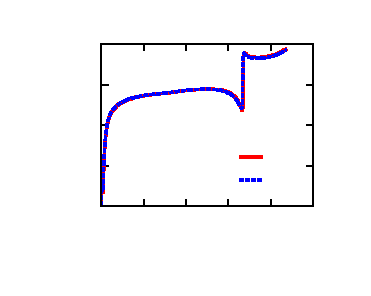
\includegraphics{ch-dynamics/conv_zst_U}}%
    \gplfronttext
  \end{picture}%
\endgroup
}
  \scalebox{1.5}{% GNUPLOT: LaTeX picture with Postscript
\begingroup
  \makeatletter
  \providecommand\color[2][]{%
    \GenericError{(gnuplot) \space\space\space\@spaces}{%
      Package color not loaded in conjunction with
      terminal option `colourtext'%
    }{See the gnuplot documentation for explanation.%
    }{Either use 'blacktext' in gnuplot or load the package
      color.sty in LaTeX.}%
    \renewcommand\color[2][]{}%
  }%
  \providecommand\includegraphics[2][]{%
    \GenericError{(gnuplot) \space\space\space\@spaces}{%
      Package graphicx or graphics not loaded%
    }{See the gnuplot documentation for explanation.%
    }{The gnuplot epslatex terminal needs graphicx.sty or graphics.sty.}%
    \renewcommand\includegraphics[2][]{}%
  }%
  \providecommand\rotatebox[2]{#2}%
  \@ifundefined{ifGPcolor}{%
    \newif\ifGPcolor
    \GPcolortrue
  }{}%
  \@ifundefined{ifGPblacktext}{%
    \newif\ifGPblacktext
    \GPblacktexttrue
  }{}%
  % define a \g@addto@macro without @ in the name:
  \let\gplgaddtomacro\g@addto@macro
  % define empty templates for all commands taking text:
  \gdef\gplbacktext{}%
  \gdef\gplfronttext{}%
  \makeatother
  \ifGPblacktext
    % no textcolor at all
    \def\colorrgb#1{}%
    \def\colorgray#1{}%
  \else
    % gray or color?
    \ifGPcolor
      \def\colorrgb#1{\color[rgb]{#1}}%
      \def\colorgray#1{\color[gray]{#1}}%
      \expandafter\def\csname LTw\endcsname{\color{white}}%
      \expandafter\def\csname LTb\endcsname{\color{black}}%
      \expandafter\def\csname LTa\endcsname{\color{black}}%
      \expandafter\def\csname LT0\endcsname{\color[rgb]{1,0,0}}%
      \expandafter\def\csname LT1\endcsname{\color[rgb]{0,1,0}}%
      \expandafter\def\csname LT2\endcsname{\color[rgb]{0,0,1}}%
      \expandafter\def\csname LT3\endcsname{\color[rgb]{1,0,1}}%
      \expandafter\def\csname LT4\endcsname{\color[rgb]{0,1,1}}%
      \expandafter\def\csname LT5\endcsname{\color[rgb]{1,1,0}}%
      \expandafter\def\csname LT6\endcsname{\color[rgb]{0,0,0}}%
      \expandafter\def\csname LT7\endcsname{\color[rgb]{1,0.3,0}}%
      \expandafter\def\csname LT8\endcsname{\color[rgb]{0.5,0.5,0.5}}%
    \else
      % gray
      \def\colorrgb#1{\color{black}}%
      \def\colorgray#1{\color[gray]{#1}}%
      \expandafter\def\csname LTw\endcsname{\color{white}}%
      \expandafter\def\csname LTb\endcsname{\color{black}}%
      \expandafter\def\csname LTa\endcsname{\color{black}}%
      \expandafter\def\csname LT0\endcsname{\color{black}}%
      \expandafter\def\csname LT1\endcsname{\color{black}}%
      \expandafter\def\csname LT2\endcsname{\color{black}}%
      \expandafter\def\csname LT3\endcsname{\color{black}}%
      \expandafter\def\csname LT4\endcsname{\color{black}}%
      \expandafter\def\csname LT5\endcsname{\color{black}}%
      \expandafter\def\csname LT6\endcsname{\color{black}}%
      \expandafter\def\csname LT7\endcsname{\color{black}}%
      \expandafter\def\csname LT8\endcsname{\color{black}}%
    \fi
  \fi
  \setlength{\unitlength}{0.0500bp}%
  \begin{picture}(3600.00,2520.00)%
    \gplgaddtomacro\gplbacktext{%
      \csname LTb\endcsname%
      \put(1078,704){\makebox(0,0)[r]{\strut{} 600}}%
      \put(1078,1014){\makebox(0,0)[r]{\strut{} 1000}}%
      \put(1078,1325){\makebox(0,0)[r]{\strut{} 1400}}%
      \put(1078,1635){\makebox(0,0)[r]{\strut{} 1800}}%
      \put(1078,1946){\makebox(0,0)[r]{\strut{} 2200}}%
      \put(1078,2256){\makebox(0,0)[r]{\strut{} 2600}}%
      \put(1210,484){\makebox(0,0){\strut{} 0}}%
      \put(1609,484){\makebox(0,0){\strut{} 2}}%
      \put(2007,484){\makebox(0,0){\strut{} 4}}%
      \put(2406,484){\makebox(0,0){\strut{} 6}}%
      \put(2804,484){\makebox(0,0){\strut{} 8}}%
      \put(3203,484){\makebox(0,0){\strut{} 10}}%
      \put(176,1480){\rotatebox{-270}{\makebox(0,0){\strut{}\vspace{-48pt}$T$ [K]}}}%
      \put(2206,154){\makebox(0,0){\strut{}$x/D$}}%
      \put(1459,2023){\makebox(0,0)[l]{\strut{}Nominal}}%
      \put(1459,1790){\makebox(0,0)[l]{\strut{}Coarser}}%
    }%
    \gplgaddtomacro\gplfronttext{%
      \csname LTb\endcsname%
      \put(1871,2037){\makebox(0,0)[r]{\strut{} }}%
      \csname LTb\endcsname%
      \put(1871,1817){\makebox(0,0)[r]{\strut{} }}%
    }%
    \gplbacktext
    \put(0,0){
\includegraphics{conv_zst_T}}%
    \gplfronttext
  \end{picture}%
\endgroup
}
  \scalebox{1.5}{% GNUPLOT: LaTeX picture with Postscript
\begingroup
  \makeatletter
  \providecommand\color[2][]{%
    \GenericError{(gnuplot) \space\space\space\@spaces}{%
      Package color not loaded in conjunction with
      terminal option `colourtext'%
    }{See the gnuplot documentation for explanation.%
    }{Either use 'blacktext' in gnuplot or load the package
      color.sty in LaTeX.}%
    \renewcommand\color[2][]{}%
  }%
  \providecommand\includegraphics[2][]{%
    \GenericError{(gnuplot) \space\space\space\@spaces}{%
      Package graphicx or graphics not loaded%
    }{See the gnuplot documentation for explanation.%
    }{The gnuplot epslatex terminal needs graphicx.sty or graphics.sty.}%
    \renewcommand\includegraphics[2][]{}%
  }%
  \providecommand\rotatebox[2]{#2}%
  \@ifundefined{ifGPcolor}{%
    \newif\ifGPcolor
    \GPcolortrue
  }{}%
  \@ifundefined{ifGPblacktext}{%
    \newif\ifGPblacktext
    \GPblacktexttrue
  }{}%
  % define a \g@addto@macro without @ in the name:
  \let\gplgaddtomacro\g@addto@macro
  % define empty templates for all commands taking text:
  \gdef\gplbacktext{}%
  \gdef\gplfronttext{}%
  \makeatother
  \ifGPblacktext
    % no textcolor at all
    \def\colorrgb#1{}%
    \def\colorgray#1{}%
  \else
    % gray or color?
    \ifGPcolor
      \def\colorrgb#1{\color[rgb]{#1}}%
      \def\colorgray#1{\color[gray]{#1}}%
      \expandafter\def\csname LTw\endcsname{\color{white}}%
      \expandafter\def\csname LTb\endcsname{\color{black}}%
      \expandafter\def\csname LTa\endcsname{\color{black}}%
      \expandafter\def\csname LT0\endcsname{\color[rgb]{1,0,0}}%
      \expandafter\def\csname LT1\endcsname{\color[rgb]{0,1,0}}%
      \expandafter\def\csname LT2\endcsname{\color[rgb]{0,0,1}}%
      \expandafter\def\csname LT3\endcsname{\color[rgb]{1,0,1}}%
      \expandafter\def\csname LT4\endcsname{\color[rgb]{0,1,1}}%
      \expandafter\def\csname LT5\endcsname{\color[rgb]{1,1,0}}%
      \expandafter\def\csname LT6\endcsname{\color[rgb]{0,0,0}}%
      \expandafter\def\csname LT7\endcsname{\color[rgb]{1,0.3,0}}%
      \expandafter\def\csname LT8\endcsname{\color[rgb]{0.5,0.5,0.5}}%
    \else
      % gray
      \def\colorrgb#1{\color{black}}%
      \def\colorgray#1{\color[gray]{#1}}%
      \expandafter\def\csname LTw\endcsname{\color{white}}%
      \expandafter\def\csname LTb\endcsname{\color{black}}%
      \expandafter\def\csname LTa\endcsname{\color{black}}%
      \expandafter\def\csname LT0\endcsname{\color{black}}%
      \expandafter\def\csname LT1\endcsname{\color{black}}%
      \expandafter\def\csname LT2\endcsname{\color{black}}%
      \expandafter\def\csname LT3\endcsname{\color{black}}%
      \expandafter\def\csname LT4\endcsname{\color{black}}%
      \expandafter\def\csname LT5\endcsname{\color{black}}%
      \expandafter\def\csname LT6\endcsname{\color{black}}%
      \expandafter\def\csname LT7\endcsname{\color{black}}%
      \expandafter\def\csname LT8\endcsname{\color{black}}%
    \fi
  \fi
  \setlength{\unitlength}{0.0500bp}%
  \begin{picture}(3744.00,2520.00)%
    \gplgaddtomacro\gplbacktext{%
      \csname LTb\endcsname%
      \put(1210,704){\makebox(0,0)[r]{\strut{} 0}}%
      \put(1210,1014){\makebox(0,0)[r]{\strut{} 0.002}}%
      \put(1210,1325){\makebox(0,0)[r]{\strut{} 0.004}}%
      \put(1210,1635){\makebox(0,0)[r]{\strut{} 0.006}}%
      \put(1210,1946){\makebox(0,0)[r]{\strut{} 0.008}}%
      \put(1210,2256){\makebox(0,0)[r]{\strut{} 0.01}}%
      \put(1342,484){\makebox(0,0){\strut{} 0}}%
      \put(1743,484){\makebox(0,0){\strut{} 2}}%
      \put(2144,484){\makebox(0,0){\strut{} 4}}%
      \put(2545,484){\makebox(0,0){\strut{} 6}}%
      \put(2946,484){\makebox(0,0){\strut{} 8}}%
      \put(3347,484){\makebox(0,0){\strut{} 10}}%
      \put(176,1480){\rotatebox{-270}{\makebox(0,0){\strut{}\vspace{-52pt}$Y_{\rm H_2O_2}$}}}%
      \put(2344,154){\makebox(0,0){\strut{}$x/D$}}%
      \put(1593,2023){\makebox(0,0)[l]{\strut{}Nominal}}%
      \put(1593,1790){\makebox(0,0)[l]{\strut{}Coarser}}%
    }%
    \gplgaddtomacro\gplfronttext{%
      \csname LTb\endcsname%
      \put(2035,2022){\makebox(0,0)[r]{\strut{} }}%
      \csname LTb\endcsname%
      \put(2035,1802){\makebox(0,0)[r]{\strut{} }}%
    }%
    \gplbacktext
    \put(0,0){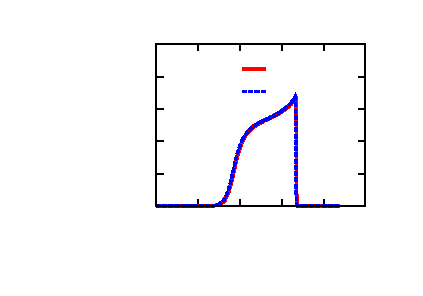
\includegraphics{conv_zst_H2O2}}%
    \gplfronttext
  \end{picture}%
\endgroup
}
  \caption{Velocity, temperature, and H$_2$O$_2$ profiles along $Z_{\rm st}$ on the nominal and two times coarser (in each direction) meshes for an air temperature of $800$ K.}
  \label{fig:convergence}
\end{figure}

\section{Flame Stabilization: Boundary Temperature Effects}\label{sec:dynamics-T}

In this section, the effect of boundary temperature on flame stabilization is investigated.  Therefore, in all cases studied in this section, the boundary velocities of the DME jet as well as the coflow air are fixed at $3.2$ m/s.  Conversely, the temperatures of the heated air coflow are $700$, $800$, $900$, and $1100$ K.  The dimensions of and number of grid points in the computational domain for each computation are summarized in Table~\ref{table:domain_T}. 

\begin{table*}
  \caption{Computational domain and number of grid points for steady cases with the same flow velocities but different boundary temperatures.}
  \label{table:domain_T}
  \centering
  \normalsize
  \resizebox{0.8\textwidth}{!}{
  \begin{tabular}{lc*{3}{c}}
    \hline
    Coflow Temperature [K]& $700$  & $800$  & $900$  & $1100$   \\
    \hline
    $L_x$ [mm]& $28$ & $7$ & $3.5$ & $3$\\
    $L_r$ [mm]& $6$ & $3.9$ & $3.9$  & $6$\\
    $N_x$ & $12290$ & $3072$ & $1536$  & $1282$\\
    $N_r$ & $192$ & $176$ & $176$  & $192$\\
    \hline
   \end{tabular}
}
\end{table*}

\subsection{Thermal and Chemical Structure} \label{sec:dynamcis-structure_T}

To visualize the flame structures, the heat release rate profiles for the four cases ($700$, $800$, $900$, and $1100$ K) are shown in Fig.~\ref{fig:dynamics-HRR_T}.  Qualitatively, the most upstream point on the largest heat release contour (the leading point), colored by red, will be referred to as the stabilization point.  

\begin{figure}[t]
  \centering
  \scriptsize
  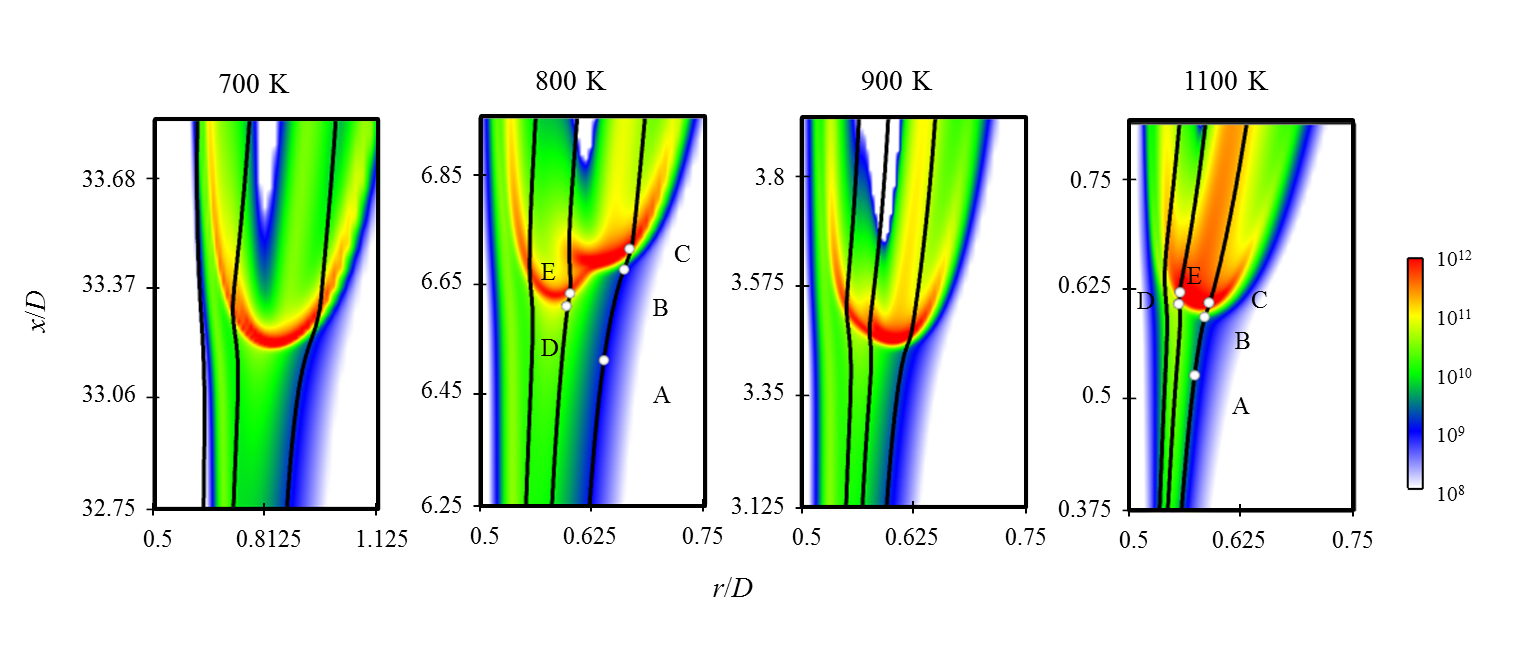
\includegraphics[width=1.0\textwidth]{ch-dynamics/HRR_T.png}
  \normalsize
  \caption{Heat release rate [J/m$^3$-s] profiles for the steady cases with the same flow velocities but different boundary temperatures.  The iso-contours of $Z_{\rm st}$, $Z = 0.2$, and $Z = 0.3$ are outlined from right to left in solid lines, respectively.  The CEMA sampling points at $800$ and $1100$ K are indicated along the iso-contours.}
  \label{fig:dynamics-HRR_T}
\end{figure}

At $700$ K, a tribrachial thermal structure is observed, and the stabilization point is located around $Z = 0.15$, which is richer than the triple point, where the three branches intersect.  Moreover, compared to the classical triple flame structure, the middle heat release rate branch, corresponding to the nonpremixed flame, is significantly weaker than the other two branches.  

At $800$ K, the stabilization point is not located on the tribrachial structure any more.  Instead, it is located near $Z = 0.23$ and connects two trailing heat release branches, where a tribrachial flame structure is attached to the leaner branch (LB) of the bibrachial reacting front.  A schematic of the structure is shown in Fig.~\ref{fig:schematic_800}.

\begin{figure}[t]
  \centering
  \scriptsize
  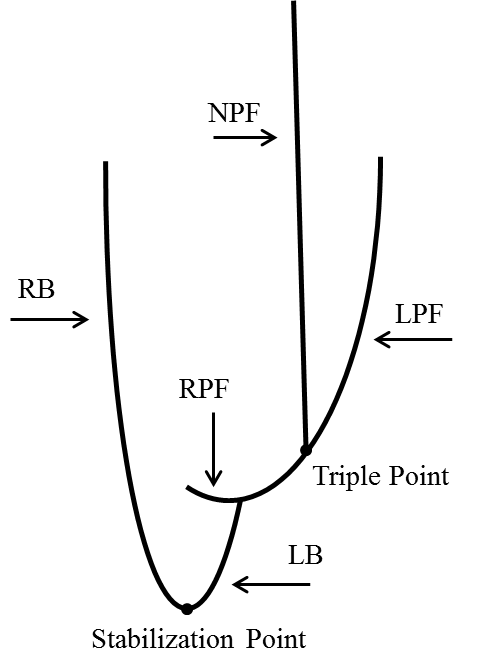
\includegraphics[width=0.4\textwidth]{ch-dynamics/schematic_800.png}
  \normalsize
  \caption{A schematic of the thermal structure of the $800$ K case.  LPF, RPF, and NPF denotes the lean premixed, rich premixed, and nonpremixed flame branches on the tribrachial structure, respectively.  LB and RB denotes the leaner and richer branches of the reacting front, respectively.}
  \label{fig:schematic_800}
\end{figure}

As the air boundary temperature increases to $900$ K, the stabilization point shifts back to $Z = 0.14$.  Moreover, a long trailing branch at richer mixture fraction is attached to the main tribrachial structure, resulting in a tetrabrachial structure.  Compared with the structure shown in the $800$ K case, the main tribrachial structure stabilizes further upstream, for it depends less on the radical accumulation ahead of the flame.  Therefore, it catches up with the reacting front at richer mixture fraction, and they merge into the apparent tetrabrachial structure.

A further increase in the boundary temperature results in a structure that is very similar to the classical triple flame, except for the fact that there is also heat release ahead of the stabilization point at $Z = 0.13$.  Some of the multibrachial structures were also observed by Krisman \emph{et al.}~\cite{krisman15}, using different definitions for branches, and it was concluded that the autoignition chemistry could affect the flame structure and the stabilization mechanism.  

To first qualitatively demonstrate the chemical structure of the flame, selected species profiles were examined, shown in Figs.~\ref{fig:OH_T} to~\ref{fig:H2O2_T}.  The methoxymethylperoxy radical (CH$_3$OCH$_2$O$_2$) and hydroxyl radical (OH) were chosen as indicators of low and high-temperature chemistry, respectively.  The hydroperoxyl radical (HO$_2$) and hydrogen peroxide (H$_2$O$_2$) were chosen, for they form in the preheat zone of a flame or before autoignition but quickly vanish in the post flame zone or after ignition~\cite{yoo09}.

For all four cases, similar profiles can be seen for some species.  First, low-temperature chemistry, indicated by the CH$_3$OCH$_2$O$_2$ radical, is found to be important at richer mixture fractions, where the temperature is also lower.  Second, the OH radical peaks at and downstream of the maximum heat release locations and correlates well with the tribrachial structure shown in the heat release rate profiles, indicating the presence of high-temperature chemistry.  Third, the HO$_2$ mass fraction peaks in a thin region.  Compared with the heat release rate contours, this thin region outlines the flame front and the reactive mixture at the rich mixture fractions and indicates the importance of the exothermic three-body recombination reaction H + O$_2$ + M $\Longleftrightarrow$ HO$_2$ + M.

However, there are also differences in the chemical structure among the different cases.  For example, for the $800$ and $900$ K cases, another OH local maxima, which is two orders of magnitudes smaller than the peak value on the tribrachial structure, appears at richer mixture fractions, immediately downstream of where the CH$_3$OCH$_2$O$_2$ radical and H$_2$O$_2$ disappear, indicating autoignition.  Moreover, more pronounced differences between the three lower boundary temperature cases and the $1100$ K case are shown in the H$_2$O$_2$ profiles: for the lower boundary temperature cases, H$_2$O$_2$ accumulates along the mixture fraction iso-contours  until it decomposes in the flame region, while, for the $1100$ K case, the H$_2$O$_2$ accumulation is an order of magnitude lower, due to the reduced residence time from the nozzle exit to the flame base.

\begin{figure}[t]
  \centering
  \scriptsize
  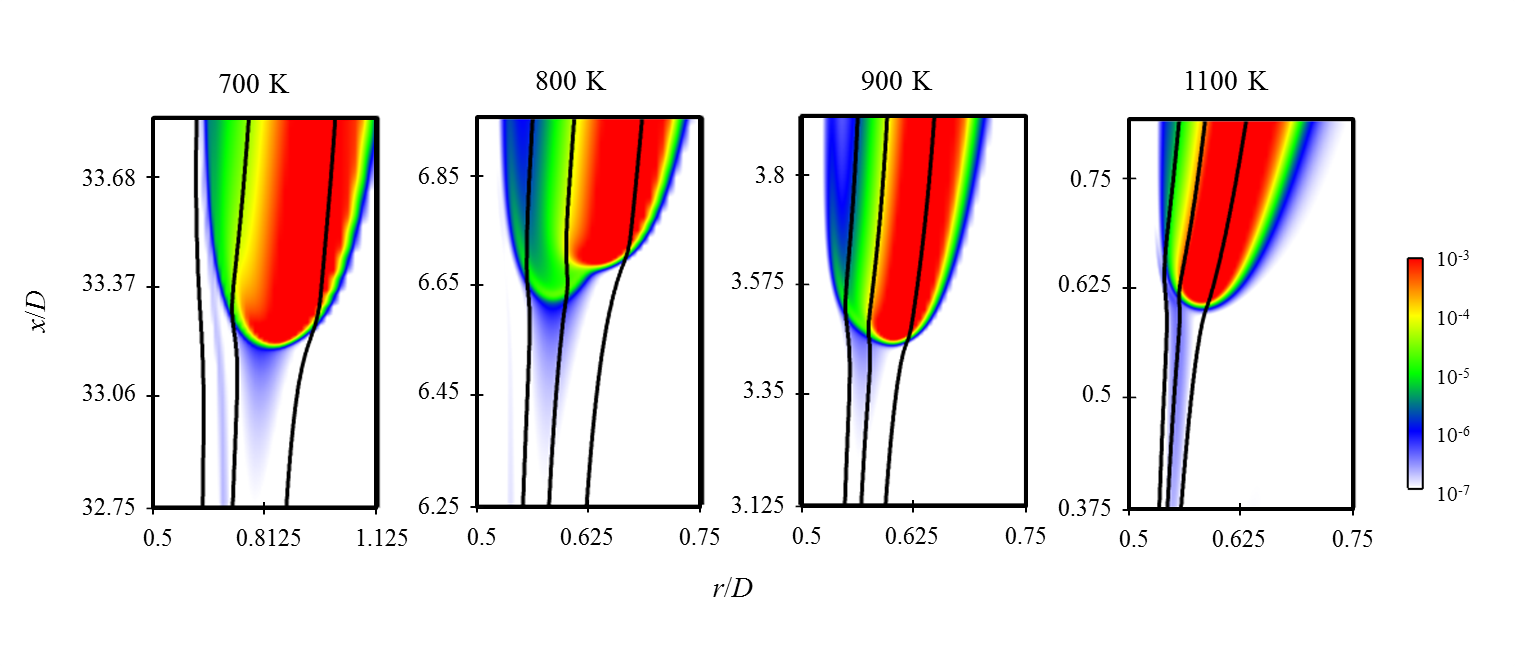
\includegraphics[width=1.0\textwidth]{ch-dynamics/OH_T.png}
  \normalsize
  \caption{Hydroxyl (OH) radical mass fraction profiles for the steady cases with the same flow velocities but different boundary temperatures.  The mixture fraction iso-contours are the same as in Fig.~\ref{fig:dynamics-HRR_T}.}
  \label{fig:OH_T}
\end{figure}

\begin{figure}[t]
  \centering
  \scriptsize
  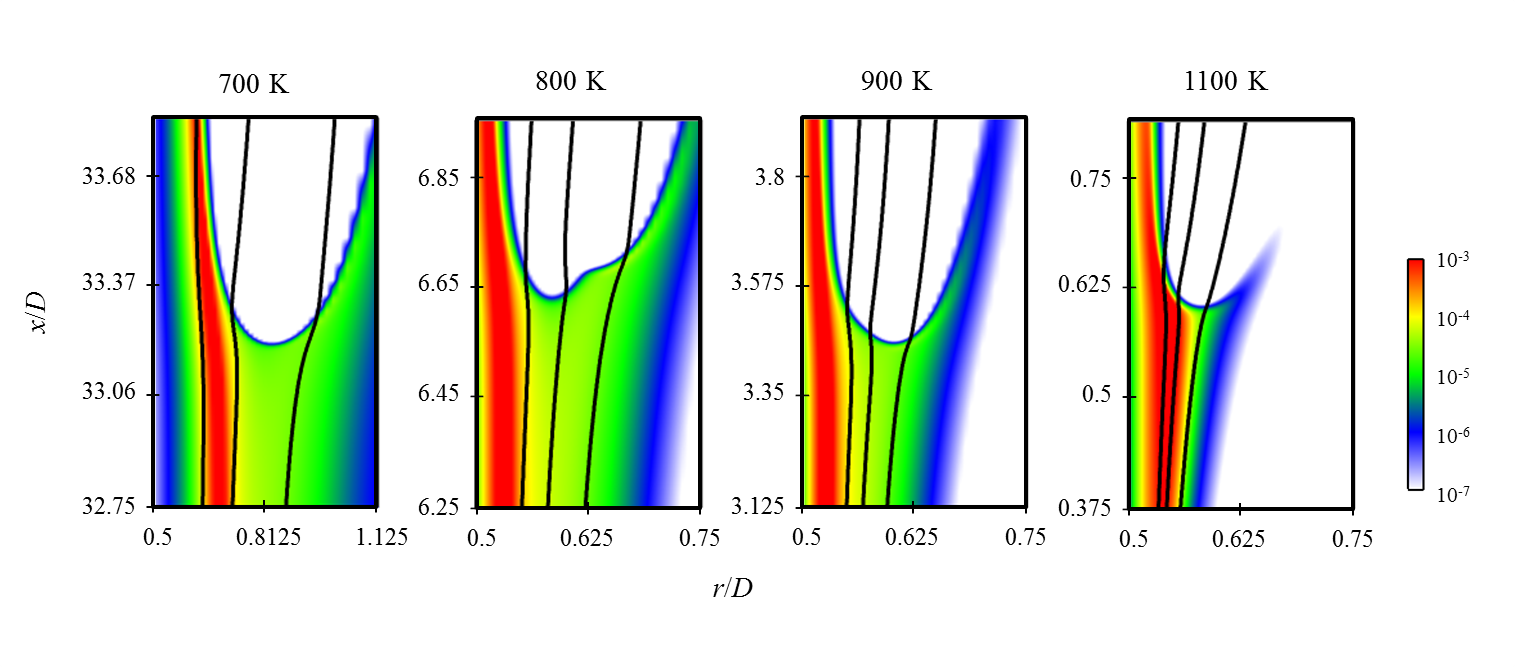
\includegraphics[width=1.0\textwidth]{ch-dynamics/RO2_T.png}
  \normalsize
  \caption{Methoxymethylperoxy (CH$_3$OCH$_2$O$_2$) radical mass fraction profiles for the steady cases with the same flow velocities but different boundary temperatures.  The mixture fraction iso-contours are the same as in Fig.~\ref{fig:dynamics-HRR_T}.}
  \label{fig:RO2_T}
\end{figure}

\begin{figure}[t]
  \centering
  \scriptsize
  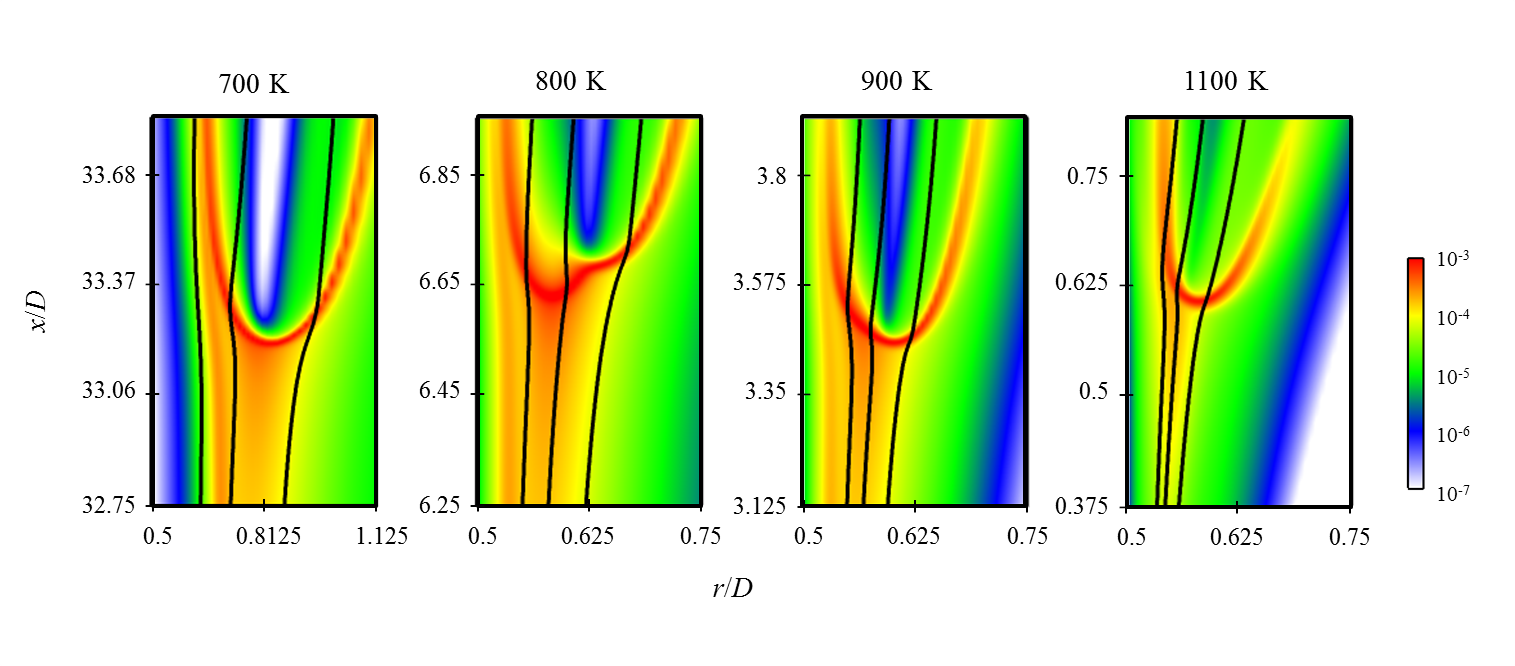
\includegraphics[width=1.0\textwidth]{ch-dynamics/HO2_T.png}
  \normalsize
  \caption{Hydroperoxyl (HO$_2$) radical mass fraction profiles for the steady cases with the same flow velocities but different boundary temperatures.  The mixture fraction iso-contours are the same as in Fig.~\ref{fig:dynamics-HRR_T}.}
  \label{fig:HO2_T}
\end{figure}

\begin{figure}[t]
  \centering
  \scriptsize
  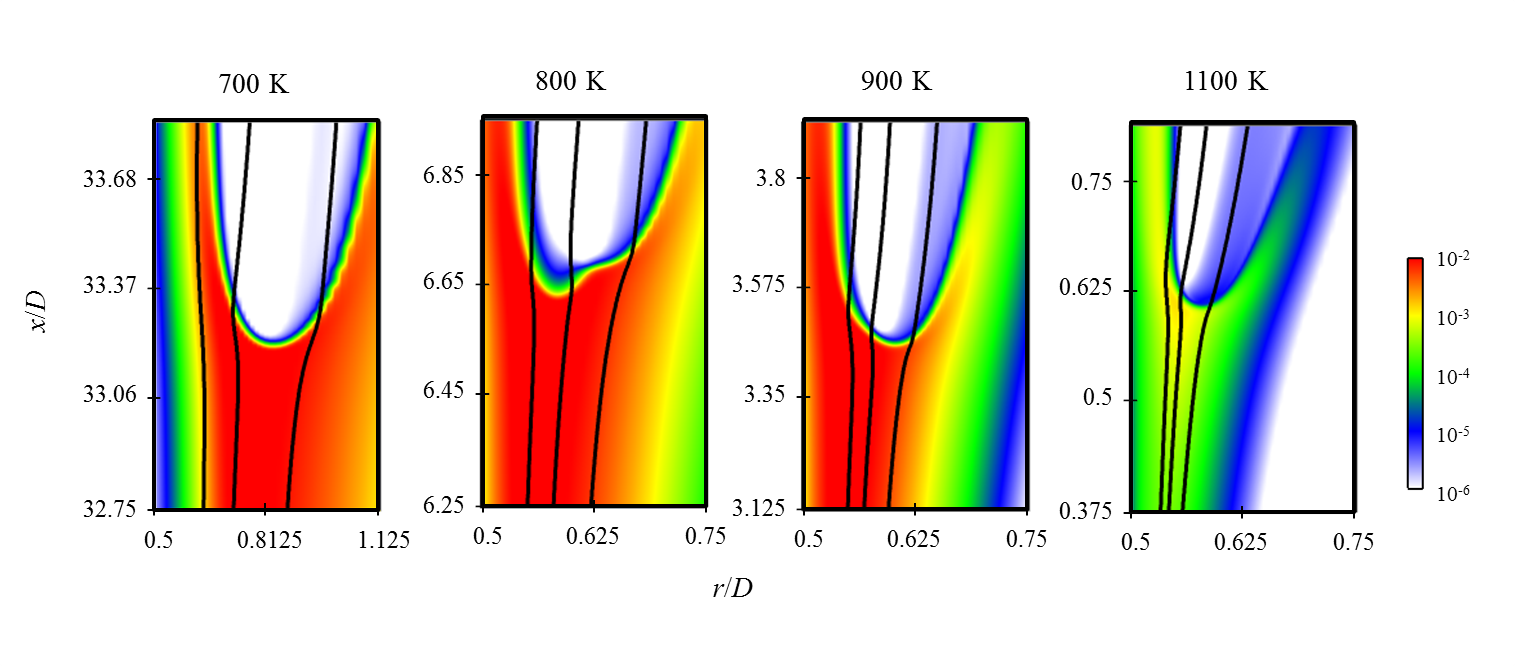
\includegraphics[width=1.0\textwidth]{ch-dynamics/H2O2_T.png}
  \normalsize
  \caption{Hydrogen peroxide (H$_2$O$_2$) mass fraction profiles for the steady cases with the same flow velocities but different boundary temperatures.  The mixture fraction iso-contours are the same as in Fig.~\ref{fig:dynamics-HRR_T}.}
  \label{fig:H2O2_T}
\end{figure}

\subsection{Computational Diagnostics and Analysis} \label{sec:diagnostics}

The above heat release rate and species profiles demonstrate the thermal and chemical structure of the reacting fronts at different boundary temperatures.  However, more detailed computational diagnostics and analysis are needed to further demonstrate the controlling chemistry and the stabilization mechanism.

\subsubsection{Chemical Explosive Mode Analysis}
In addition to the analysis based on selected species profiles, Chemical Explosive Mode Analysis (CEMA)~\cite{lu10,shan12} was conducted to identify the controlling chemistry in these complex reacting flows.  Briefly, local species concentrations and temperature are sampled from the two-dimensional computation and input into CEMA to evaluate the eigenvalues of the Jacobian matrix ($K + 1$ by $K + 1$, where $K$ is the number of species) of the chemical source terms.  The eigenmode associated with the eigenvalue $\lambda_{\rm e}$, which has the largest real part among all the eigenvalues, is defined as a chemical explosive mode, if

\begin{equation}
\rm{Re}(\lambda_{\rm e}) > 0, \lambda_{\rm e} = \mathbf{b_{\rm e}J_{\omega}a_{\rm e}},
\end{equation}
where $\mathbf{b_{\rm e}}$ and $\mathbf{a_{\rm e}}$ are the left and right eigenvectors, respectively, associated with $\lambda_{\rm e}$, and $\mathbf{J_{\omega}}$ is the chemical Jacobian matrix.  The existence of the chemical explosive mode indicates the propensity of local mixture autoignition given an isolated, adiabatic, and constant volume environment.  Furthermore, the detailed chemical reactions that contribute to the chemical explosive mode can be quantified by the explosion participation index:

\begin{equation}
\mathbf{PI} = \frac{|(\mathbf{b_{\rm e}} \cdot \mathbf{S}) \otimes \mathbf{R}|}{sum(|(\mathbf{b_{\rm e}} \cdot \mathbf{S}) \otimes \mathbf{R}|)},
\end{equation}
where $\mathbf{S}$ is the stoichiometric coefficient matrix, $\mathbf{R}$ is the vector of the net rates for the reactions, and $\otimes$ denotes elementwise multiplication of two vectors.  

The dominant reactions at representative locations, such as those upstream and near the flame base, are identified, based on the explosive mode and participation index.  For each case, the local species concentrations and temperature were sampled along the $Z_{\rm st}$, $Z = 0.2$, and $Z = 0.3$ iso-contours, as indicated in Fig.~\ref{fig:dynamics-HRR_T}, and processed by CEMA to demonstrate the evolution of the dominant reactions.

\begin{figure}
  \centering
  \scriptsize
  % GNUPLOT: LaTeX picture with Postscript
\begingroup
  \makeatletter
  \providecommand\color[2][]{%
    \GenericError{(gnuplot) \space\space\space\@spaces}{%
      Package color not loaded in conjunction with
      terminal option `colourtext'%
    }{See the gnuplot documentation for explanation.%
    }{Either use 'blacktext' in gnuplot or load the package
      color.sty in LaTeX.}%
    \renewcommand\color[2][]{}%
  }%
  \providecommand\includegraphics[2][]{%
    \GenericError{(gnuplot) \space\space\space\@spaces}{%
      Package graphicx or graphics not loaded%
    }{See the gnuplot documentation for explanation.%
    }{The gnuplot epslatex terminal needs graphicx.sty or graphics.sty.}%
    \renewcommand\includegraphics[2][]{}%
  }%
  \providecommand\rotatebox[2]{#2}%
  \@ifundefined{ifGPcolor}{%
    \newif\ifGPcolor
    \GPcolortrue
  }{}%
  \@ifundefined{ifGPblacktext}{%
    \newif\ifGPblacktext
    \GPblacktexttrue
  }{}%
  % define a \g@addto@macro without @ in the name:
  \let\gplgaddtomacro\g@addto@macro
  % define empty templates for all commands taking text:
  \gdef\gplbacktext{}%
  \gdef\gplfronttext{}%
  \makeatother
  \ifGPblacktext
    % no textcolor at all
    \def\colorrgb#1{}%
    \def\colorgray#1{}%
  \else
    % gray or color?
    \ifGPcolor
      \def\colorrgb#1{\color[rgb]{#1}}%
      \def\colorgray#1{\color[gray]{#1}}%
      \expandafter\def\csname LTw\endcsname{\color{white}}%
      \expandafter\def\csname LTb\endcsname{\color{black}}%
      \expandafter\def\csname LTa\endcsname{\color{black}}%
      \expandafter\def\csname LT0\endcsname{\color[rgb]{1,0,0}}%
      \expandafter\def\csname LT1\endcsname{\color[rgb]{0,1,0}}%
      \expandafter\def\csname LT2\endcsname{\color[rgb]{0,0,1}}%
      \expandafter\def\csname LT3\endcsname{\color[rgb]{1,0,1}}%
      \expandafter\def\csname LT4\endcsname{\color[rgb]{0,1,1}}%
      \expandafter\def\csname LT5\endcsname{\color[rgb]{1,1,0}}%
      \expandafter\def\csname LT6\endcsname{\color[rgb]{0,0,0}}%
      \expandafter\def\csname LT7\endcsname{\color[rgb]{1,0.3,0}}%
      \expandafter\def\csname LT8\endcsname{\color[rgb]{0.5,0.5,0.5}}%
    \else
      % gray
      \def\colorrgb#1{\color{black}}%
      \def\colorgray#1{\color[gray]{#1}}%
      \expandafter\def\csname LTw\endcsname{\color{white}}%
      \expandafter\def\csname LTb\endcsname{\color{black}}%
      \expandafter\def\csname LTa\endcsname{\color{black}}%
      \expandafter\def\csname LT0\endcsname{\color{black}}%
      \expandafter\def\csname LT1\endcsname{\color{black}}%
      \expandafter\def\csname LT2\endcsname{\color{black}}%
      \expandafter\def\csname LT3\endcsname{\color{black}}%
      \expandafter\def\csname LT4\endcsname{\color{black}}%
      \expandafter\def\csname LT5\endcsname{\color{black}}%
      \expandafter\def\csname LT6\endcsname{\color{black}}%
      \expandafter\def\csname LT7\endcsname{\color{black}}%
      \expandafter\def\csname LT8\endcsname{\color{black}}%
    \fi
  \fi
  \setlength{\unitlength}{0.0500bp}%
  \begin{picture}(7200.00,5040.00)%
    \gplgaddtomacro\gplbacktext{%
      \csname LTb\endcsname%
      \put(2748,1043){\makebox(0,0)[r]{\strut{}H$_2$O$_2$+M$\Longleftrightarrow$OH+OH+M}}%
      \put(2748,1383){\makebox(0,0)[r]{\strut{}HCO+O$_2$$\Longleftrightarrow$CO+HO$_2$}}%
      \put(2748,1722){\makebox(0,0)[r]{\strut{}CH$_2$OCH$_2$O$_2$H$\Longleftrightarrow$OH+CH$_2$O+CH$_2$O}}%
      \put(2748,2061){\makebox(0,0)[r]{\strut{}CH$_2$O+OH$\Longleftrightarrow$HCO+H$_2$O}}%
      \put(2748,2400){\makebox(0,0)[r]{\strut{}CH$_3$OCH$_3$+HO$_2$$\Longleftrightarrow$CH$_3$OCH$_2$+H$_2$O$_2$}}%
      \put(2748,2740){\makebox(0,0)[r]{\strut{}CH$_3$OCH$_2$+O$_2$$\Longleftrightarrow$CH$_3$OCH$_2$O$_2$}}%
      \put(2748,3079){\makebox(0,0)[r]{\strut{}HO$_2$+HO$_2$$\Longleftrightarrow$H$_2$O$_2$+O$_2$}}%
      \put(2748,3418){\makebox(0,0)[r]{\strut{}CH$_3$OCH$_2$O$_2$$\Longleftrightarrow$CH$_2$OCH$_2$O$_2$H}}%
      \put(2748,3757){\makebox(0,0)[r]{\strut{}H+O$_2$+M$\Longleftrightarrow$HO$_2$+M}}%
      \put(2748,4097){\makebox(0,0)[r]{\strut{}CH$_2$O+HO$_2$$\Longleftrightarrow$HCO+H$_2$O$_2$}}%
      \put(2748,4436){\makebox(0,0)[r]{\strut{}H+O$_2$$\Longleftrightarrow$O+OH}}%
      \put(2880,484){\makebox(0,0){\strut{}-1}}%
      \put(3861,484){\makebox(0,0){\strut{}-0.5}}%
      \put(4842,484){\makebox(0,0){\strut{} 0}}%
      \put(5822,484){\makebox(0,0){\strut{} 0.5}}%
      \put(6803,484){\makebox(0,0){\strut{} 1}}%
      \csname LTb\endcsname%
      \put(4841,154){\makebox(0,0){\strut{}Normalized Participation Index}}%
      \put(5234,1332){\makebox(0,0)[l]{\strut{}Point A}}%
      \put(5234,1501){\makebox(0,0)[l]{\strut{}Point B}}%
      \put(5234,1688){\makebox(0,0)[l]{\strut{}Point C}}%
      \put(5234,1857){\makebox(0,0)[l]{\strut{}Point D}}%
      \put(5234,2027){\makebox(0,0)[l]{\strut{}Point E}}%
      \put(5234,2231){\makebox(0,0)[l]{\strut{}$800$ K}}%
    }%
    \gplgaddtomacro\gplfronttext{%
      \csname LTb\endcsname%
      \put(5690,1337){\makebox(0,0)[r]{\strut{} }}%
      \csname LTb\endcsname%
      \put(5690,1513){\makebox(0,0)[r]{\strut{} }}%
      \csname LTb\endcsname%
      \put(5690,1689){\makebox(0,0)[r]{\strut{} }}%
      \csname LTb\endcsname%
      \put(5690,1865){\makebox(0,0)[r]{\strut{} }}%
      \csname LTb\endcsname%
      \put(5690,2041){\makebox(0,0)[r]{\strut{} }}%
    }%
    \gplbacktext
    \put(0,0){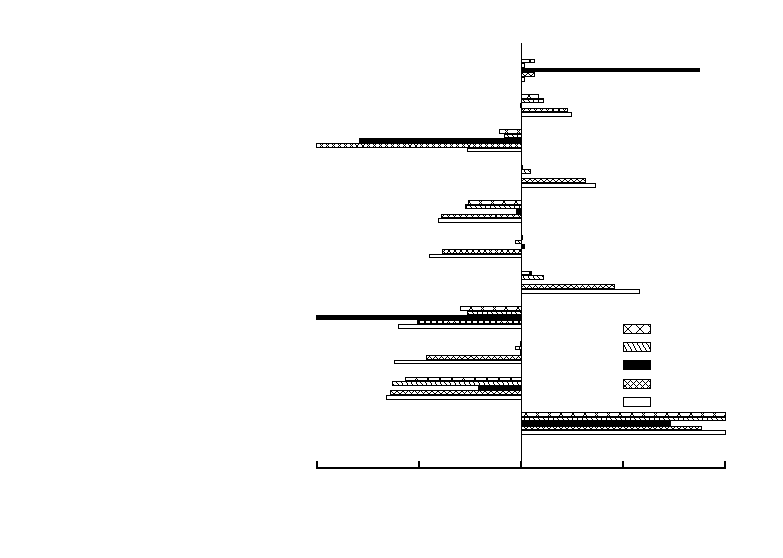
\includegraphics{CEMA_800}}%
    \gplfronttext
  \end{picture}%
\endgroup

  % GNUPLOT: LaTeX picture with Postscript
\begingroup
  \makeatletter
  \providecommand\color[2][]{%
    \GenericError{(gnuplot) \space\space\space\@spaces}{%
      Package color not loaded in conjunction with
      terminal option `colourtext'%
    }{See the gnuplot documentation for explanation.%
    }{Either use 'blacktext' in gnuplot or load the package
      color.sty in LaTeX.}%
    \renewcommand\color[2][]{}%
  }%
  \providecommand\includegraphics[2][]{%
    \GenericError{(gnuplot) \space\space\space\@spaces}{%
      Package graphicx or graphics not loaded%
    }{See the gnuplot documentation for explanation.%
    }{The gnuplot epslatex terminal needs graphicx.sty or graphics.sty.}%
    \renewcommand\includegraphics[2][]{}%
  }%
  \providecommand\rotatebox[2]{#2}%
  \@ifundefined{ifGPcolor}{%
    \newif\ifGPcolor
    \GPcolortrue
  }{}%
  \@ifundefined{ifGPblacktext}{%
    \newif\ifGPblacktext
    \GPblacktexttrue
  }{}%
  % define a \g@addto@macro without @ in the name:
  \let\gplgaddtomacro\g@addto@macro
  % define empty templates for all commands taking text:
  \gdef\gplbacktext{}%
  \gdef\gplfronttext{}%
  \makeatother
  \ifGPblacktext
    % no textcolor at all
    \def\colorrgb#1{}%
    \def\colorgray#1{}%
  \else
    % gray or color?
    \ifGPcolor
      \def\colorrgb#1{\color[rgb]{#1}}%
      \def\colorgray#1{\color[gray]{#1}}%
      \expandafter\def\csname LTw\endcsname{\color{white}}%
      \expandafter\def\csname LTb\endcsname{\color{black}}%
      \expandafter\def\csname LTa\endcsname{\color{black}}%
      \expandafter\def\csname LT0\endcsname{\color[rgb]{1,0,0}}%
      \expandafter\def\csname LT1\endcsname{\color[rgb]{0,1,0}}%
      \expandafter\def\csname LT2\endcsname{\color[rgb]{0,0,1}}%
      \expandafter\def\csname LT3\endcsname{\color[rgb]{1,0,1}}%
      \expandafter\def\csname LT4\endcsname{\color[rgb]{0,1,1}}%
      \expandafter\def\csname LT5\endcsname{\color[rgb]{1,1,0}}%
      \expandafter\def\csname LT6\endcsname{\color[rgb]{0,0,0}}%
      \expandafter\def\csname LT7\endcsname{\color[rgb]{1,0.3,0}}%
      \expandafter\def\csname LT8\endcsname{\color[rgb]{0.5,0.5,0.5}}%
    \else
      % gray
      \def\colorrgb#1{\color{black}}%
      \def\colorgray#1{\color[gray]{#1}}%
      \expandafter\def\csname LTw\endcsname{\color{white}}%
      \expandafter\def\csname LTb\endcsname{\color{black}}%
      \expandafter\def\csname LTa\endcsname{\color{black}}%
      \expandafter\def\csname LT0\endcsname{\color{black}}%
      \expandafter\def\csname LT1\endcsname{\color{black}}%
      \expandafter\def\csname LT2\endcsname{\color{black}}%
      \expandafter\def\csname LT3\endcsname{\color{black}}%
      \expandafter\def\csname LT4\endcsname{\color{black}}%
      \expandafter\def\csname LT5\endcsname{\color{black}}%
      \expandafter\def\csname LT6\endcsname{\color{black}}%
      \expandafter\def\csname LT7\endcsname{\color{black}}%
      \expandafter\def\csname LT8\endcsname{\color{black}}%
    \fi
  \fi
  \setlength{\unitlength}{0.0500bp}%
  \begin{picture}(7200.00,5040.00)%
    \gplgaddtomacro\gplbacktext{%
      \csname LTb\endcsname%
      \put(2748,1043){\makebox(0,0)[r]{\strut{}CH$_3$OCH$_2$$\Longleftrightarrow$CH$_2$O+CH$_3$}}%
      \put(2748,1383){\makebox(0,0)[r]{\strut{}CH$_3$OCH$_2$O$_2$$\Longleftrightarrow$CH$_2$OCH$_2$O$_2$H}}%
      \put(2748,1722){\makebox(0,0)[r]{\strut{}CH$_3$OCH$_3$+CH$_3$$\Longleftrightarrow$CH$_3$OCH$_2$+CH$_4$}}%
      \put(2748,2061){\makebox(0,0)[r]{\strut{}CH$_3$OCH$_3$+HO$_2$$\Longleftrightarrow$CH$_3$OCH$_2$+H$_2$O$_2$}}%
      \put(2748,2400){\makebox(0,0)[r]{\strut{}CH$_3$+CH$_3$+M$\Longleftrightarrow$C$_2$H$_6$+M}}%
      \put(2748,2740){\makebox(0,0)[r]{\strut{}CH$_3$+HO$_2$$\Longleftrightarrow$CH$_3$O+OH}}%
      \put(2748,3079){\makebox(0,0)[r]{\strut{}CH$_3$+HO$_2$$\Longleftrightarrow$CH$_4$+O$_2$}}%
      \put(2748,3418){\makebox(0,0)[r]{\strut{}CH$_2$OCH$_2$O$_2$H$\Longleftrightarrow$OH+CH$_2$O+CH$_2$O}}%
      \put(2748,3757){\makebox(0,0)[r]{\strut{}H$_2$O$_2$+M$\Longleftrightarrow$OH+OH+M}}%
      \put(2748,4097){\makebox(0,0)[r]{\strut{}H+O$_2$+M$\Longleftrightarrow$HO$_2$+M}}%
      \put(2748,4436){\makebox(0,0)[r]{\strut{}H+O$_2$$\Longleftrightarrow$O+OH}}%
      \put(2880,484){\makebox(0,0){\strut{}-1}}%
      \put(3861,484){\makebox(0,0){\strut{}-0.5}}%
      \put(4842,484){\makebox(0,0){\strut{} 0}}%
      \put(5822,484){\makebox(0,0){\strut{} 0.5}}%
      \put(6803,484){\makebox(0,0){\strut{} 1}}%
      \csname LTb\endcsname%
      \put(4841,154){\makebox(0,0){\strut{}Normalized Participation Index}}%
      \put(3076,1349){\makebox(0,0)[l]{\strut{}Point A}}%
      \put(3076,1518){\makebox(0,0)[l]{\strut{}Point B}}%
      \put(3076,1688){\makebox(0,0)[l]{\strut{}Point C}}%
      \put(3076,1857){\makebox(0,0)[l]{\strut{}Point D}}%
      \put(3076,2027){\makebox(0,0)[l]{\strut{}Point E}}%
      \put(3076,2231){\makebox(0,0)[l]{\strut{}$1100$ K}}%
    }%
    \gplgaddtomacro\gplfronttext{%
      \csname LTb\endcsname%
      \put(3532,1337){\makebox(0,0)[r]{\strut{} }}%
      \csname LTb\endcsname%
      \put(3532,1513){\makebox(0,0)[r]{\strut{} }}%
      \csname LTb\endcsname%
      \put(3532,1689){\makebox(0,0)[r]{\strut{} }}%
      \csname LTb\endcsname%
      \put(3532,1865){\makebox(0,0)[r]{\strut{} }}%
      \csname LTb\endcsname%
      \put(3532,2041){\makebox(0,0)[r]{\strut{} }}%
    }%
    \gplbacktext
    \put(0,0){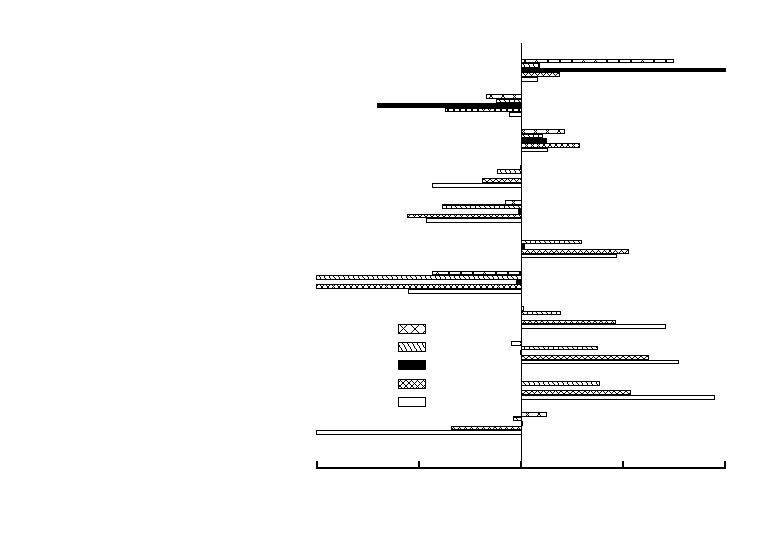
\includegraphics{CEMA_1100}}%
    \gplfronttext
  \end{picture}%
\endgroup

  \normalsize
  \caption{Normalized participation index at $800$ K and $1100$ K.  Sampled locations are indicated in Fig.~\ref{fig:dynamics-HRR_T}.}
  \label{fig:CEMA_T}
\end{figure}

The results are summarized in Fig.~\ref{fig:CEMA_T}, where three representative locations along the $Z_{\rm st}$ iso-contour approaching the flame front and two locations ahead of and at the reaction front at $Z = 0.2$ were sampled.  For the three lower coflow temperature cases, similar chemical patterns were found.  Upstream of the flame front, the chemical explosive mode is positive, indicating that the mixtures have the potential to explode; downstream of the flame front, the chemical explosive mode becomes negative, meaning that the mixtures are composed of burned products.  Following the $Z_{\rm st}$ iso-contour, the hydrogen peroxide chain branching reaction (H$_2$O$_2$ + M $\Longleftrightarrow$ OH + OH + M) is the reaction that has the largest contribution to the explosive mode, showing the dominant role of autoignition chain branching~\cite{westbrook00}.  The characteristic DME low-temperature chemistry is also important upstream of the flame, where methoxymethylperoxy radical formation (CH$_3$OCH$_2$ + O$_2$ $\Longleftrightarrow$ CH$_3$OCH$_2$O$_2$) and isomerization (CH$_3$OCH$_2$O$_2$ $\Longleftrightarrow$ CH$_2$OCH$_2$O$_2$H) promote the explosion, while the $\beta$-scission reaction (CH$_2$OCH$_2$O$_2$H $\Longleftrightarrow$ OH + CH$_2$O + CH$_2$O) retards the explosion.  Approaching the flame front, the H radical recombination reaction (H + O$_2$ + M $\Longleftrightarrow$ HO$_2$ + M) becomes important for the $700-900$ K cases, due to the fact that the H radicals generated at the reaction zone diffuse upstream and undergo three-body recombination reactions under the high pressure, low temperature condition.  Further downstream where the heat release rate peaks, the hydrogen branching reaction (H + O$_2$ $\Longleftrightarrow$ O + OH) becomes the most important chain branching reaction as it is activated at high temperatures~\cite{westbrook00}.

CEMA conducted along the $Z = 0.2$ iso-contour, which crosses the rich heat release front in the $800$ and $900$ K cases, shows different chemical mode evolution.  The H$_2$O$_2$ chain branching reaction is always the dominant reaction that promotes the explosive mode, while the H radical recombination reaction and the H branching reaction are less important ahead of the rich heat release front and at the front.  

On the contrary, although low-temperature chemistry is still important for the $1100$ K case upstream of the reaction zone and the hydrogen chain branching reaction promotes explosion in the reaction zone, the hydrogen peroxide chain branching reaction is not very important for all the sampled locations.  Since the hydrogen peroxide reaction is the crucial chain branching reaction for the autoignition process, it is concluded that the $1100$ K case is less affected by autoignition chemistry than the lower boundary temperature cases.  

\subsubsection{Lagrangian Flamelet Analysis} \label{sec:LFA}

The above species profile analysis and CEMA results have demonstrated that autoignition chemistry is crucial to the complex flame structure in the $700$ to $900$ K cases.  However, the role that autoignition plays in the stabilization still needs further investigation.  To elucidate the role of autoignition for the current flow configuration, a direct comparison with the homogeneous counterpart for a Lagrangian flow particle is insufficient, for no transport process is considered in homogeneous autoignition.  In the current two-dimensional configuration, however, transport processes are present in two directions: parallel and normal to the mixture fraction gradient.  These transport processes might be important: first, the temperature and species stratification parallel to the mixture fraction gradient can significantly modify the ignition characteristics, especially for fuels with NTC chemistry, as shown in Chapter~\ref{ch:NTC}.  Second, flame propagation normal to the mixture fraction gradient can also influence the autoignition front through thermal and radical back diffusion.

To demonstrate the dominant transport direction as well as the stabilization mechanism, one-dimensional unsteady flamelet analysis was conducted to account for unsteadiness (convection), chemical reactions, and diffusion parallel to the mixture fraction gradient, while neglecting the transport process in the normal direction.  As a consequence, the unsteady flamelet is able to capture inhomogeneous autoignition, with diffusion allowed only in one direction.  Following the mixture fraction iso-contour, the spatial information from the two-dimensional computation could be interpreted as the time history of the corresponding mixture in the Lagrangian frame.  If the one-dimensional unsteady flamelet predicts this time history, only the transport processes parallel to the mixture fraction gradient are important, and, therefore, the thermal structure is stabilized by inhomogeneous autoignition.  Conversely, if the unsteady flamelet solutions do not agree with the two-dimensional computations, the transport processes along the mixture fraction iso-contour are not negligible compared to the gradient direction.  Therefore, premixed flame propagation is the dominant stabilization mechanism, or, at least, stabilization is strongly affected by flame back diffusion.

The unsteady flamelet model developed by Pitsch \emph{et al.}~\cite{pitsch98a}, referred to as Lagrangian Flamelet Analysis (LFA), was adopted.  Due to the mixing processes, the scalar dissipation rate $\chi$, which can influence the flamelet solution significantly, decreases in the streamwise direction.  Therefore, this dissipation rate variation must be considered when computing a flamelet as it evolves downstream.

The unsteady flamelet was computed with FlameMaster~\cite{flamemaster}, and the dissipation rate was specified as a function of the flamelet time.  The flamelet time was computed from the two-dimensional computational results, along the stoichiometric mixture fraction $Z_{\rm st}$ iso-contour: 
 \begin{equation} \label{eq:t}
t = \int ^{x}_{0} \frac{1}{(u + u_Z)(x')|(Z=Z_{\rm st})} dx'.
\end{equation}
This formulation is otherwise the same as that of Pitsch \emph {et al.}~\cite{pitsch98a}, except that, in addition to the axial component of fluid convection velocity $u$, the axial component of the mixture fraction iso-contour propagation speed relative to the fluid convection $u_Z$ is also taken into account.  The expression for the constant property scalar iso-surface velocity relative to the local fluid motion was derived by Pope~\cite{pope88}, and the current work adopts the formulation derived by Lignell \emph {et al.}~\cite{lignell07} for variable properties:
\begin{equation}
\mathbf{u_Z} = -\frac{\nabla \cdot (\rho D_Z \nabla Z) }{\rho |\nabla Z|} \mathbf{n},
\end{equation}  
where $D_Z$ is the mixture fraction diffusivity, which is defined in Sec.~\ref{sec:dynamics-computation}, and $\rho$ the density.  The normal vector \textbf{n}, defined as
\begin{equation}
\mathbf{n} = \frac{\nabla Z}{|\nabla Z|},
\end{equation}
indicates the direction of this diffusion induced relative velocity.
The dissipation rate along the $Z_{\rm st} = 0.1005$ iso-contour obtained from the two-dimensional computation was then correlated with this flamelet time and provided as the input for the LFA calculation.  The dissipation rates at other mixture fractions were computed assuming the following form~\cite{petersbook}:
\begin{equation} \label{eq:Zref}
\chi{(Z)} = \chi{(Z_{\rm st})} \frac{\exp{(-2[{\rm erfc}^{-1}(2Z)]^2)}}{\exp{(-2[{\rm erfc}^{-1}(2Z_{\rm st})]^2)}} = \chi{(Z_{\rm st})} f(Z;Z_{\rm st}).
\end{equation}

To validate this formulation in the current configuration, the dissipation rates along different mixture fraction iso-contours were sampled from the two-dimensional computations, normalized using Eq.~\ref{eq:Zref}, and compared with the sampling along the $Z_{\rm st}$ iso-contour.  As shown in Fig.~\ref{fig:Zref}, the normalized dissipation rates at different mixture fractions all collapse to the value at $Z_{\rm st}$.  Therefore, only the dissipation rate samplings along the $Z_{\rm st}$ iso-contour were needed to perform the unsteady flamelet calculation.

\begin{figure}
  \centering
  \scriptsize
  % GNUPLOT: LaTeX picture with Postscript
\begingroup
  \makeatletter
  \providecommand\color[2][]{%
    \GenericError{(gnuplot) \space\space\space\@spaces}{%
      Package color not loaded in conjunction with
      terminal option `colourtext'%
    }{See the gnuplot documentation for explanation.%
    }{Either use 'blacktext' in gnuplot or load the package
      color.sty in LaTeX.}%
    \renewcommand\color[2][]{}%
  }%
  \providecommand\includegraphics[2][]{%
    \GenericError{(gnuplot) \space\space\space\@spaces}{%
      Package graphicx or graphics not loaded%
    }{See the gnuplot documentation for explanation.%
    }{The gnuplot epslatex terminal needs graphicx.sty or graphics.sty.}%
    \renewcommand\includegraphics[2][]{}%
  }%
  \providecommand\rotatebox[2]{#2}%
  \@ifundefined{ifGPcolor}{%
    \newif\ifGPcolor
    \GPcolortrue
  }{}%
  \@ifundefined{ifGPblacktext}{%
    \newif\ifGPblacktext
    \GPblacktexttrue
  }{}%
  % define a \g@addto@macro without @ in the name:
  \let\gplgaddtomacro\g@addto@macro
  % define empty templates for all commands taking text:
  \gdef\gplbacktext{}%
  \gdef\gplfronttext{}%
  \makeatother
  \ifGPblacktext
    % no textcolor at all
    \def\colorrgb#1{}%
    \def\colorgray#1{}%
  \else
    % gray or color?
    \ifGPcolor
      \def\colorrgb#1{\color[rgb]{#1}}%
      \def\colorgray#1{\color[gray]{#1}}%
      \expandafter\def\csname LTw\endcsname{\color{white}}%
      \expandafter\def\csname LTb\endcsname{\color{black}}%
      \expandafter\def\csname LTa\endcsname{\color{black}}%
      \expandafter\def\csname LT0\endcsname{\color[rgb]{1,0,0}}%
      \expandafter\def\csname LT1\endcsname{\color[rgb]{0,1,0}}%
      \expandafter\def\csname LT2\endcsname{\color[rgb]{0,0,1}}%
      \expandafter\def\csname LT3\endcsname{\color[rgb]{1,0,1}}%
      \expandafter\def\csname LT4\endcsname{\color[rgb]{0,1,1}}%
      \expandafter\def\csname LT5\endcsname{\color[rgb]{1,1,0}}%
      \expandafter\def\csname LT6\endcsname{\color[rgb]{0,0,0}}%
      \expandafter\def\csname LT7\endcsname{\color[rgb]{1,0.3,0}}%
      \expandafter\def\csname LT8\endcsname{\color[rgb]{0.5,0.5,0.5}}%
    \else
      % gray
      \def\colorrgb#1{\color{black}}%
      \def\colorgray#1{\color[gray]{#1}}%
      \expandafter\def\csname LTw\endcsname{\color{white}}%
      \expandafter\def\csname LTb\endcsname{\color{black}}%
      \expandafter\def\csname LTa\endcsname{\color{black}}%
      \expandafter\def\csname LT0\endcsname{\color{black}}%
      \expandafter\def\csname LT1\endcsname{\color{black}}%
      \expandafter\def\csname LT2\endcsname{\color{black}}%
      \expandafter\def\csname LT3\endcsname{\color{black}}%
      \expandafter\def\csname LT4\endcsname{\color{black}}%
      \expandafter\def\csname LT5\endcsname{\color{black}}%
      \expandafter\def\csname LT6\endcsname{\color{black}}%
      \expandafter\def\csname LT7\endcsname{\color{black}}%
      \expandafter\def\csname LT8\endcsname{\color{black}}%
    \fi
  \fi
  \setlength{\unitlength}{0.0500bp}%
  \begin{picture}(7200.00,5040.00)%
    \gplgaddtomacro\gplbacktext{%
      \csname LTb\endcsname%
      \put(946,704){\makebox(0,0)[r]{\strut{} 0}}%
      \put(946,1383){\makebox(0,0)[r]{\strut{} 50}}%
      \put(946,2061){\makebox(0,0)[r]{\strut{} 100}}%
      \put(946,2740){\makebox(0,0)[r]{\strut{} 150}}%
      \put(946,3418){\makebox(0,0)[r]{\strut{} 200}}%
      \put(946,4097){\makebox(0,0)[r]{\strut{} 250}}%
      \put(946,4775){\makebox(0,0)[r]{\strut{} 300}}%
      \put(1078,484){\makebox(0,0){\strut{} 0}}%
      \put(1841,484){\makebox(0,0){\strut{} 0.2}}%
      \put(2605,484){\makebox(0,0){\strut{} 0.4}}%
      \put(3368,484){\makebox(0,0){\strut{} 0.6}}%
      \put(4131,484){\makebox(0,0){\strut{} 0.8}}%
      \put(4895,484){\makebox(0,0){\strut{} 1}}%
      \put(5658,484){\makebox(0,0){\strut{} 1.2}}%
      \put(6421,484){\makebox(0,0){\strut{} 1.4}}%
      \put(176,2739){\rotatebox{-270}{\makebox(0,0){\strut{}\vspace{-28pt}$\frac{\chi(Z)}{f(Z,Z_{\rm st})}$ [1/s]}}}%
      \put(3940,154){\makebox(0,0){\strut{}Time [ms]}}%
    }%
    \gplgaddtomacro\gplfronttext{%
      \csname LTb\endcsname%
      \put(5816,4602){\makebox(0,0)[r]{\strut{}$Z = Z_{\rm st}$}}%
      \csname LTb\endcsname%
      \put(5816,4382){\makebox(0,0)[r]{\strut{}$Z = 0.2$}}%
      \csname LTb\endcsname%
      \put(5816,4162){\makebox(0,0)[r]{\strut{}$Z = 0.4$}}%
      \csname LTb\endcsname%
      \put(5816,3942){\makebox(0,0)[r]{\strut{}$Z = 0.6$}}%
    }%
    \gplbacktext
    \put(0,0){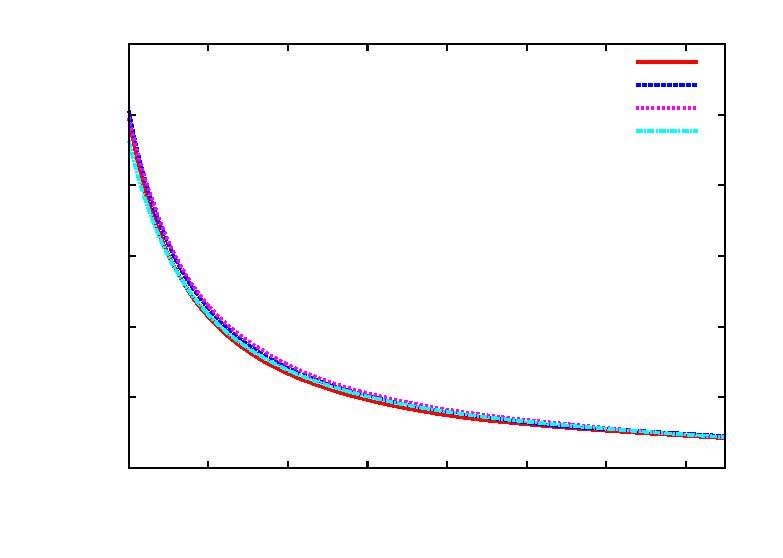
\includegraphics{Zref}}%
    \gplfronttext
  \end{picture}%
\endgroup

  \normalsize
  \caption{$\frac{\chi(Z)}{f(Z;Z_{\rm st})}$, using Eq.~\ref{eq:Zref}, from the two-dimensional calculations at $800$ K.}
  \label{fig:Zref}
\end{figure}

To account for the differential diffusion, species Lewis numbers for LFA  were specified the same as in the two-dimensional computations.  The governing equations for species and temperature follow Eq. $24$ and $25$ in Pitsch and Peters~\cite{pitsch98b}.

The time history of the dissipation rate $\chi_{\rm st}$ was specified in LFA according to the two-dimensional computation.  To avoid the ill-defined Lagrangian time in the recirculation zone, time zero was defined at a downstream location ten times the thickness of the wall.  Accordingly, the species and temperature profiles along the radial cut at this location were specified as the initial conditions for the flamelet.  Based on these initial conditions and $\chi_{\rm st}$ time history profiles, the unsteady flamelets were calculated and compared with the two-dimensional computational results for $Z_{\rm st}$, $Z = 0.2$, and $Z = 0.3$.

\begin{figure}
  \centering
  \scriptsize
  \resizebox{1.15\textwidth}{!}{% GNUPLOT: LaTeX picture with Postscript
\begingroup
  \makeatletter
  \providecommand\color[2][]{%
    \GenericError{(gnuplot) \space\space\space\@spaces}{%
      Package color not loaded in conjunction with
      terminal option `colourtext'%
    }{See the gnuplot documentation for explanation.%
    }{Either use 'blacktext' in gnuplot or load the package
      color.sty in LaTeX.}%
    \renewcommand\color[2][]{}%
  }%
  \providecommand\includegraphics[2][]{%
    \GenericError{(gnuplot) \space\space\space\@spaces}{%
      Package graphicx or graphics not loaded%
    }{See the gnuplot documentation for explanation.%
    }{The gnuplot epslatex terminal needs graphicx.sty or graphics.sty.}%
    \renewcommand\includegraphics[2][]{}%
  }%
  \providecommand\rotatebox[2]{#2}%
  \@ifundefined{ifGPcolor}{%
    \newif\ifGPcolor
    \GPcolortrue
  }{}%
  \@ifundefined{ifGPblacktext}{%
    \newif\ifGPblacktext
    \GPblacktexttrue
  }{}%
  % define a \g@addto@macro without @ in the name:
  \let\gplgaddtomacro\g@addto@macro
  % define empty templates for all commands taking text:
  \gdef\gplbacktext{}%
  \gdef\gplfronttext{}%
  \makeatother
  \ifGPblacktext
    % no textcolor at all
    \def\colorrgb#1{}%
    \def\colorgray#1{}%
  \else
    % gray or color?
    \ifGPcolor
      \def\colorrgb#1{\color[rgb]{#1}}%
      \def\colorgray#1{\color[gray]{#1}}%
      \expandafter\def\csname LTw\endcsname{\color{white}}%
      \expandafter\def\csname LTb\endcsname{\color{black}}%
      \expandafter\def\csname LTa\endcsname{\color{black}}%
      \expandafter\def\csname LT0\endcsname{\color[rgb]{1,0,0}}%
      \expandafter\def\csname LT1\endcsname{\color[rgb]{0,1,0}}%
      \expandafter\def\csname LT2\endcsname{\color[rgb]{0,0,1}}%
      \expandafter\def\csname LT3\endcsname{\color[rgb]{1,0,1}}%
      \expandafter\def\csname LT4\endcsname{\color[rgb]{0,1,1}}%
      \expandafter\def\csname LT5\endcsname{\color[rgb]{1,1,0}}%
      \expandafter\def\csname LT6\endcsname{\color[rgb]{0,0,0}}%
      \expandafter\def\csname LT7\endcsname{\color[rgb]{1,0.3,0}}%
      \expandafter\def\csname LT8\endcsname{\color[rgb]{0.5,0.5,0.5}}%
    \else
      % gray
      \def\colorrgb#1{\color{black}}%
      \def\colorgray#1{\color[gray]{#1}}%
      \expandafter\def\csname LTw\endcsname{\color{white}}%
      \expandafter\def\csname LTb\endcsname{\color{black}}%
      \expandafter\def\csname LTa\endcsname{\color{black}}%
      \expandafter\def\csname LT0\endcsname{\color{black}}%
      \expandafter\def\csname LT1\endcsname{\color{black}}%
      \expandafter\def\csname LT2\endcsname{\color{black}}%
      \expandafter\def\csname LT3\endcsname{\color{black}}%
      \expandafter\def\csname LT4\endcsname{\color{black}}%
      \expandafter\def\csname LT5\endcsname{\color{black}}%
      \expandafter\def\csname LT6\endcsname{\color{black}}%
      \expandafter\def\csname LT7\endcsname{\color{black}}%
      \expandafter\def\csname LT8\endcsname{\color{black}}%
    \fi
  \fi
  \setlength{\unitlength}{0.0500bp}%
  \begin{picture}(11520.00,6048.00)%
    \gplgaddtomacro\gplbacktext{%
      \csname LTb\endcsname%
      \put(7990,4756){\makebox(0,0)[r]{\strut{} 800}}%
      \put(7990,4961){\makebox(0,0)[r]{\strut{} 1200}}%
      \put(7990,5167){\makebox(0,0)[r]{\strut{} 1600}}%
      \put(7990,5372){\makebox(0,0)[r]{\strut{} 2000}}%
      \put(7990,5578){\makebox(0,0)[r]{\strut{} 2400}}%
      \put(7990,5783){\makebox(0,0)[r]{\strut{} 2800}}%
      \put(8122,4536){\makebox(0,0){\strut{} 0}}%
      \put(8440,4536){\makebox(0,0){\strut{} 0.25}}%
      \put(8759,4536){\makebox(0,0){\strut{} 0.5}}%
      \put(9077,4536){\makebox(0,0){\strut{} 0.75}}%
      \put(9395,4536){\makebox(0,0){\strut{} 1}}%
      \put(7088,5269){\rotatebox{-270}{\makebox(0,0){\strut{}\vspace{-48pt}$T$ [K]}}}%
      \put(8758,4206){\makebox(0,0){\strut{}\vspace{12pt}Time [ms]}}%
      \put(1728,6047){\makebox(0,0)[l]{\strut{}$700$ K}}%
      \put(4032,6047){\makebox(0,0)[l]{\strut{}$800$ K}}%
      \put(6335,6047){\makebox(0,0)[l]{\strut{}$900$ K}}%
      \put(8639,6047){\makebox(0,0)[l]{\strut{}$1100$ K}}%
      \put(-229,1209){\makebox(0,0)[l]{\strut{}$Z = 0.3$}}%
      \put(-229,3205){\makebox(0,0)[l]{\strut{}$Z = 0.2$}}%
      \put(-229,5261){\makebox(0,0)[l]{\strut{}$Z = Z_{\rm st}$}}%
    }%
    \gplgaddtomacro\gplfronttext{%
    }%
    \gplgaddtomacro\gplbacktext{%
      \csname LTb\endcsname%
      \put(7990,2941){\makebox(0,0)[r]{\strut{} 800}}%
      \put(7990,3147){\makebox(0,0)[r]{\strut{} 1200}}%
      \put(7990,3352){\makebox(0,0)[r]{\strut{} 1600}}%
      \put(7990,3558){\makebox(0,0)[r]{\strut{} 2000}}%
      \put(7990,3763){\makebox(0,0)[r]{\strut{} 2400}}%
      \put(7990,3969){\makebox(0,0)[r]{\strut{} 2800}}%
      \put(8122,2721){\makebox(0,0){\strut{} 0}}%
      \put(8440,2721){\makebox(0,0){\strut{} 0.25}}%
      \put(8759,2721){\makebox(0,0){\strut{} 0.5}}%
      \put(9077,2721){\makebox(0,0){\strut{} 0.75}}%
      \put(9395,2721){\makebox(0,0){\strut{} 1}}%
      \put(7088,3455){\rotatebox{-270}{\makebox(0,0){\strut{}\vspace{-48pt}$T$ [K]}}}%
      \put(8758,2391){\makebox(0,0){\strut{}\vspace{12pt}Time [ms]}}%
    }%
    \gplgaddtomacro\gplfronttext{%
    }%
    \gplgaddtomacro\gplbacktext{%
      \csname LTb\endcsname%
      \put(7990,1187){\makebox(0,0)[r]{\strut{} 400}}%
      \put(7990,1393){\makebox(0,0)[r]{\strut{} 800}}%
      \put(7990,1598){\makebox(0,0)[r]{\strut{} 1200}}%
      \put(7990,1804){\makebox(0,0)[r]{\strut{} 1600}}%
      \put(7990,2009){\makebox(0,0)[r]{\strut{} 2000}}%
      \put(7990,2215){\makebox(0,0)[r]{\strut{} 2400}}%
      \put(8122,967){\makebox(0,0){\strut{} 0}}%
      \put(8440,967){\makebox(0,0){\strut{} 0.25}}%
      \put(8759,967){\makebox(0,0){\strut{} 0.5}}%
      \put(9077,967){\makebox(0,0){\strut{} 0.75}}%
      \put(9395,967){\makebox(0,0){\strut{} 1}}%
      \put(7088,1701){\rotatebox{-270}{\makebox(0,0){\strut{}\vspace{-48pt}$T$ [K]}}}%
      \put(8758,637){\makebox(0,0){\strut{}\vspace{12pt}Time [ms]}}%
    }%
    \gplgaddtomacro\gplfronttext{%
    }%
    \gplgaddtomacro\gplbacktext{%
      \csname LTb\endcsname%
      \put(5686,4756){\makebox(0,0)[r]{\strut{} 600}}%
      \put(5686,4961){\makebox(0,0)[r]{\strut{} 1000}}%
      \put(5686,5167){\makebox(0,0)[r]{\strut{} 1400}}%
      \put(5686,5372){\makebox(0,0)[r]{\strut{} 1800}}%
      \put(5686,5578){\makebox(0,0)[r]{\strut{} 2200}}%
      \put(5686,5783){\makebox(0,0)[r]{\strut{} 2600}}%
      \put(5818,4536){\makebox(0,0){\strut{} 0}}%
      \put(6136,4536){\makebox(0,0){\strut{} 0.3}}%
      \put(6455,4536){\makebox(0,0){\strut{} 0.6}}%
      \put(6773,4536){\makebox(0,0){\strut{} 0.9}}%
      \put(7091,4536){\makebox(0,0){\strut{} 1.2}}%
      \put(4784,5269){\rotatebox{-270}{\makebox(0,0){\strut{}\vspace{-48pt}$T$ [K]}}}%
      \put(6454,4206){\makebox(0,0){\strut{}\vspace{12pt}Time [ms]}}%
    }%
    \gplgaddtomacro\gplfronttext{%
    }%
    \gplgaddtomacro\gplbacktext{%
      \csname LTb\endcsname%
      \put(5686,2941){\makebox(0,0)[r]{\strut{} 600}}%
      \put(5686,3147){\makebox(0,0)[r]{\strut{} 1000}}%
      \put(5686,3352){\makebox(0,0)[r]{\strut{} 1400}}%
      \put(5686,3558){\makebox(0,0)[r]{\strut{} 1800}}%
      \put(5686,3763){\makebox(0,0)[r]{\strut{} 2200}}%
      \put(5686,3969){\makebox(0,0)[r]{\strut{} 2600}}%
      \put(5818,2721){\makebox(0,0){\strut{} 0}}%
      \put(6136,2721){\makebox(0,0){\strut{} 0.3}}%
      \put(6455,2721){\makebox(0,0){\strut{} 0.6}}%
      \put(6773,2721){\makebox(0,0){\strut{} 0.9}}%
      \put(7091,2721){\makebox(0,0){\strut{} 1.2}}%
      \put(4784,3455){\rotatebox{-270}{\makebox(0,0){\strut{}\vspace{-48pt}$T$ [K]}}}%
      \put(6454,2391){\makebox(0,0){\strut{}\vspace{12pt}Time [ms]}}%
    }%
    \gplgaddtomacro\gplfronttext{%
    }%
    \gplgaddtomacro\gplbacktext{%
      \csname LTb\endcsname%
      \put(5686,1187){\makebox(0,0)[r]{\strut{} 400}}%
      \put(5686,1393){\makebox(0,0)[r]{\strut{} 800}}%
      \put(5686,1598){\makebox(0,0)[r]{\strut{} 1200}}%
      \put(5686,1804){\makebox(0,0)[r]{\strut{} 1600}}%
      \put(5686,2009){\makebox(0,0)[r]{\strut{} 2000}}%
      \put(5686,2215){\makebox(0,0)[r]{\strut{} 2400}}%
      \put(5818,967){\makebox(0,0){\strut{} 0}}%
      \put(6136,967){\makebox(0,0){\strut{} 0.3}}%
      \put(6455,967){\makebox(0,0){\strut{} 0.6}}%
      \put(6773,967){\makebox(0,0){\strut{} 0.9}}%
      \put(7091,967){\makebox(0,0){\strut{} 1.2}}%
      \put(4784,1701){\rotatebox{-270}{\makebox(0,0){\strut{}\vspace{-48pt}$T$ [K]}}}%
      \put(6454,637){\makebox(0,0){\strut{}\vspace{12pt}Time [ms]}}%
    }%
    \gplgaddtomacro\gplfronttext{%
    }%
    \gplgaddtomacro\gplbacktext{%
      \csname LTb\endcsname%
      \put(3382,4756){\makebox(0,0)[r]{\strut{} 600}}%
      \put(3382,4961){\makebox(0,0)[r]{\strut{} 1000}}%
      \put(3382,5167){\makebox(0,0)[r]{\strut{} 1400}}%
      \put(3382,5372){\makebox(0,0)[r]{\strut{} 1800}}%
      \put(3382,5578){\makebox(0,0)[r]{\strut{} 2200}}%
      \put(3382,5783){\makebox(0,0)[r]{\strut{} 2600}}%
      \put(3514,4536){\makebox(0,0){\strut{} 0}}%
      \put(3832,4536){\makebox(0,0){\strut{} 0.6}}%
      \put(4151,4536){\makebox(0,0){\strut{} 1.2}}%
      \put(4469,4536){\makebox(0,0){\strut{} 1.8}}%
      \put(4787,4536){\makebox(0,0){\strut{} 2.4}}%
      \put(2480,5269){\rotatebox{-270}{\makebox(0,0){\strut{}\vspace{-48pt}$T$ [K]}}}%
      \put(4150,4206){\makebox(0,0){\strut{}\vspace{12pt}Time [ms]}}%
    }%
    \gplgaddtomacro\gplfronttext{%
    }%
    \gplgaddtomacro\gplbacktext{%
      \csname LTb\endcsname%
      \put(3382,2941){\makebox(0,0)[r]{\strut{} 600}}%
      \put(3382,3147){\makebox(0,0)[r]{\strut{} 1000}}%
      \put(3382,3352){\makebox(0,0)[r]{\strut{} 1400}}%
      \put(3382,3558){\makebox(0,0)[r]{\strut{} 1800}}%
      \put(3382,3763){\makebox(0,0)[r]{\strut{} 2200}}%
      \put(3382,3969){\makebox(0,0)[r]{\strut{} 2600}}%
      \put(3514,2721){\makebox(0,0){\strut{} 0}}%
      \put(3832,2721){\makebox(0,0){\strut{} 0.6}}%
      \put(4151,2721){\makebox(0,0){\strut{} 1.2}}%
      \put(4469,2721){\makebox(0,0){\strut{} 1.8}}%
      \put(4787,2721){\makebox(0,0){\strut{} 2.4}}%
      \put(2480,3455){\rotatebox{-270}{\makebox(0,0){\strut{}\vspace{-48pt}$T$ [K]}}}%
      \put(4150,2391){\makebox(0,0){\strut{}\vspace{12pt}Time [ms]}}%
    }%
    \gplgaddtomacro\gplfronttext{%
    }%
    \gplgaddtomacro\gplbacktext{%
      \csname LTb\endcsname%
      \put(3382,1187){\makebox(0,0)[r]{\strut{} 400}}%
      \put(3382,1393){\makebox(0,0)[r]{\strut{} 800}}%
      \put(3382,1598){\makebox(0,0)[r]{\strut{} 1200}}%
      \put(3382,1804){\makebox(0,0)[r]{\strut{} 1600}}%
      \put(3382,2009){\makebox(0,0)[r]{\strut{} 2000}}%
      \put(3382,2215){\makebox(0,0)[r]{\strut{} 2400}}%
      \put(3514,967){\makebox(0,0){\strut{} 0}}%
      \put(3832,967){\makebox(0,0){\strut{} 0.6}}%
      \put(4151,967){\makebox(0,0){\strut{} 1.2}}%
      \put(4469,967){\makebox(0,0){\strut{} 1.8}}%
      \put(4787,967){\makebox(0,0){\strut{} 2.4}}%
      \put(2480,1701){\rotatebox{-270}{\makebox(0,0){\strut{}\vspace{-48pt}$T$ [K]}}}%
      \put(4150,637){\makebox(0,0){\strut{}\vspace{12pt}Time [ms]}}%
    }%
    \gplgaddtomacro\gplfronttext{%
    }%
    \gplgaddtomacro\gplbacktext{%
      \csname LTb\endcsname%
      \put(1078,4756){\makebox(0,0)[r]{\strut{} 400}}%
      \put(1078,4961){\makebox(0,0)[r]{\strut{} 800}}%
      \put(1078,5167){\makebox(0,0)[r]{\strut{} 1200}}%
      \put(1078,5372){\makebox(0,0)[r]{\strut{} 1600}}%
      \put(1078,5578){\makebox(0,0)[r]{\strut{} 2000}}%
      \put(1078,5783){\makebox(0,0)[r]{\strut{} 2400}}%
      \put(1210,4536){\makebox(0,0){\strut{} 0}}%
      \put(1528,4536){\makebox(0,0){\strut{} 2.5}}%
      \put(1847,4536){\makebox(0,0){\strut{} 5}}%
      \put(2165,4536){\makebox(0,0){\strut{} 7.5}}%
      \put(2483,4536){\makebox(0,0){\strut{} 10}}%
      \put(176,5269){\rotatebox{-270}{\makebox(0,0){\strut{}\vspace{-48pt}$T$ [K]}}}%
      \put(1846,4206){\makebox(0,0){\strut{}\vspace{12pt}Time [ms]}}%
    }%
    \gplgaddtomacro\gplfronttext{%
    }%
    \gplgaddtomacro\gplbacktext{%
      \csname LTb\endcsname%
      \put(1078,2941){\makebox(0,0)[r]{\strut{} 400}}%
      \put(1078,3147){\makebox(0,0)[r]{\strut{} 800}}%
      \put(1078,3352){\makebox(0,0)[r]{\strut{} 1200}}%
      \put(1078,3558){\makebox(0,0)[r]{\strut{} 1600}}%
      \put(1078,3763){\makebox(0,0)[r]{\strut{} 2000}}%
      \put(1078,3969){\makebox(0,0)[r]{\strut{} 2400}}%
      \put(1210,2721){\makebox(0,0){\strut{} 0}}%
      \put(1528,2721){\makebox(0,0){\strut{} 2.5}}%
      \put(1847,2721){\makebox(0,0){\strut{} 5}}%
      \put(2165,2721){\makebox(0,0){\strut{} 7.5}}%
      \put(2483,2721){\makebox(0,0){\strut{} 10}}%
      \put(176,3455){\rotatebox{-270}{\makebox(0,0){\strut{}\vspace{-48pt}$T$ [K]}}}%
      \put(1846,2391){\makebox(0,0){\strut{}\vspace{12pt}Time [ms]}}%
    }%
    \gplgaddtomacro\gplfronttext{%
    }%
    \gplgaddtomacro\gplbacktext{%
      \csname LTb\endcsname%
      \put(1078,1187){\makebox(0,0)[r]{\strut{} 200}}%
      \put(1078,1393){\makebox(0,0)[r]{\strut{} 600}}%
      \put(1078,1598){\makebox(0,0)[r]{\strut{} 1000}}%
      \put(1078,1804){\makebox(0,0)[r]{\strut{} 1400}}%
      \put(1078,2009){\makebox(0,0)[r]{\strut{} 1800}}%
      \put(1078,2215){\makebox(0,0)[r]{\strut{} 2200}}%
      \put(1210,967){\makebox(0,0){\strut{} 0}}%
      \put(1528,967){\makebox(0,0){\strut{} 2.5}}%
      \put(1847,967){\makebox(0,0){\strut{} 5}}%
      \put(2165,967){\makebox(0,0){\strut{} 7.5}}%
      \put(2483,967){\makebox(0,0){\strut{} 10}}%
      \put(176,1701){\rotatebox{-270}{\makebox(0,0){\strut{}\vspace{-48pt}$T$ [K]}}}%
      \put(1846,637){\makebox(0,0){\strut{}\vspace{12pt}Time [ms]}}%
      \put(4608,242){\makebox(0,0)[l]{\strut{}2D-CFD}}%
      \put(5760,242){\makebox(0,0)[l]{\strut{}1D-LFA}}%
    }%
    \gplgaddtomacro\gplfronttext{%
      \csname LTb\endcsname%
      \put(4050,253){\makebox(0,0)[r]{\strut{} }}%
      \csname LTb\endcsname%
      \put(5169,253){\makebox(0,0)[r]{\strut{}    }}%
    }%
    \gplbacktext
    \put(0,0){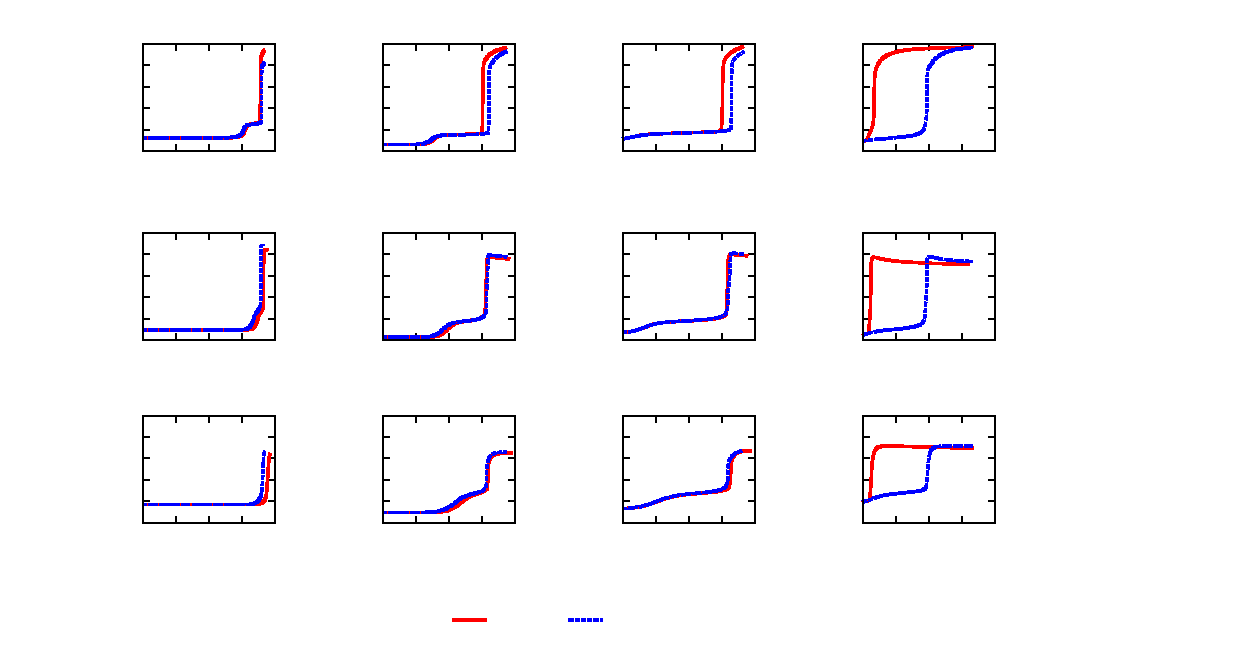
\includegraphics{LFA}}%
    \gplfronttext
  \end{picture}%
\endgroup
}
  \normalsize
  \caption{Comparison between 2D-CFD and 1D-LFA results for the steady cases with the same flow velocities but different boundary temperatures.}
  \label{fig:LFA_T}
\end{figure}

As shown in Fig.~\ref{fig:LFA_T}, two ignition stages can be seen at $Z_{\rm st}$ and $Z = 0.2$ for the $700$ K case, while at $Z = 0.3$ only one ignition dominated by low-temperature chemistry is observed, due to the reduced initial temperature.   At all three mixture fractions examined, the flamelets agree with the two-dimensional computations very well.  For the $800$ K case, both the flamelet and two-dimensional computation experience almost identical time histories, where two-stage ignition occurs at all three mixture fractions.  As the initial temperature further increases, corresponding to the increase in the boundary temperatures in the CFD computation, the two-stage ignition phenomenon is less pronounced.  However, the $900$ K case still shows good agreement between the flamelet profile with the time history of the two-dimensional computation at $Z = 0.2$ and $0.3$, while LFA slightly lags behind the CFD computation at $Z_{\rm st}$ , similar to the $800$ K case.

On the contrary, for the $1100$ K case, the ignition delay time computed with the one-dimensional flamelet assumption is significantly longer than the two-dimensional counterpart, indicating that transport processes along the mixture fraction iso-contours must be important and that autoignition is less important to the stabilization mechanism.

\subsection{Stabilization Mechanism} \label{sec:regime}

With the above analysis based on species profiles, Chemical Explosive Mode Analysis, and Lagrangian Flamelet Analysis, the transition of the stabilization mechanism and the coupling between autoignition chemistry and flame propagation can be clearly identified.  Two fundamental stabilization mechanisms are relevant: the \emph {kinetic} stabilization mechanism, due to the balance between the autoignition delay time and flow residence time, and the \emph {kinematic} stabilization mechanism, due to the balance between the local premixed flame propagation velocity and the local flow velocity.  

In this stratified composition and temperature field, autoignition and flame propagation are coupled through thermal and radical interactions, for the accumulation of the upstream radicals and heat release from autoignition accelerate the flame propagation velocity.  The flame also transfers heat and radicals through back diffusion processes to the upstream, which could also facilitate autoignition.

The stabilization mechanism was determined by comparing the two-dimensional computations with the one-dimensional inhomogeneous autoignition predicted by LFA.  When these two time history profiles agree well, the case is characterized as \emph{kinetically} stabilized.  Specifically, at $700$ K, the one-dimensional LFA agrees very well with the two-dimensional computation at all of the mixture fractions examined.  Therefore, the $700$ K case is characterized as \emph{kinetically} stabilized.  As the boundary temperature increases, the influences from premixed flame propagation become important, as predictions by LFA lag behind the CFD results for some mixture fractions.  At $800$ K, an autoignition front stabilizes the multibrachial structure at rich mixture fractions, due to the shorter ignition delay time resulting from the NTC chemistry, and a modified triple flame structure stabilizes slightly downstream of this front at leaner mixture fractions, as shown in Fig.~\ref{fig:dynamics-HRR_T}.  Further increasing the boundary temperature results in higher flame propagation velocities.  Therefore, the flame front at leaner mixture fraction depends less on radical accumulation ahead of the flame and propagates upstream, and the stabilization is influenced by both inhomogeneous autoignition and premixed flame propagation.  The transition to a \emph {kinematically} stabilized flame structure is achieved for the $1100$ K case, where the local flame propagation velocity balances the incoming flow velocity.  Therefore, the flame structure stabilizes close to the nozzle exit and depends least on radical accumulation from upstream.  Consequently, the one-dimensional LFA predictions departure from the two-dimensional computation significantly.

Based on the understanding obtained from the current study, further extension of the stabilization regime can be made, as shown in Fig.~\ref{fig:regime_T}.  For fixed inlet flow velocity, when the boundary temperature is sufficiently low, the mixture cannot be autoignited, and it is essentially a frozen flow.  Even when an external ignition source is applied, the flame cannot keep up with the excessive high flow velocity, such that the flame blows out.  When the boundary temperature is high enough to activate autoignition, it occurs far downstream, but the flame propagation velocity still cannot keep up with the flow velocity.  As a consequence, a pure \emph {kinetically} stabilized autoignition front can be achieved, which is similar to the $700$ K case.  Conversely, when the boundary temperature is sufficiently high, the flame stabilizes close to the inlet, where the upstream can be treated as frozen, due to reduced residence time, which is similar to the $1100$ K case.  Therefore, a \emph {kinematically} stabilized classical triple flame structure is achieved.  Further increase in the boundary temperature results in an attached flame with the increased flame speed.  Although not included, an attached flame was computed at $1500$ K.  In between the \emph {kinetically} and \emph {kinematically} stabilized regimes, there is a transitional regime governed by both mechanisms, which corresponds to the $800$ and $900$ K cases.  Due to the NTC behavior of the autoignition chemistry, the stabilization point, in terms of mixture fraction space, varies, and the complex multibrachial flame structure appears.  

\begin{figure}[t]
  \centering
  \scriptsize
  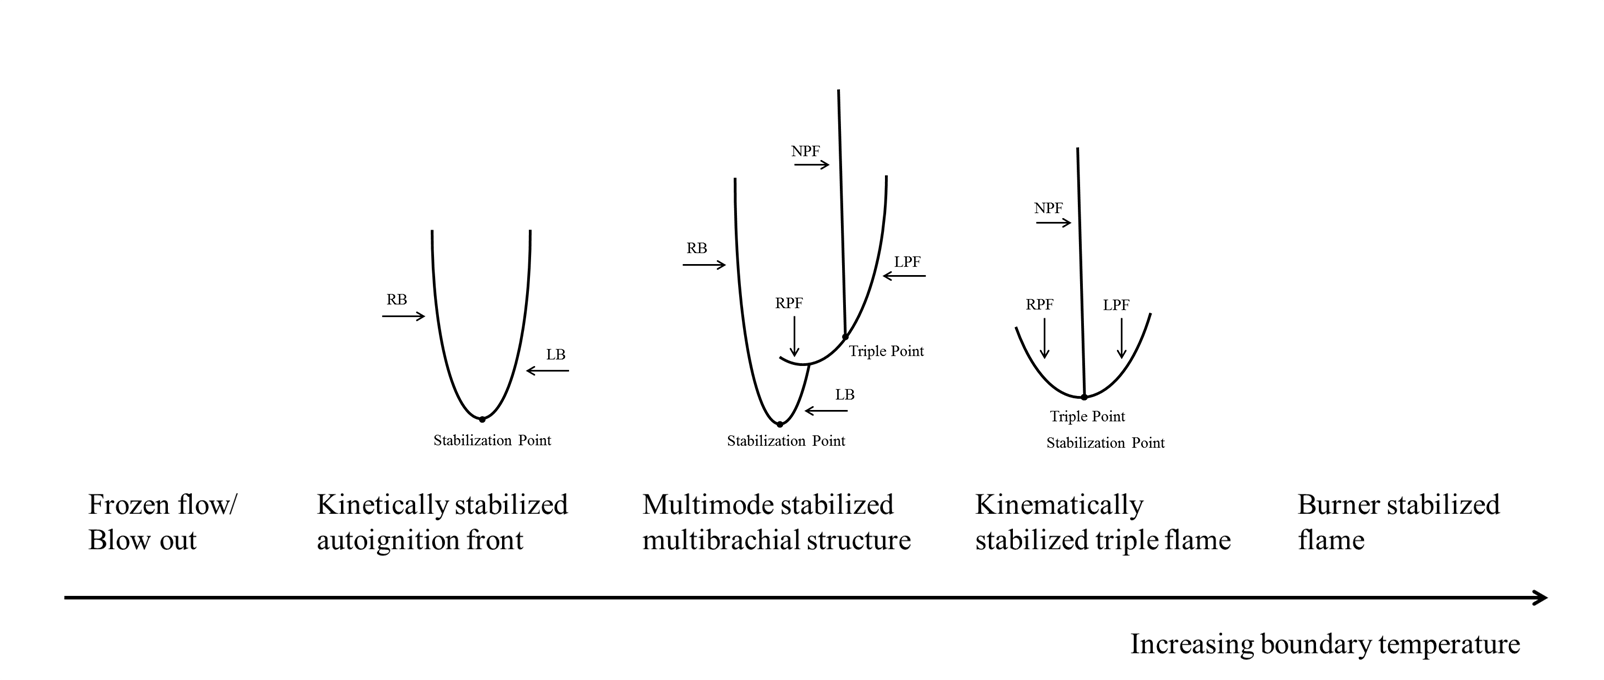
\includegraphics[width=1.0\textwidth]{ch-dynamics/regime.png}
  \normalsize
  \caption{Extended regimes of the stabilization mechanism as the coflow boundary temperature increases.}
  \label{fig:regime_T}
\end{figure}

%--------------------------------------------
\section{Flame Stabilization: Boundary Velocity Effects}\label{sec:dynamics-V}

In this section, the effect of boundary velocity and hence transport on flame stabilization is investigated.  Therefore, in all cases studied in this section, the temperature of the heated air coflow is fixed at $900$ K.  Conversely, the boundary velocities of the DME jet as well as the coflow air are varied ($2.4$, $3.2$, and $8.0$ m/s).  The dimensions of and number of grid points in the computational domain for each computation are summarized in Table~\ref{table:domain_V}.  The $3.2$ m/s case has been presented in Sec.~\ref{sec:dynamics-T}.

\begin{table*}
  \caption{Computational domain and number of grid points for steady cases with the same boundary temperature but different flow velocities.}
  \label{table:domain_V}
  \centering
  \normalsize
  \resizebox{0.6\textwidth}{!}{
  \begin{tabular}{lc*{2}{c}}
    \hline
    Inlet Velocity [m/s]& $2.4$  & $3.2$  & $8.0$   \\
    \hline
    $L_x$ [mm]& $3.5$ & $3.5$ & $15$\\
    %Coflow O.D. [mm]& $3.9$ & $3.9$ & $3.9$\\
    $N_x$ & $1536$ & $1536$  & $3072$\\
    $N_r$ & $176$ & $176$ & $176$\\
    \hline
   \end{tabular}
}
\end{table*}

\subsection{Thermal and Chemical Structure} \label{sec:dynamcis-structure_V}

The heat release rate profiles for the three cases are shown in Fig.~\ref{fig:HRR_V}.  A qualitative determination of the stabilization point is the most upstream point on the largest heat release contour (the leading point), colored by red.  The mixture fraction iso-contours of $Z_{\rm st} = 0.1005$, $Z = 0.2$, and $Z = 0.3$ are delineated in solid black lines, from right to left.

\begin{figure}[t]
  \centering
  \scriptsize
  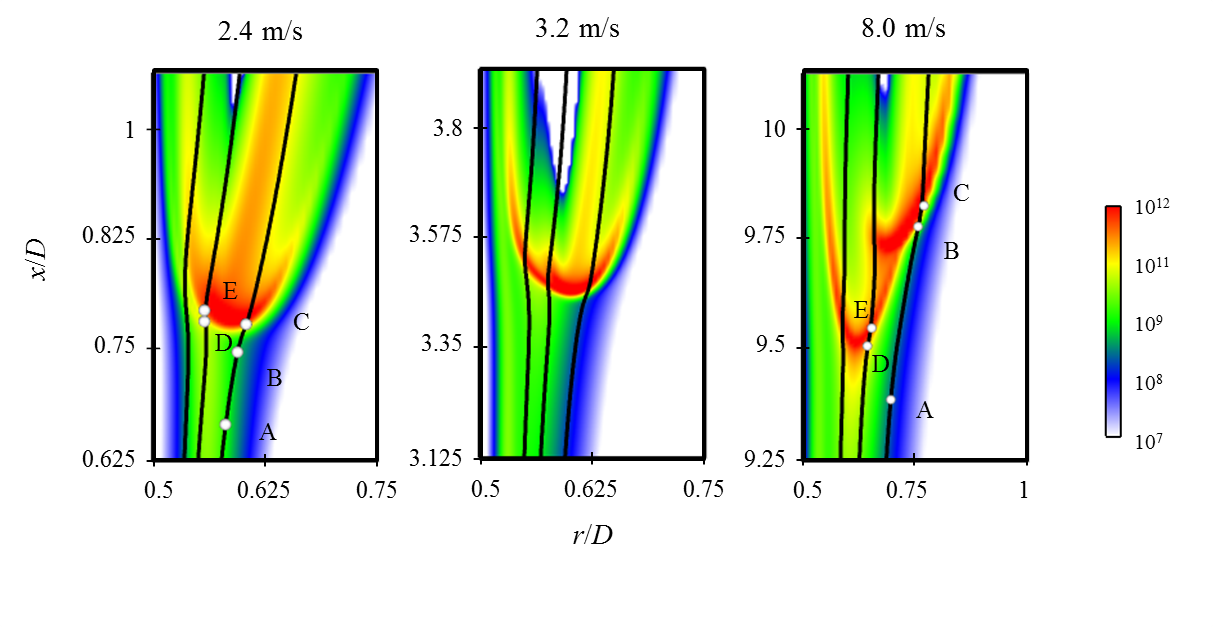
\includegraphics[width=1.0\textwidth]{ch-dynamics/HRR_V.png}
  \vspace{-0.3in}
  \normalsize
  \caption{Heat release rate [J/m$^3$-s] profiles for steady cases with the same boundary temperature but different flow velocities.  The iso-contours of $Z_{\rm st}$, $Z = 0.2$, and $Z = 0.3$ are outlined from right to left in solid lines, respectively.  The CEMA sampling points for $2.4$ and $8.0$ m/s cases are marked along the iso-contours.}
  \label{fig:HRR_V}
\end{figure}

When the inlet velocity is the lowest, $2.4$ m/s, a tribrachial thermal structure is observed very similar to that of the classical triple flame.  The triple point at $Z = 0.15$, where the three large heat release branches intersect, is also the stabilization point.  Some heat release can be found upstream of the tribrachial thermal structure for the partially reacting mixture at elevated temperature but is much less than the heat release from the flame structure.  As the inlet velocity increases to $3.2$ m/s, another branch with large heat release is found attached to the tribrachial structure around $Z = 0.2$.  The stabilization point is, again, the same as the triple point.  This structure has been analyzed in Sec.~\ref{sec:dynamics-T}.  However, as the inlet velocity further increases to $8.0$ m/s, the stabilization point is no longer on the tribrachial structure.  Instead, it is found to be near $Z = 0.25$ and is the intersection point of two trailing heat release branches.  Attached to the leaner branch, there is a tribrachial structure that appears similar to the triple flame structure.  This multibrachial structure is similar to the one discussed in Sec.~\ref{sec:dynamics-T} at a lower oxidizer temperature ($800$ K) and lower velocity ($3.2$ m/s).

Similar to Sec.~\ref{sec:diagnostics}, the controlling chemistry of the three cases was studied with CEMA.  Samplings were conducted along $Z_{\rm st}$, $Z = 0.2$, and $Z = 0.3$ iso-contours, as shown in Fig.~\ref{fig:HRR_V}.  Based on the explosive mode and participation index, the evolution of the dominant reactions is shown in Fig.~\ref{fig:CEMA_V}.

\begin{figure}
  \centering
  \scriptsize
  \resizebox{1.0\textwidth}{!}{% GNUPLOT: LaTeX picture with Postscript
\begingroup
  \makeatletter
  \providecommand\color[2][]{%
    \GenericError{(gnuplot) \space\space\space\@spaces}{%
      Package color not loaded in conjunction with
      terminal option `colourtext'%
    }{See the gnuplot documentation for explanation.%
    }{Either use 'blacktext' in gnuplot or load the package
      color.sty in LaTeX.}%
    \renewcommand\color[2][]{}%
  }%
  \providecommand\includegraphics[2][]{%
    \GenericError{(gnuplot) \space\space\space\@spaces}{%
      Package graphicx or graphics not loaded%
    }{See the gnuplot documentation for explanation.%
    }{The gnuplot epslatex terminal needs graphicx.sty or graphics.sty.}%
    \renewcommand\includegraphics[2][]{}%
  }%
  \providecommand\rotatebox[2]{#2}%
  \@ifundefined{ifGPcolor}{%
    \newif\ifGPcolor
    \GPcolortrue
  }{}%
  \@ifundefined{ifGPblacktext}{%
    \newif\ifGPblacktext
    \GPblacktexttrue
  }{}%
  % define a \g@addto@macro without @ in the name:
  \let\gplgaddtomacro\g@addto@macro
  % define empty templates for all commands taking text:
  \gdef\gplbacktext{}%
  \gdef\gplfronttext{}%
  \makeatother
  \ifGPblacktext
    % no textcolor at all
    \def\colorrgb#1{}%
    \def\colorgray#1{}%
  \else
    % gray or color?
    \ifGPcolor
      \def\colorrgb#1{\color[rgb]{#1}}%
      \def\colorgray#1{\color[gray]{#1}}%
      \expandafter\def\csname LTw\endcsname{\color{white}}%
      \expandafter\def\csname LTb\endcsname{\color{black}}%
      \expandafter\def\csname LTa\endcsname{\color{black}}%
      \expandafter\def\csname LT0\endcsname{\color[rgb]{1,0,0}}%
      \expandafter\def\csname LT1\endcsname{\color[rgb]{0,1,0}}%
      \expandafter\def\csname LT2\endcsname{\color[rgb]{0,0,1}}%
      \expandafter\def\csname LT3\endcsname{\color[rgb]{1,0,1}}%
      \expandafter\def\csname LT4\endcsname{\color[rgb]{0,1,1}}%
      \expandafter\def\csname LT5\endcsname{\color[rgb]{1,1,0}}%
      \expandafter\def\csname LT6\endcsname{\color[rgb]{0,0,0}}%
      \expandafter\def\csname LT7\endcsname{\color[rgb]{1,0.3,0}}%
      \expandafter\def\csname LT8\endcsname{\color[rgb]{0.5,0.5,0.5}}%
    \else
      % gray
      \def\colorrgb#1{\color{black}}%
      \def\colorgray#1{\color[gray]{#1}}%
      \expandafter\def\csname LTw\endcsname{\color{white}}%
      \expandafter\def\csname LTb\endcsname{\color{black}}%
      \expandafter\def\csname LTa\endcsname{\color{black}}%
      \expandafter\def\csname LT0\endcsname{\color{black}}%
      \expandafter\def\csname LT1\endcsname{\color{black}}%
      \expandafter\def\csname LT2\endcsname{\color{black}}%
      \expandafter\def\csname LT3\endcsname{\color{black}}%
      \expandafter\def\csname LT4\endcsname{\color{black}}%
      \expandafter\def\csname LT5\endcsname{\color{black}}%
      \expandafter\def\csname LT6\endcsname{\color{black}}%
      \expandafter\def\csname LT7\endcsname{\color{black}}%
      \expandafter\def\csname LT8\endcsname{\color{black}}%
    \fi
  \fi
  \setlength{\unitlength}{0.0500bp}%
  \begin{picture}(7200.00,5040.00)%
    \gplgaddtomacro\gplbacktext{%
      \csname LTb\endcsname%
      \put(2748,1043){\makebox(0,0)[r]{\strut{}CH$_3$OCH$_2$+O$_2$$\Longleftrightarrow$CH$_3$OCH$_2$O$_2$}}%
      \put(2748,1383){\makebox(0,0)[r]{\strut{}CH$_2$OCH$_2$O$_2$H$\Longleftrightarrow$OH+CH$_2$O+CH$_2$O}}%
      \put(2748,1722){\makebox(0,0)[r]{\strut{}CH$_3$OCH$_3$+OH$\Longleftrightarrow$CH$_3$OCH$_2$+H$_2$O}}%
      \put(2748,2061){\makebox(0,0)[r]{\strut{}H+O$_2$+M$\Longleftrightarrow$HO$_2$+M}}%
      \put(2748,2400){\makebox(0,0)[r]{\strut{}HCO+O$_2$$\Longleftrightarrow$CO+HO$_2$}}%
      \put(2748,2740){\makebox(0,0)[r]{\strut{}CH$_3$OCH$_2$O$_2$$\Longleftrightarrow$CH$_2$OCH$_2$O$_2$H}}%
      \put(2748,3079){\makebox(0,0)[r]{\strut{}CH$_2$O+OH$\Longleftrightarrow$HCO+H$_2$O}}%
      \put(2748,3418){\makebox(0,0)[r]{\strut{}HO$_2$CH$_2$OCHO$\Longleftrightarrow$OCH$_2$OCHO+OH}}%
      \put(2748,3757){\makebox(0,0)[r]{\strut{}CH$_2$O+H$\Longleftrightarrow$HCO+H$_2$}}%
      \put(2748,4097){\makebox(0,0)[r]{\strut{}CH$_3$OCH$_3$+H$\Longleftrightarrow$CH$_3$OCH$_2$+H$_2$}}%
      \put(2748,4436){\makebox(0,0)[r]{\strut{}H+O$_2$$\Longleftrightarrow$O+OH}}%
      \put(2880,484){\makebox(0,0){\strut{}-1}}%
      \put(3861,484){\makebox(0,0){\strut{}-0.5}}%
      \put(4842,484){\makebox(0,0){\strut{} 0}}%
      \put(5822,484){\makebox(0,0){\strut{} 0.5}}%
      \put(6803,484){\makebox(0,0){\strut{} 1}}%
      \csname LTb\endcsname%
      \put(4841,154){\makebox(0,0){\strut{}Normalized Participation Index}}%
      \put(5234,1332){\makebox(0,0)[l]{\strut{}Point A}}%
      \put(5234,1501){\makebox(0,0)[l]{\strut{}Point B}}%
      \put(5234,1688){\makebox(0,0)[l]{\strut{}Point C}}%
      \put(5234,1857){\makebox(0,0)[l]{\strut{}Point D}}%
      \put(5234,2027){\makebox(0,0)[l]{\strut{}Point E}}%
      \put(5234,2231){\makebox(0,0)[l]{\strut{}$2.4$ m/s}}%
    }%
    \gplgaddtomacro\gplfronttext{%
      \csname LTb\endcsname%
      \put(5690,1337){\makebox(0,0)[r]{\strut{} }}%
      \csname LTb\endcsname%
      \put(5690,1513){\makebox(0,0)[r]{\strut{} }}%
      \csname LTb\endcsname%
      \put(5690,1689){\makebox(0,0)[r]{\strut{} }}%
      \csname LTb\endcsname%
      \put(5690,1865){\makebox(0,0)[r]{\strut{} }}%
      \csname LTb\endcsname%
      \put(5690,2041){\makebox(0,0)[r]{\strut{} }}%
    }%
    \gplbacktext
    \put(0,0){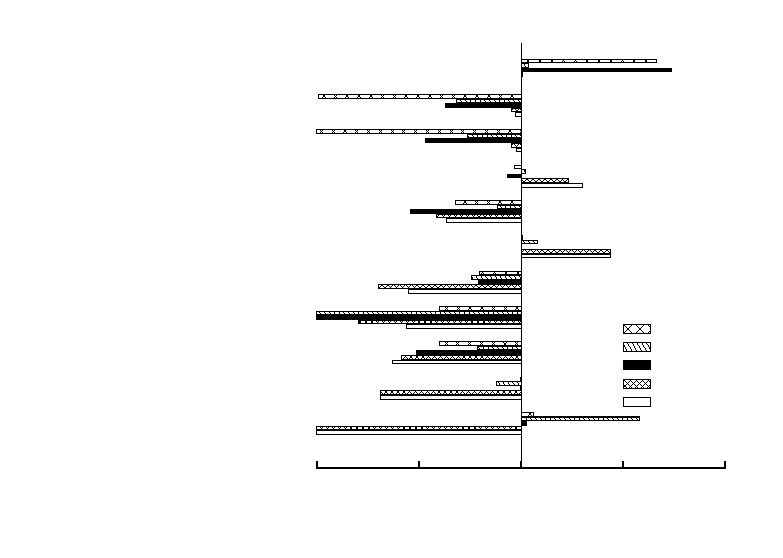
\includegraphics{ch-dynamics/CEMA_24}}%
    \gplfronttext
  \end{picture}%
\endgroup
}
  \resizebox{1.0\textwidth}{!}{% GNUPLOT: LaTeX picture with Postscript
\begingroup
  \makeatletter
  \providecommand\color[2][]{%
    \GenericError{(gnuplot) \space\space\space\@spaces}{%
      Package color not loaded in conjunction with
      terminal option `colourtext'%
    }{See the gnuplot documentation for explanation.%
    }{Either use 'blacktext' in gnuplot or load the package
      color.sty in LaTeX.}%
    \renewcommand\color[2][]{}%
  }%
  \providecommand\includegraphics[2][]{%
    \GenericError{(gnuplot) \space\space\space\@spaces}{%
      Package graphicx or graphics not loaded%
    }{See the gnuplot documentation for explanation.%
    }{The gnuplot epslatex terminal needs graphicx.sty or graphics.sty.}%
    \renewcommand\includegraphics[2][]{}%
  }%
  \providecommand\rotatebox[2]{#2}%
  \@ifundefined{ifGPcolor}{%
    \newif\ifGPcolor
    \GPcolortrue
  }{}%
  \@ifundefined{ifGPblacktext}{%
    \newif\ifGPblacktext
    \GPblacktexttrue
  }{}%
  % define a \g@addto@macro without @ in the name:
  \let\gplgaddtomacro\g@addto@macro
  % define empty templates for all commands taking text:
  \gdef\gplbacktext{}%
  \gdef\gplfronttext{}%
  \makeatother
  \ifGPblacktext
    % no textcolor at all
    \def\colorrgb#1{}%
    \def\colorgray#1{}%
  \else
    % gray or color?
    \ifGPcolor
      \def\colorrgb#1{\color[rgb]{#1}}%
      \def\colorgray#1{\color[gray]{#1}}%
      \expandafter\def\csname LTw\endcsname{\color{white}}%
      \expandafter\def\csname LTb\endcsname{\color{black}}%
      \expandafter\def\csname LTa\endcsname{\color{black}}%
      \expandafter\def\csname LT0\endcsname{\color[rgb]{1,0,0}}%
      \expandafter\def\csname LT1\endcsname{\color[rgb]{0,1,0}}%
      \expandafter\def\csname LT2\endcsname{\color[rgb]{0,0,1}}%
      \expandafter\def\csname LT3\endcsname{\color[rgb]{1,0,1}}%
      \expandafter\def\csname LT4\endcsname{\color[rgb]{0,1,1}}%
      \expandafter\def\csname LT5\endcsname{\color[rgb]{1,1,0}}%
      \expandafter\def\csname LT6\endcsname{\color[rgb]{0,0,0}}%
      \expandafter\def\csname LT7\endcsname{\color[rgb]{1,0.3,0}}%
      \expandafter\def\csname LT8\endcsname{\color[rgb]{0.5,0.5,0.5}}%
    \else
      % gray
      \def\colorrgb#1{\color{black}}%
      \def\colorgray#1{\color[gray]{#1}}%
      \expandafter\def\csname LTw\endcsname{\color{white}}%
      \expandafter\def\csname LTb\endcsname{\color{black}}%
      \expandafter\def\csname LTa\endcsname{\color{black}}%
      \expandafter\def\csname LT0\endcsname{\color{black}}%
      \expandafter\def\csname LT1\endcsname{\color{black}}%
      \expandafter\def\csname LT2\endcsname{\color{black}}%
      \expandafter\def\csname LT3\endcsname{\color{black}}%
      \expandafter\def\csname LT4\endcsname{\color{black}}%
      \expandafter\def\csname LT5\endcsname{\color{black}}%
      \expandafter\def\csname LT6\endcsname{\color{black}}%
      \expandafter\def\csname LT7\endcsname{\color{black}}%
      \expandafter\def\csname LT8\endcsname{\color{black}}%
    \fi
  \fi
  \setlength{\unitlength}{0.0500bp}%
  \begin{picture}(7200.00,5040.00)%
    \gplgaddtomacro\gplbacktext{%
      \csname LTb\endcsname%
      \put(2748,1043){\makebox(0,0)[r]{\strut{}H$_2$O$_2$+M$\Longleftrightarrow$OH+OH+M}}%
      \put(2748,1383){\makebox(0,0)[r]{\strut{}HCO+O$_2$$\Longleftrightarrow$CO+HO$_2$}}%
      \put(2748,1722){\makebox(0,0)[r]{\strut{}CH$_2$O+OH$\Longleftrightarrow$HCO+H$_2$O}}%
      \put(2748,2061){\makebox(0,0)[r]{\strut{}HO$_2$+HO$_2$$\Longleftrightarrow$H$_2$O$_2$+O$_2$}}%
      \put(2748,2400){\makebox(0,0)[r]{\strut{}CH$_3$OCH$_3$+HO$_2$$\Longleftrightarrow$CH$_3$OCH$_2$+H$_2$O$_2$}}%
      \put(2748,2740){\makebox(0,0)[r]{\strut{}CH$_3$OCH$_2$O$_2$$\Longleftrightarrow$CH$_2$OCH$_2$O$_2$H}}%
      \put(2748,3079){\makebox(0,0)[r]{\strut{}CH$_2$OCH$_2$O$_2$H$\Longleftrightarrow$OH+CH$_2$O+CH$_2$O}}%
      \put(2748,3418){\makebox(0,0)[r]{\strut{}CH$_3$OCH$_2$+O$_2$$\Longleftrightarrow$CH$_3$OCH$_2$O$_2$}}%
      \put(2748,3757){\makebox(0,0)[r]{\strut{}CH$_2$O+HO$_2$$\Longleftrightarrow$HCO+H$_2$O$_2$}}%
      \put(2748,4097){\makebox(0,0)[r]{\strut{}H+O$_2$+M$\Longleftrightarrow$HO$_2$+M}}%
      \put(2748,4436){\makebox(0,0)[r]{\strut{}H+O$_2$$\Longleftrightarrow$O+OH}}%
      \put(2880,484){\makebox(0,0){\strut{}-1}}%
      \put(3861,484){\makebox(0,0){\strut{}-0.5}}%
      \put(4842,484){\makebox(0,0){\strut{} 0}}%
      \put(5822,484){\makebox(0,0){\strut{} 0.5}}%
      \put(6803,484){\makebox(0,0){\strut{} 1}}%
      \csname LTb\endcsname%
      \put(4841,154){\makebox(0,0){\strut{}Normalized Participation Index}}%
      \put(5234,1332){\makebox(0,0)[l]{\strut{}Point A}}%
      \put(5234,1501){\makebox(0,0)[l]{\strut{}Point B}}%
      \put(5234,1688){\makebox(0,0)[l]{\strut{}Point C}}%
      \put(5234,1857){\makebox(0,0)[l]{\strut{}Point D}}%
      \put(5234,2027){\makebox(0,0)[l]{\strut{}Point E}}%
      \put(5234,2231){\makebox(0,0)[l]{\strut{}$8.0$ m/s}}%
    }%
    \gplgaddtomacro\gplfronttext{%
      \csname LTb\endcsname%
      \put(5690,1337){\makebox(0,0)[r]{\strut{} }}%
      \csname LTb\endcsname%
      \put(5690,1513){\makebox(0,0)[r]{\strut{} }}%
      \csname LTb\endcsname%
      \put(5690,1689){\makebox(0,0)[r]{\strut{} }}%
      \csname LTb\endcsname%
      \put(5690,1865){\makebox(0,0)[r]{\strut{} }}%
      \csname LTb\endcsname%
      \put(5690,2041){\makebox(0,0)[r]{\strut{} }}%
    }%
    \gplbacktext
    \put(0,0){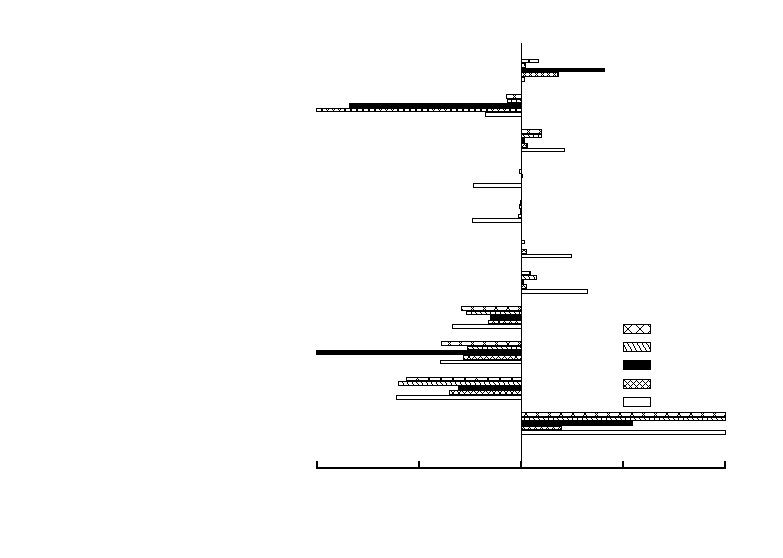
\includegraphics{ch-dynamics/CEMA_80}}%
    \gplfronttext
  \end{picture}%
\endgroup
}
  \normalsize
  \caption{Normalized participation index at $2.4$ and $8.0$ m/s.  Sampled locations are delineated in Fig.~\ref{fig:HRR_V}.}
  \label{fig:CEMA_V}
\end{figure}

At $2.4$ m/s, the dominant reactions along $Z_{\rm st}$ and $Z = 0.2$ iso-contours evolve in similar ways: upstream of the tribrachial structure (points A, B, and D), low-temperature chemistry, characterized by reactions involving CH$_3$OCH$_2$O$_2$ radicals, is active.  Due to the high diffusivity of H radicals and the elevated pressure, the H radical recombination reaction (H + O$_2$ + M $\Longleftrightarrow$ HO$_2$ + M) is important.  At the most reactive region (points C and E), the H radical branching reaction (H + O$_2$ $\Longleftrightarrow$ O + OH) becomes the most important chain branching reaction, indicating the transition to high-temperature chemistry.  On the contrary, for the $8.0$ m/s case, while low-temperature chemistry is still active upstream of the multibrachial structure, the dominant chain branching reaction is the hydrogen peroxide branching reaction (H$_2$O$_2$ + M $\Longleftrightarrow$ OH + OH + M).  Moreover, the dominant reactions along the $Z_{\rm st}$ and $Z = 0.2$ iso-contours evolve in different ways.  Along the $Z = 0.2$ iso-contour, from point D to E, the hydrogen peroxide branching reaction is always the dominant reaction, indicating the role of low-to-intermediate temperature autoignition chemistry~\cite{westbrook00}.  Although this is the case at point A on the $Z_{\rm st}$ iso-contour, the H radical chain branching reaction becomes dominant at point C, the most reactive zone, indicating that the dominant chemical pathway shifts to high-temperature chemistry.  CEMA results for the $3.2$ m/s case show similar transitions as those of the $8.0$ m/s case, although their thermal structures appear different.  Therefore, further computational diagnostics is needed to identify the dominant combustion mode.

\subsection{Stabilization Mechanism} 

Similar to the Lagrangian analysis presented in Sec.~\ref{sec:diagnostics}, the Lagrangian time history profiles of the two-dimensional computation and one-dimensional LFA are shown in Fig.~\ref{fig:LFA_V}.  For each inlet velocity case, the temperature profiles are compared along $Z_{\rm st}$, $Z = 0.2$, and $Z = 0.3$.

\begin{figure}
  \centering
  \scriptsize
  \resizebox{1.0\textwidth}{!}{% GNUPLOT: LaTeX picture with Postscript
\begingroup
  \makeatletter
  \providecommand\color[2][]{%
    \GenericError{(gnuplot) \space\space\space\@spaces}{%
      Package color not loaded in conjunction with
      terminal option `colourtext'%
    }{See the gnuplot documentation for explanation.%
    }{Either use 'blacktext' in gnuplot or load the package
      color.sty in LaTeX.}%
    \renewcommand\color[2][]{}%
  }%
  \providecommand\includegraphics[2][]{%
    \GenericError{(gnuplot) \space\space\space\@spaces}{%
      Package graphicx or graphics not loaded%
    }{See the gnuplot documentation for explanation.%
    }{The gnuplot epslatex terminal needs graphicx.sty or graphics.sty.}%
    \renewcommand\includegraphics[2][]{}%
  }%
  \providecommand\rotatebox[2]{#2}%
  \@ifundefined{ifGPcolor}{%
    \newif\ifGPcolor
    \GPcolortrue
  }{}%
  \@ifundefined{ifGPblacktext}{%
    \newif\ifGPblacktext
    \GPblacktexttrue
  }{}%
  % define a \g@addto@macro without @ in the name:
  \let\gplgaddtomacro\g@addto@macro
  % define empty templates for all commands taking text:
  \gdef\gplbacktext{}%
  \gdef\gplfronttext{}%
  \makeatother
  \ifGPblacktext
    % no textcolor at all
    \def\colorrgb#1{}%
    \def\colorgray#1{}%
  \else
    % gray or color?
    \ifGPcolor
      \def\colorrgb#1{\color[rgb]{#1}}%
      \def\colorgray#1{\color[gray]{#1}}%
      \expandafter\def\csname LTw\endcsname{\color{white}}%
      \expandafter\def\csname LTb\endcsname{\color{black}}%
      \expandafter\def\csname LTa\endcsname{\color{black}}%
      \expandafter\def\csname LT0\endcsname{\color[rgb]{1,0,0}}%
      \expandafter\def\csname LT1\endcsname{\color[rgb]{0,1,0}}%
      \expandafter\def\csname LT2\endcsname{\color[rgb]{0,0,1}}%
      \expandafter\def\csname LT3\endcsname{\color[rgb]{1,0,1}}%
      \expandafter\def\csname LT4\endcsname{\color[rgb]{0,1,1}}%
      \expandafter\def\csname LT5\endcsname{\color[rgb]{1,1,0}}%
      \expandafter\def\csname LT6\endcsname{\color[rgb]{0,0,0}}%
      \expandafter\def\csname LT7\endcsname{\color[rgb]{1,0.3,0}}%
      \expandafter\def\csname LT8\endcsname{\color[rgb]{0.5,0.5,0.5}}%
    \else
      % gray
      \def\colorrgb#1{\color{black}}%
      \def\colorgray#1{\color[gray]{#1}}%
      \expandafter\def\csname LTw\endcsname{\color{white}}%
      \expandafter\def\csname LTb\endcsname{\color{black}}%
      \expandafter\def\csname LTa\endcsname{\color{black}}%
      \expandafter\def\csname LT0\endcsname{\color{black}}%
      \expandafter\def\csname LT1\endcsname{\color{black}}%
      \expandafter\def\csname LT2\endcsname{\color{black}}%
      \expandafter\def\csname LT3\endcsname{\color{black}}%
      \expandafter\def\csname LT4\endcsname{\color{black}}%
      \expandafter\def\csname LT5\endcsname{\color{black}}%
      \expandafter\def\csname LT6\endcsname{\color{black}}%
      \expandafter\def\csname LT7\endcsname{\color{black}}%
      \expandafter\def\csname LT8\endcsname{\color{black}}%
    \fi
  \fi
  \setlength{\unitlength}{0.0500bp}%
  \begin{picture}(8640.00,6048.00)%
    \gplgaddtomacro\gplbacktext{%
      \csname LTb\endcsname%
      \put(6694,4756){\makebox(0,0)[r]{\strut{} 800}}%
      \put(6694,4961){\makebox(0,0)[r]{\strut{} 1200}}%
      \put(6694,5167){\makebox(0,0)[r]{\strut{} 1600}}%
      \put(6694,5372){\makebox(0,0)[r]{\strut{} 2000}}%
      \put(6694,5578){\makebox(0,0)[r]{\strut{} 2400}}%
      \put(6694,5783){\makebox(0,0)[r]{\strut{} 2800}}%
      \put(6826,4536){\makebox(0,0){\strut{} 0}}%
      \put(7137,4536){\makebox(0,0){\strut{} 0.5}}%
      \put(7448,4536){\makebox(0,0){\strut{} 1}}%
      \put(7759,4536){\makebox(0,0){\strut{} 1.5}}%
      \put(8070,4536){\makebox(0,0){\strut{} 2}}%
      \put(5792,5269){\rotatebox{-270}{\makebox(0,0){\strut{}\vspace{-36pt}$T$ [K]}}}%
      \put(7448,4206){\makebox(0,0){\strut{}\vspace{12pt}Time [ms]}}%
      \put(1987,6047){\makebox(0,0)[l]{\strut{}$2.4$ m/s}}%
      \put(4579,6047){\makebox(0,0)[l]{\strut{}$3.2$ m/s}}%
      \put(7170,6047){\makebox(0,0)[l]{\strut{}$8.0$ m/s}}%
      \put(-172,1633){\makebox(0,0)[l]{\strut{}$Z = 0.3$}}%
      \put(-172,3447){\makebox(0,0)[l]{\strut{}$Z = 0.2$}}%
      \put(-172,5261){\makebox(0,0)[l]{\strut{}$Z = Z_{\rm st}$}}%
    }%
    \gplgaddtomacro\gplfronttext{%
    }%
    \gplgaddtomacro\gplbacktext{%
      \csname LTb\endcsname%
      \put(6694,2941){\makebox(0,0)[r]{\strut{} 600}}%
      \put(6694,3147){\makebox(0,0)[r]{\strut{} 1000}}%
      \put(6694,3352){\makebox(0,0)[r]{\strut{} 1400}}%
      \put(6694,3558){\makebox(0,0)[r]{\strut{} 1800}}%
      \put(6694,3763){\makebox(0,0)[r]{\strut{} 2200}}%
      \put(6694,3969){\makebox(0,0)[r]{\strut{} 2600}}%
      \put(6826,2721){\makebox(0,0){\strut{} 0}}%
      \put(7137,2721){\makebox(0,0){\strut{} 0.5}}%
      \put(7448,2721){\makebox(0,0){\strut{} 1}}%
      \put(7759,2721){\makebox(0,0){\strut{} 1.5}}%
      \put(8070,2721){\makebox(0,0){\strut{} 2}}%
      \put(5792,3455){\rotatebox{-270}{\makebox(0,0){\strut{}\vspace{-36pt}$T$ [K]}}}%
      \put(7448,2391){\makebox(0,0){\strut{}\vspace{12pt}Time [ms]}}%
    }%
    \gplgaddtomacro\gplfronttext{%
    }%
    \gplgaddtomacro\gplbacktext{%
      \csname LTb\endcsname%
      \put(6694,1187){\makebox(0,0)[r]{\strut{} 400}}%
      \put(6694,1393){\makebox(0,0)[r]{\strut{} 800}}%
      \put(6694,1598){\makebox(0,0)[r]{\strut{} 1200}}%
      \put(6694,1804){\makebox(0,0)[r]{\strut{} 1600}}%
      \put(6694,2009){\makebox(0,0)[r]{\strut{} 2000}}%
      \put(6694,2215){\makebox(0,0)[r]{\strut{} 2400}}%
      \put(6826,967){\makebox(0,0){\strut{} 0}}%
      \put(7137,967){\makebox(0,0){\strut{} 0.5}}%
      \put(7448,967){\makebox(0,0){\strut{} 1}}%
      \put(7759,967){\makebox(0,0){\strut{} 1.5}}%
      \put(8070,967){\makebox(0,0){\strut{} 2}}%
      \put(5792,1701){\rotatebox{-270}{\makebox(0,0){\strut{}\vspace{-36pt}$T$ [K]}}}%
      \put(7448,637){\makebox(0,0){\strut{}\vspace{12pt}Time [ms]}}%
    }%
    \gplgaddtomacro\gplfronttext{%
    }%
    \gplgaddtomacro\gplbacktext{%
      \csname LTb\endcsname%
      \put(4102,4756){\makebox(0,0)[r]{\strut{} 800}}%
      \put(4102,4961){\makebox(0,0)[r]{\strut{} 1200}}%
      \put(4102,5167){\makebox(0,0)[r]{\strut{} 1600}}%
      \put(4102,5372){\makebox(0,0)[r]{\strut{} 2000}}%
      \put(4102,5578){\makebox(0,0)[r]{\strut{} 2400}}%
      \put(4102,5783){\makebox(0,0)[r]{\strut{} 2800}}%
      \put(4234,4536){\makebox(0,0){\strut{} 0}}%
      \put(4545,4536){\makebox(0,0){\strut{} 0.3}}%
      \put(4856,4536){\makebox(0,0){\strut{} 0.6}}%
      \put(5167,4536){\makebox(0,0){\strut{} 0.9}}%
      \put(5478,4536){\makebox(0,0){\strut{} 1.2}}%
      \put(3200,5269){\rotatebox{-270}{\makebox(0,0){\strut{}\vspace{-36pt}$T$ [K]}}}%
      \put(4856,4206){\makebox(0,0){\strut{}\vspace{12pt}Time [ms]}}%
    }%
    \gplgaddtomacro\gplfronttext{%
    }%
    \gplgaddtomacro\gplbacktext{%
      \csname LTb\endcsname%
      \put(4102,2941){\makebox(0,0)[r]{\strut{} 600}}%
      \put(4102,3147){\makebox(0,0)[r]{\strut{} 1000}}%
      \put(4102,3352){\makebox(0,0)[r]{\strut{} 1400}}%
      \put(4102,3558){\makebox(0,0)[r]{\strut{} 1800}}%
      \put(4102,3763){\makebox(0,0)[r]{\strut{} 2200}}%
      \put(4102,3969){\makebox(0,0)[r]{\strut{} 2600}}%
      \put(4234,2721){\makebox(0,0){\strut{} 0}}%
      \put(4545,2721){\makebox(0,0){\strut{} 0.3}}%
      \put(4856,2721){\makebox(0,0){\strut{} 0.6}}%
      \put(5167,2721){\makebox(0,0){\strut{} 0.9}}%
      \put(5478,2721){\makebox(0,0){\strut{} 1.2}}%
      \put(3200,3455){\rotatebox{-270}{\makebox(0,0){\strut{}\vspace{-36pt}$T$ [K]}}}%
      \put(4856,2391){\makebox(0,0){\strut{}\vspace{12pt}Time [ms]}}%
    }%
    \gplgaddtomacro\gplfronttext{%
    }%
    \gplgaddtomacro\gplbacktext{%
      \csname LTb\endcsname%
      \put(4102,1187){\makebox(0,0)[r]{\strut{} 400}}%
      \put(4102,1393){\makebox(0,0)[r]{\strut{} 800}}%
      \put(4102,1598){\makebox(0,0)[r]{\strut{} 1200}}%
      \put(4102,1804){\makebox(0,0)[r]{\strut{} 1600}}%
      \put(4102,2009){\makebox(0,0)[r]{\strut{} 2000}}%
      \put(4102,2215){\makebox(0,0)[r]{\strut{} 2400}}%
      \put(4234,967){\makebox(0,0){\strut{} 0}}%
      \put(4545,967){\makebox(0,0){\strut{} 0.3}}%
      \put(4856,967){\makebox(0,0){\strut{} 0.6}}%
      \put(5167,967){\makebox(0,0){\strut{} 0.9}}%
      \put(5478,967){\makebox(0,0){\strut{} 1.2}}%
      \put(3200,1701){\rotatebox{-270}{\makebox(0,0){\strut{}\vspace{-36pt}$T$ [K]}}}%
      \put(4856,637){\makebox(0,0){\strut{}\vspace{12pt}Time [ms]}}%
    }%
    \gplgaddtomacro\gplfronttext{%
    }%
    \gplgaddtomacro\gplbacktext{%
      \csname LTb\endcsname%
      \put(1510,4756){\makebox(0,0)[r]{\strut{} 800}}%
      \put(1510,4961){\makebox(0,0)[r]{\strut{} 1200}}%
      \put(1510,5167){\makebox(0,0)[r]{\strut{} 1600}}%
      \put(1510,5372){\makebox(0,0)[r]{\strut{} 2000}}%
      \put(1510,5578){\makebox(0,0)[r]{\strut{} 2400}}%
      \put(1510,5783){\makebox(0,0)[r]{\strut{} 2800}}%
      \put(1642,4536){\makebox(0,0){\strut{} 0}}%
      \put(1953,4536){\makebox(0,0){\strut{} 0.3}}%
      \put(2264,4536){\makebox(0,0){\strut{} 0.6}}%
      \put(2575,4536){\makebox(0,0){\strut{} 0.9}}%
      \put(2886,4536){\makebox(0,0){\strut{} 1.2}}%
      \put(608,5269){\rotatebox{-270}{\makebox(0,0){\strut{}\vspace{-36pt}$T$ [K]}}}%
      \put(2264,4206){\makebox(0,0){\strut{}\vspace{12pt}Time [ms]}}%
    }%
    \gplgaddtomacro\gplfronttext{%
    }%
    \gplgaddtomacro\gplbacktext{%
      \csname LTb\endcsname%
      \put(1510,2941){\makebox(0,0)[r]{\strut{} 600}}%
      \put(1510,3147){\makebox(0,0)[r]{\strut{} 1000}}%
      \put(1510,3352){\makebox(0,0)[r]{\strut{} 1400}}%
      \put(1510,3558){\makebox(0,0)[r]{\strut{} 1800}}%
      \put(1510,3763){\makebox(0,0)[r]{\strut{} 2200}}%
      \put(1510,3969){\makebox(0,0)[r]{\strut{} 2600}}%
      \put(1642,2721){\makebox(0,0){\strut{} 0}}%
      \put(1953,2721){\makebox(0,0){\strut{} 0.3}}%
      \put(2264,2721){\makebox(0,0){\strut{} 0.6}}%
      \put(2575,2721){\makebox(0,0){\strut{} 0.9}}%
      \put(2886,2721){\makebox(0,0){\strut{} 1.2}}%
      \put(608,3455){\rotatebox{-270}{\makebox(0,0){\strut{}\vspace{-36pt}$T$ [K]}}}%
      \put(2264,2391){\makebox(0,0){\strut{}\vspace{12pt}Time [ms]}}%
    }%
    \gplgaddtomacro\gplfronttext{%
    }%
    \gplgaddtomacro\gplbacktext{%
      \csname LTb\endcsname%
      \put(1510,1187){\makebox(0,0)[r]{\strut{} 400}}%
      \put(1510,1393){\makebox(0,0)[r]{\strut{} 800}}%
      \put(1510,1598){\makebox(0,0)[r]{\strut{} 1200}}%
      \put(1510,1804){\makebox(0,0)[r]{\strut{} 1600}}%
      \put(1510,2009){\makebox(0,0)[r]{\strut{} 2000}}%
      \put(1510,2215){\makebox(0,0)[r]{\strut{} 2400}}%
      \put(1642,967){\makebox(0,0){\strut{} 0}}%
      \put(1953,967){\makebox(0,0){\strut{} 0.3}}%
      \put(2264,967){\makebox(0,0){\strut{} 0.6}}%
      \put(2575,967){\makebox(0,0){\strut{} 0.9}}%
      \put(2886,967){\makebox(0,0){\strut{} 1.2}}%
      \put(608,1701){\rotatebox{-270}{\makebox(0,0){\strut{}\vspace{-36pt}$T$ [K]}}}%
      \put(2264,637){\makebox(0,0){\strut{}\vspace{12pt}Time [ms]}}%
      \put(4147,242){\makebox(0,0)[l]{\strut{}2D-CFD}}%
      \put(5270,242){\makebox(0,0)[l]{\strut{}1D-LFA}}%
    }%
    \gplgaddtomacro\gplfronttext{%
      \csname LTb\endcsname%
      \put(3646,253){\makebox(0,0)[r]{\strut{} }}%
      \csname LTb\endcsname%
      \put(4765,253){\makebox(0,0)[r]{\strut{}    }}%
    }%
    \gplbacktext
    \put(0,0){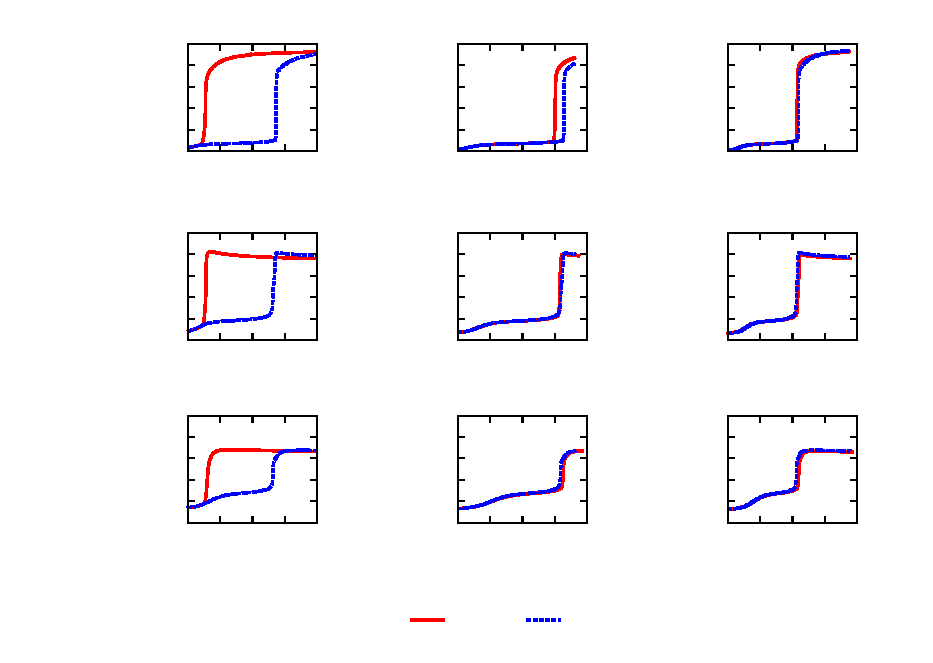
\includegraphics{ch-dynamics/LFA_V}}%
    \gplfronttext
  \end{picture}%
\endgroup
}
  \normalsize
  \caption{Comparison between 2D-CFD and 1D-LFA results for the steady cases with the same boundary temperature but different flow velocities.}
  \label{fig:LFA_V}
\end{figure}

For the $2.4$ m/s case, LFA fails to match the two-dimensional result at all three mixture fractions, indicating that transport processes normal to the mixture fraction gradient are crucial, which further indicates that flame propagation is the dominant stabilization mechanism.  At $3.2$ m/s, LFA slightly lags behind the two-dimensional result at $Z_{\rm st}$ but matches well at $Z = 0.2$ and $Z = 0.3$.  Recalling the heat release profile in Fig.~\ref{fig:HRR_V}, these results indicate that the tetrabrachial structure consists of a tribrachial structure, at which flame propagation is not negligible, and the richer branch that intersects with the tribrachial flame is an autoignition front, whose response is well captured with the one-dimensional flamelet model.  As a result, stabilization of the $3.2$ m/s case is characterized as a mixed mode of inhomogeneous autoignition and premixed flame propagation, depending on the local mixture fraction.  At $8.0$ m/s, LFA agrees well with the two-dimensional result at all mixture fractions, indicating that the transport processes normal to the mixture fraction gradient are negligible.  Therefore, the stabilization mechanism is characterized as inhomogeneous autoignition.

\subsection{Autoignition and Flame Interaction}

As shown by LFA, under some conditions, inhomogeneous autoignition and premixed flame propagation both contribute to flame stabilization, resulting in a multimode stabilized regime.  Furthermore, the interaction between autoignition and flame propagation is tightly coupled.  If the thermal structure is mainly \emph{kinetically} stabilized, heat and radicals generated by autoignition will modify the  downstream thermal and chemical environment and thus the local flame speed.  On the contrary, if stabilization is mainly \emph{kinematic} in nature then heat and radicals generated by the flame can back diffuse upstream, modifying the reactivity upstream.  

To demonstrate these complex interactions and understand the transition between \emph{kinetic} and \emph{kinematic} stabilization mechanisms, the LFA results for the $2.4$ m/s case were further analyzed.  As shown in Fig.~\ref{fig:LFA_V}, if there was a \emph{kinetically} stabilized inhomogeneous autoignition front, this front would stabilize further downstream than the \emph{kinematically} stabilized flame front.  Although not shown, CEMA of these LFA solutions show the same evolution of the controlling chemistry as the $8.0$ m/s case.  In particular, the low-to-intermediate temperature hydrogen peroxide chain branching reaction dominates the transition to autoignition.  Therefore, the nature and the qualitative structures of the inhomogeneous autoignition fronts, as predicted by LFA in Fig.~\ref{fig:LFA_V} for the two lower inlet velocity cases, are essentially the same as the $8.0$ m/s case.  

A general description of the initiation of these multibrachial inhomogeneous autoignition fronts in all three cases is that, due to radical accumulation and heat release, the controlling chemistry shifts from low-temperature chemistry, represented by CH$_3$OCH$_2$O$_2$ reactions, to hydrogen peroxide branching reactions.  At some mixture fractions, higher temperatures and more oxidizer supply enable the dominant chemistry to transition further to high-temperature chemistry, as characterized by the H radical branching reaction.  As shown in Fig.~\ref{fig:1D_V}, there are double or triple heat release peaks, depending on the mixture fraction.  However, for all mixture fractions, these peaks correlate very well with the inflection points on the temperature profiles and peaks on the OH radical profiles.  Comparing them with the CH$_3$OCH$_2$O$_2$ radical profile, it is clear that low-temperature chemistry results in the first peak of heat release profile and produces OH radicals.  Hydrogen peroxide accumulates until it decomposes at the second heat release peak and produces OH radicals through H$_2$O$_2$ + M $\Longleftrightarrow$ OH + OH + M.  At $Z_{\rm st}$ and $Z = 0.2$, there is a third heat release and OH radical peak, which is due to the H + O$_2$ $\Longleftrightarrow$ O + OH reaction.  At $Z_{\rm st}$, the second and third peaks appear to be much closer compared with those at $Z = 0.2$, probably due to higher temperature and more abundant oxidizer, such that the H radical chain branching reaction is activated earlier.  Due to the lack of oxidizer, the third peak is not observed at $Z = 0.3$.  

\begin{figure}
  \vspace{-1in}
  \centering
  \scriptsize
  % GNUPLOT: LaTeX picture with Postscript
\begingroup
  \makeatletter
  \providecommand\color[2][]{%
    \GenericError{(gnuplot) \space\space\space\@spaces}{%
      Package color not loaded in conjunction with
      terminal option `colourtext'%
    }{See the gnuplot documentation for explanation.%
    }{Either use 'blacktext' in gnuplot or load the package
      color.sty in LaTeX.}%
    \renewcommand\color[2][]{}%
  }%
  \providecommand\includegraphics[2][]{%
    \GenericError{(gnuplot) \space\space\space\@spaces}{%
      Package graphicx or graphics not loaded%
    }{See the gnuplot documentation for explanation.%
    }{The gnuplot epslatex terminal needs graphicx.sty or graphics.sty.}%
    \renewcommand\includegraphics[2][]{}%
  }%
  \providecommand\rotatebox[2]{#2}%
  \@ifundefined{ifGPcolor}{%
    \newif\ifGPcolor
    \GPcolortrue
  }{}%
  \@ifundefined{ifGPblacktext}{%
    \newif\ifGPblacktext
    \GPblacktexttrue
  }{}%
  % define a \g@addto@macro without @ in the name:
  \let\gplgaddtomacro\g@addto@macro
  % define empty templates for all commands taking text:
  \gdef\gplbacktext{}%
  \gdef\gplfronttext{}%
  \makeatother
  \ifGPblacktext
    % no textcolor at all
    \def\colorrgb#1{}%
    \def\colorgray#1{}%
  \else
    % gray or color?
    \ifGPcolor
      \def\colorrgb#1{\color[rgb]{#1}}%
      \def\colorgray#1{\color[gray]{#1}}%
      \expandafter\def\csname LTw\endcsname{\color{white}}%
      \expandafter\def\csname LTb\endcsname{\color{black}}%
      \expandafter\def\csname LTa\endcsname{\color{black}}%
      \expandafter\def\csname LT0\endcsname{\color[rgb]{1,0,0}}%
      \expandafter\def\csname LT1\endcsname{\color[rgb]{0,1,0}}%
      \expandafter\def\csname LT2\endcsname{\color[rgb]{0,0,1}}%
      \expandafter\def\csname LT3\endcsname{\color[rgb]{1,0,1}}%
      \expandafter\def\csname LT4\endcsname{\color[rgb]{0,1,1}}%
      \expandafter\def\csname LT5\endcsname{\color[rgb]{1,1,0}}%
      \expandafter\def\csname LT6\endcsname{\color[rgb]{0,0,0}}%
      \expandafter\def\csname LT7\endcsname{\color[rgb]{1,0.3,0}}%
      \expandafter\def\csname LT8\endcsname{\color[rgb]{0.5,0.5,0.5}}%
    \else
      % gray
      \def\colorrgb#1{\color{black}}%
      \def\colorgray#1{\color[gray]{#1}}%
      \expandafter\def\csname LTw\endcsname{\color{white}}%
      \expandafter\def\csname LTb\endcsname{\color{black}}%
      \expandafter\def\csname LTa\endcsname{\color{black}}%
      \expandafter\def\csname LT0\endcsname{\color{black}}%
      \expandafter\def\csname LT1\endcsname{\color{black}}%
      \expandafter\def\csname LT2\endcsname{\color{black}}%
      \expandafter\def\csname LT3\endcsname{\color{black}}%
      \expandafter\def\csname LT4\endcsname{\color{black}}%
      \expandafter\def\csname LT5\endcsname{\color{black}}%
      \expandafter\def\csname LT6\endcsname{\color{black}}%
      \expandafter\def\csname LT7\endcsname{\color{black}}%
      \expandafter\def\csname LT8\endcsname{\color{black}}%
    \fi
  \fi
  \setlength{\unitlength}{0.0500bp}%
  \begin{picture}(5760.00,2520.00)%
    \gplgaddtomacro\gplbacktext{%
      \csname LTb\endcsname%
      \put(1342,440){\makebox(0,0)[r]{\strut{}1.0e+08}}%
      \put(1342,1045){\makebox(0,0)[r]{\strut{}1.0e+10}}%
      \put(1342,1651){\makebox(0,0)[r]{\strut{}1.0e+12}}%
      \put(1342,2256){\makebox(0,0)[r]{\strut{}1.0e+14}}%
      \put(1474,220){\makebox(0,0){\strut{} 0}}%
      \put(2446,220){\makebox(0,0){\strut{} 0.3}}%
      \put(3419,220){\makebox(0,0){\strut{} 0.6}}%
      \put(4391,220){\makebox(0,0){\strut{} 0.9}}%
      \put(5363,220){\makebox(0,0){\strut{} 1.2}}%
      \put(176,1348){\rotatebox{-270}{\makebox(0,0){\strut{}\vspace{-28pt}$HRR$ [J/m$^3$-s]}}}%
    }%
    \gplgaddtomacro\gplfronttext{%
      \csname LTb\endcsname%
      \put(2530,2083){\makebox(0,0)[r]{\strut{}$Z_{\rm st}$}}%
      \csname LTb\endcsname%
      \put(2530,1863){\makebox(0,0)[r]{\strut{}$Z = 0.2$}}%
      \csname LTb\endcsname%
      \put(2530,1643){\makebox(0,0)[r]{\strut{}$Z = 0.3$}}%
    }%
    \gplbacktext
    \put(0,0){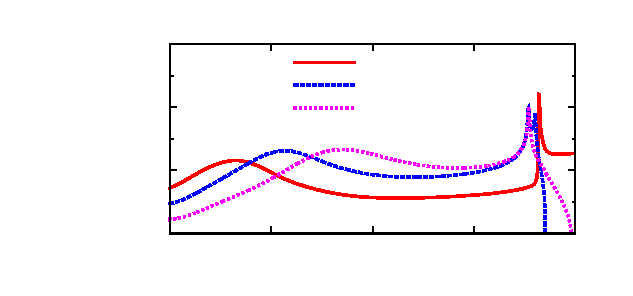
\includegraphics{1D_V_HRR}}%
    \gplfronttext
  \end{picture}%
\endgroup

  % GNUPLOT: LaTeX picture with Postscript
\begingroup
  \makeatletter
  \providecommand\color[2][]{%
    \GenericError{(gnuplot) \space\space\space\@spaces}{%
      Package color not loaded in conjunction with
      terminal option `colourtext'%
    }{See the gnuplot documentation for explanation.%
    }{Either use 'blacktext' in gnuplot or load the package
      color.sty in LaTeX.}%
    \renewcommand\color[2][]{}%
  }%
  \providecommand\includegraphics[2][]{%
    \GenericError{(gnuplot) \space\space\space\@spaces}{%
      Package graphicx or graphics not loaded%
    }{See the gnuplot documentation for explanation.%
    }{The gnuplot epslatex terminal needs graphicx.sty or graphics.sty.}%
    \renewcommand\includegraphics[2][]{}%
  }%
  \providecommand\rotatebox[2]{#2}%
  \@ifundefined{ifGPcolor}{%
    \newif\ifGPcolor
    \GPcolortrue
  }{}%
  \@ifundefined{ifGPblacktext}{%
    \newif\ifGPblacktext
    \GPblacktexttrue
  }{}%
  % define a \g@addto@macro without @ in the name:
  \let\gplgaddtomacro\g@addto@macro
  % define empty templates for all commands taking text:
  \gdef\gplbacktext{}%
  \gdef\gplfronttext{}%
  \makeatother
  \ifGPblacktext
    % no textcolor at all
    \def\colorrgb#1{}%
    \def\colorgray#1{}%
  \else
    % gray or color?
    \ifGPcolor
      \def\colorrgb#1{\color[rgb]{#1}}%
      \def\colorgray#1{\color[gray]{#1}}%
      \expandafter\def\csname LTw\endcsname{\color{white}}%
      \expandafter\def\csname LTb\endcsname{\color{black}}%
      \expandafter\def\csname LTa\endcsname{\color{black}}%
      \expandafter\def\csname LT0\endcsname{\color[rgb]{1,0,0}}%
      \expandafter\def\csname LT1\endcsname{\color[rgb]{0,1,0}}%
      \expandafter\def\csname LT2\endcsname{\color[rgb]{0,0,1}}%
      \expandafter\def\csname LT3\endcsname{\color[rgb]{1,0,1}}%
      \expandafter\def\csname LT4\endcsname{\color[rgb]{0,1,1}}%
      \expandafter\def\csname LT5\endcsname{\color[rgb]{1,1,0}}%
      \expandafter\def\csname LT6\endcsname{\color[rgb]{0,0,0}}%
      \expandafter\def\csname LT7\endcsname{\color[rgb]{1,0.3,0}}%
      \expandafter\def\csname LT8\endcsname{\color[rgb]{0.5,0.5,0.5}}%
    \else
      % gray
      \def\colorrgb#1{\color{black}}%
      \def\colorgray#1{\color[gray]{#1}}%
      \expandafter\def\csname LTw\endcsname{\color{white}}%
      \expandafter\def\csname LTb\endcsname{\color{black}}%
      \expandafter\def\csname LTa\endcsname{\color{black}}%
      \expandafter\def\csname LT0\endcsname{\color{black}}%
      \expandafter\def\csname LT1\endcsname{\color{black}}%
      \expandafter\def\csname LT2\endcsname{\color{black}}%
      \expandafter\def\csname LT3\endcsname{\color{black}}%
      \expandafter\def\csname LT4\endcsname{\color{black}}%
      \expandafter\def\csname LT5\endcsname{\color{black}}%
      \expandafter\def\csname LT6\endcsname{\color{black}}%
      \expandafter\def\csname LT7\endcsname{\color{black}}%
      \expandafter\def\csname LT8\endcsname{\color{black}}%
    \fi
  \fi
  \setlength{\unitlength}{0.0500bp}%
  \begin{picture}(5760.00,2520.00)%
    \gplgaddtomacro\gplbacktext{%
      \csname LTb\endcsname%
      \put(1342,440){\makebox(0,0)[r]{\strut{}5.0e+02}}%
      \put(1342,1045){\makebox(0,0)[r]{\strut{}1.2e+03}}%
      \put(1342,1651){\makebox(0,0)[r]{\strut{}1.9e+03}}%
      \put(1342,2256){\makebox(0,0)[r]{\strut{}2.6e+03}}%
      \put(1474,220){\makebox(0,0){\strut{} 0}}%
      \put(2446,220){\makebox(0,0){\strut{} 0.3}}%
      \put(3419,220){\makebox(0,0){\strut{} 0.6}}%
      \put(4391,220){\makebox(0,0){\strut{} 0.9}}%
      \put(5363,220){\makebox(0,0){\strut{} 1.2}}%
      \put(176,1348){\rotatebox{-270}{\makebox(0,0){\strut{}\vspace{-28pt}$T$ [K]}}}%
    }%
    \gplgaddtomacro\gplfronttext{%
      \csname LTb\endcsname%
      \put(2530,2083){\makebox(0,0)[r]{\strut{}$Z_{\rm st}$}}%
      \csname LTb\endcsname%
      \put(2530,1863){\makebox(0,0)[r]{\strut{}$Z = 0.2$}}%
      \csname LTb\endcsname%
      \put(2530,1643){\makebox(0,0)[r]{\strut{}$Z = 0.3$}}%
    }%
    \gplbacktext
    \put(0,0){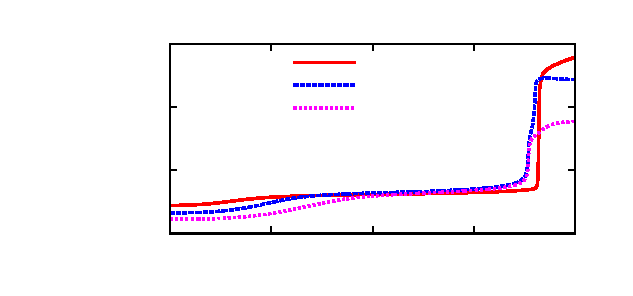
\includegraphics{ch-dynamics/1D_V_T}}%
    \gplfronttext
  \end{picture}%
\endgroup

  % GNUPLOT: LaTeX picture with Postscript
\begingroup
  \makeatletter
  \providecommand\color[2][]{%
    \GenericError{(gnuplot) \space\space\space\@spaces}{%
      Package color not loaded in conjunction with
      terminal option `colourtext'%
    }{See the gnuplot documentation for explanation.%
    }{Either use 'blacktext' in gnuplot or load the package
      color.sty in LaTeX.}%
    \renewcommand\color[2][]{}%
  }%
  \providecommand\includegraphics[2][]{%
    \GenericError{(gnuplot) \space\space\space\@spaces}{%
      Package graphicx or graphics not loaded%
    }{See the gnuplot documentation for explanation.%
    }{The gnuplot epslatex terminal needs graphicx.sty or graphics.sty.}%
    \renewcommand\includegraphics[2][]{}%
  }%
  \providecommand\rotatebox[2]{#2}%
  \@ifundefined{ifGPcolor}{%
    \newif\ifGPcolor
    \GPcolortrue
  }{}%
  \@ifundefined{ifGPblacktext}{%
    \newif\ifGPblacktext
    \GPblacktexttrue
  }{}%
  % define a \g@addto@macro without @ in the name:
  \let\gplgaddtomacro\g@addto@macro
  % define empty templates for all commands taking text:
  \gdef\gplbacktext{}%
  \gdef\gplfronttext{}%
  \makeatother
  \ifGPblacktext
    % no textcolor at all
    \def\colorrgb#1{}%
    \def\colorgray#1{}%
  \else
    % gray or color?
    \ifGPcolor
      \def\colorrgb#1{\color[rgb]{#1}}%
      \def\colorgray#1{\color[gray]{#1}}%
      \expandafter\def\csname LTw\endcsname{\color{white}}%
      \expandafter\def\csname LTb\endcsname{\color{black}}%
      \expandafter\def\csname LTa\endcsname{\color{black}}%
      \expandafter\def\csname LT0\endcsname{\color[rgb]{1,0,0}}%
      \expandafter\def\csname LT1\endcsname{\color[rgb]{0,1,0}}%
      \expandafter\def\csname LT2\endcsname{\color[rgb]{0,0,1}}%
      \expandafter\def\csname LT3\endcsname{\color[rgb]{1,0,1}}%
      \expandafter\def\csname LT4\endcsname{\color[rgb]{0,1,1}}%
      \expandafter\def\csname LT5\endcsname{\color[rgb]{1,1,0}}%
      \expandafter\def\csname LT6\endcsname{\color[rgb]{0,0,0}}%
      \expandafter\def\csname LT7\endcsname{\color[rgb]{1,0.3,0}}%
      \expandafter\def\csname LT8\endcsname{\color[rgb]{0.5,0.5,0.5}}%
    \else
      % gray
      \def\colorrgb#1{\color{black}}%
      \def\colorgray#1{\color[gray]{#1}}%
      \expandafter\def\csname LTw\endcsname{\color{white}}%
      \expandafter\def\csname LTb\endcsname{\color{black}}%
      \expandafter\def\csname LTa\endcsname{\color{black}}%
      \expandafter\def\csname LT0\endcsname{\color{black}}%
      \expandafter\def\csname LT1\endcsname{\color{black}}%
      \expandafter\def\csname LT2\endcsname{\color{black}}%
      \expandafter\def\csname LT3\endcsname{\color{black}}%
      \expandafter\def\csname LT4\endcsname{\color{black}}%
      \expandafter\def\csname LT5\endcsname{\color{black}}%
      \expandafter\def\csname LT6\endcsname{\color{black}}%
      \expandafter\def\csname LT7\endcsname{\color{black}}%
      \expandafter\def\csname LT8\endcsname{\color{black}}%
    \fi
  \fi
  \setlength{\unitlength}{0.0500bp}%
  \begin{picture}(5760.00,2520.00)%
    \gplgaddtomacro\gplbacktext{%
      \csname LTb\endcsname%
      \put(1342,440){\makebox(0,0)[r]{\strut{}1.0e-08}}%
      \put(1342,1045){\makebox(0,0)[r]{\strut{}1.0e-06}}%
      \put(1342,1651){\makebox(0,0)[r]{\strut{}1.0e-04}}%
      \put(1342,2256){\makebox(0,0)[r]{\strut{}1.0e-02}}%
      \put(1474,220){\makebox(0,0){\strut{} 0}}%
      \put(2446,220){\makebox(0,0){\strut{} 0.3}}%
      \put(3419,220){\makebox(0,0){\strut{} 0.6}}%
      \put(4391,220){\makebox(0,0){\strut{} 0.9}}%
      \put(5363,220){\makebox(0,0){\strut{} 1.2}}%
      \put(176,1348){\rotatebox{-270}{\makebox(0,0){\strut{}\vspace{-28pt}OH Mass Fraction}}}%
    }%
    \gplgaddtomacro\gplfronttext{%
      \csname LTb\endcsname%
      \put(2530,2083){\makebox(0,0)[r]{\strut{}$Z_{\rm st}$}}%
      \csname LTb\endcsname%
      \put(2530,1863){\makebox(0,0)[r]{\strut{}$Z = 0.2$}}%
      \csname LTb\endcsname%
      \put(2530,1643){\makebox(0,0)[r]{\strut{}$Z = 0.3$}}%
    }%
    \gplbacktext
    \put(0,0){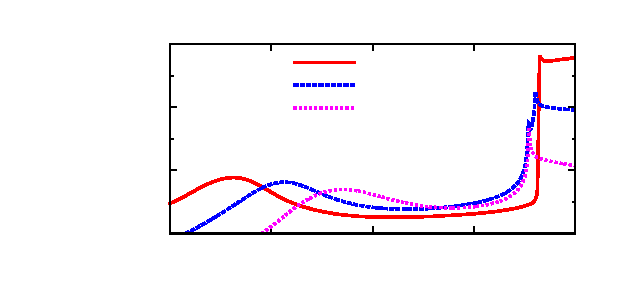
\includegraphics{1D_V_OH}}%
    \gplfronttext
  \end{picture}%
\endgroup

  % GNUPLOT: LaTeX picture with Postscript
\begingroup
  \makeatletter
  \providecommand\color[2][]{%
    \GenericError{(gnuplot) \space\space\space\@spaces}{%
      Package color not loaded in conjunction with
      terminal option `colourtext'%
    }{See the gnuplot documentation for explanation.%
    }{Either use 'blacktext' in gnuplot or load the package
      color.sty in LaTeX.}%
    \renewcommand\color[2][]{}%
  }%
  \providecommand\includegraphics[2][]{%
    \GenericError{(gnuplot) \space\space\space\@spaces}{%
      Package graphicx or graphics not loaded%
    }{See the gnuplot documentation for explanation.%
    }{The gnuplot epslatex terminal needs graphicx.sty or graphics.sty.}%
    \renewcommand\includegraphics[2][]{}%
  }%
  \providecommand\rotatebox[2]{#2}%
  \@ifundefined{ifGPcolor}{%
    \newif\ifGPcolor
    \GPcolortrue
  }{}%
  \@ifundefined{ifGPblacktext}{%
    \newif\ifGPblacktext
    \GPblacktexttrue
  }{}%
  % define a \g@addto@macro without @ in the name:
  \let\gplgaddtomacro\g@addto@macro
  % define empty templates for all commands taking text:
  \gdef\gplbacktext{}%
  \gdef\gplfronttext{}%
  \makeatother
  \ifGPblacktext
    % no textcolor at all
    \def\colorrgb#1{}%
    \def\colorgray#1{}%
  \else
    % gray or color?
    \ifGPcolor
      \def\colorrgb#1{\color[rgb]{#1}}%
      \def\colorgray#1{\color[gray]{#1}}%
      \expandafter\def\csname LTw\endcsname{\color{white}}%
      \expandafter\def\csname LTb\endcsname{\color{black}}%
      \expandafter\def\csname LTa\endcsname{\color{black}}%
      \expandafter\def\csname LT0\endcsname{\color[rgb]{1,0,0}}%
      \expandafter\def\csname LT1\endcsname{\color[rgb]{0,1,0}}%
      \expandafter\def\csname LT2\endcsname{\color[rgb]{0,0,1}}%
      \expandafter\def\csname LT3\endcsname{\color[rgb]{1,0,1}}%
      \expandafter\def\csname LT4\endcsname{\color[rgb]{0,1,1}}%
      \expandafter\def\csname LT5\endcsname{\color[rgb]{1,1,0}}%
      \expandafter\def\csname LT6\endcsname{\color[rgb]{0,0,0}}%
      \expandafter\def\csname LT7\endcsname{\color[rgb]{1,0.3,0}}%
      \expandafter\def\csname LT8\endcsname{\color[rgb]{0.5,0.5,0.5}}%
    \else
      % gray
      \def\colorrgb#1{\color{black}}%
      \def\colorgray#1{\color[gray]{#1}}%
      \expandafter\def\csname LTw\endcsname{\color{white}}%
      \expandafter\def\csname LTb\endcsname{\color{black}}%
      \expandafter\def\csname LTa\endcsname{\color{black}}%
      \expandafter\def\csname LT0\endcsname{\color{black}}%
      \expandafter\def\csname LT1\endcsname{\color{black}}%
      \expandafter\def\csname LT2\endcsname{\color{black}}%
      \expandafter\def\csname LT3\endcsname{\color{black}}%
      \expandafter\def\csname LT4\endcsname{\color{black}}%
      \expandafter\def\csname LT5\endcsname{\color{black}}%
      \expandafter\def\csname LT6\endcsname{\color{black}}%
      \expandafter\def\csname LT7\endcsname{\color{black}}%
      \expandafter\def\csname LT8\endcsname{\color{black}}%
    \fi
  \fi
  \setlength{\unitlength}{0.0500bp}%
  \begin{picture}(5760.00,2520.00)%
    \gplgaddtomacro\gplbacktext{%
      \csname LTb\endcsname%
      \put(1342,440){\makebox(0,0)[r]{\strut{}1.0e-08}}%
      \put(1342,1045){\makebox(0,0)[r]{\strut{}1.0e-06}}%
      \put(1342,1651){\makebox(0,0)[r]{\strut{}1.0e-04}}%
      \put(1342,2256){\makebox(0,0)[r]{\strut{}1.0e-02}}%
      \put(1474,220){\makebox(0,0){\strut{} 0}}%
      \put(2446,220){\makebox(0,0){\strut{} 0.3}}%
      \put(3419,220){\makebox(0,0){\strut{} 0.6}}%
      \put(4391,220){\makebox(0,0){\strut{} 0.9}}%
      \put(5363,220){\makebox(0,0){\strut{} 1.2}}%
      \put(176,1348){\rotatebox{-270}{\makebox(0,0){\strut{}\vspace{-28pt}CH$_3$OCH$_2$O$_2$ Mass Fraction}}}%
    }%
    \gplgaddtomacro\gplfronttext{%
      \csname LTb\endcsname%
      \put(2530,1053){\makebox(0,0)[r]{\strut{}$Z_{\rm st}$}}%
      \csname LTb\endcsname%
      \put(2530,833){\makebox(0,0)[r]{\strut{}$Z = 0.2$}}%
      \csname LTb\endcsname%
      \put(2530,613){\makebox(0,0)[r]{\strut{}$Z = 0.3$}}%
    }%
    \gplbacktext
    \put(0,0){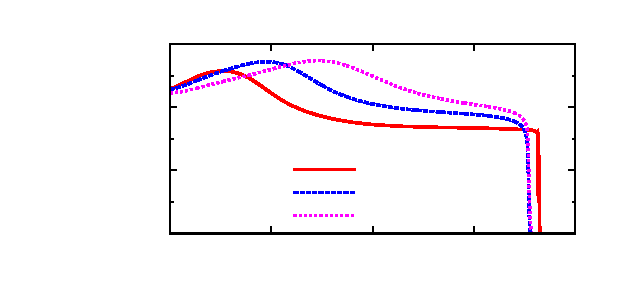
\includegraphics{1D_V_RO2}}%
    \gplfronttext
  \end{picture}%
\endgroup

  % GNUPLOT: LaTeX picture with Postscript
\begingroup
  \makeatletter
  \providecommand\color[2][]{%
    \GenericError{(gnuplot) \space\space\space\@spaces}{%
      Package color not loaded in conjunction with
      terminal option `colourtext'%
    }{See the gnuplot documentation for explanation.%
    }{Either use 'blacktext' in gnuplot or load the package
      color.sty in LaTeX.}%
    \renewcommand\color[2][]{}%
  }%
  \providecommand\includegraphics[2][]{%
    \GenericError{(gnuplot) \space\space\space\@spaces}{%
      Package graphicx or graphics not loaded%
    }{See the gnuplot documentation for explanation.%
    }{The gnuplot epslatex terminal needs graphicx.sty or graphics.sty.}%
    \renewcommand\includegraphics[2][]{}%
  }%
  \providecommand\rotatebox[2]{#2}%
  \@ifundefined{ifGPcolor}{%
    \newif\ifGPcolor
    \GPcolortrue
  }{}%
  \@ifundefined{ifGPblacktext}{%
    \newif\ifGPblacktext
    \GPblacktexttrue
  }{}%
  % define a \g@addto@macro without @ in the name:
  \let\gplgaddtomacro\g@addto@macro
  % define empty templates for all commands taking text:
  \gdef\gplbacktext{}%
  \gdef\gplfronttext{}%
  \makeatother
  \ifGPblacktext
    % no textcolor at all
    \def\colorrgb#1{}%
    \def\colorgray#1{}%
  \else
    % gray or color?
    \ifGPcolor
      \def\colorrgb#1{\color[rgb]{#1}}%
      \def\colorgray#1{\color[gray]{#1}}%
      \expandafter\def\csname LTw\endcsname{\color{white}}%
      \expandafter\def\csname LTb\endcsname{\color{black}}%
      \expandafter\def\csname LTa\endcsname{\color{black}}%
      \expandafter\def\csname LT0\endcsname{\color[rgb]{1,0,0}}%
      \expandafter\def\csname LT1\endcsname{\color[rgb]{0,1,0}}%
      \expandafter\def\csname LT2\endcsname{\color[rgb]{0,0,1}}%
      \expandafter\def\csname LT3\endcsname{\color[rgb]{1,0,1}}%
      \expandafter\def\csname LT4\endcsname{\color[rgb]{0,1,1}}%
      \expandafter\def\csname LT5\endcsname{\color[rgb]{1,1,0}}%
      \expandafter\def\csname LT6\endcsname{\color[rgb]{0,0,0}}%
      \expandafter\def\csname LT7\endcsname{\color[rgb]{1,0.3,0}}%
      \expandafter\def\csname LT8\endcsname{\color[rgb]{0.5,0.5,0.5}}%
    \else
      % gray
      \def\colorrgb#1{\color{black}}%
      \def\colorgray#1{\color[gray]{#1}}%
      \expandafter\def\csname LTw\endcsname{\color{white}}%
      \expandafter\def\csname LTb\endcsname{\color{black}}%
      \expandafter\def\csname LTa\endcsname{\color{black}}%
      \expandafter\def\csname LT0\endcsname{\color{black}}%
      \expandafter\def\csname LT1\endcsname{\color{black}}%
      \expandafter\def\csname LT2\endcsname{\color{black}}%
      \expandafter\def\csname LT3\endcsname{\color{black}}%
      \expandafter\def\csname LT4\endcsname{\color{black}}%
      \expandafter\def\csname LT5\endcsname{\color{black}}%
      \expandafter\def\csname LT6\endcsname{\color{black}}%
      \expandafter\def\csname LT7\endcsname{\color{black}}%
      \expandafter\def\csname LT8\endcsname{\color{black}}%
    \fi
  \fi
  \setlength{\unitlength}{0.0500bp}%
  \begin{picture}(5760.00,2520.00)%
    \gplgaddtomacro\gplbacktext{%
      \csname LTb\endcsname%
      \put(1342,704){\makebox(0,0)[r]{\strut{}1.0e-07}}%
      \put(1342,1221){\makebox(0,0)[r]{\strut{}1.0e-05}}%
      \put(1342,1739){\makebox(0,0)[r]{\strut{}1.0e-03}}%
      \put(1342,2256){\makebox(0,0)[r]{\strut{}1.0e-01}}%
      \put(1474,484){\makebox(0,0){\strut{} 0}}%
      \put(2446,484){\makebox(0,0){\strut{} 0.3}}%
      \put(3419,484){\makebox(0,0){\strut{} 0.6}}%
      \put(4391,484){\makebox(0,0){\strut{} 0.9}}%
      \put(5363,484){\makebox(0,0){\strut{} 1.2}}%
      \put(176,1480){\rotatebox{-270}{\makebox(0,0){\strut{}\vspace{-28pt}H$_2$O$_2$ Mass Fraction}}}%
      \put(3418,154){\makebox(0,0){\strut{}Time [ms]}}%
    }%
    \gplgaddtomacro\gplfronttext{%
      \csname LTb\endcsname%
      \put(2530,1317){\makebox(0,0)[r]{\strut{}$Z_{\rm st}$}}%
      \csname LTb\endcsname%
      \put(2530,1097){\makebox(0,0)[r]{\strut{}$Z = 0.2$}}%
      \csname LTb\endcsname%
      \put(2530,877){\makebox(0,0)[r]{\strut{}$Z = 0.3$}}%
    }%
    \gplbacktext
    \put(0,0){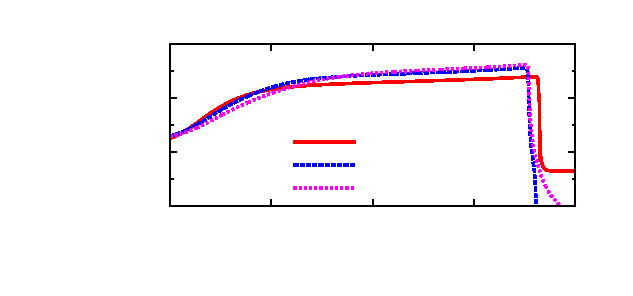
\includegraphics{1D_V_H2O2}}%
    \gplfronttext
  \end{picture}%
\endgroup

  \normalsize
  \caption{LFA profiles along $Z_{\rm st}$, $Z = 0.2$, and $Z = 0.3$ of the $8.0$ m/s case.}
  \label{fig:1D_V}
\end{figure}

The multibrachial structure of the inhomogeneous autoignition front is due to the variation in ignition delay time at different mixture fractions.  As shown in Fig.~\ref{fig:HRR_V}, the stabilization point is determined based on the threshold value of heat release rate.  Therefore, the ignition delay time of inhomogeneous autoignition can be determined accordingly, which corresponds to the heat release rate peak that exceeds $10^{12}$ J/m$^3$-s.  For the $8.0$ m/s case shown in Fig.~\ref{fig:tau}, the mixture is autoignited first at $Z = 0.24$, which corresponds to the stabilization point in Fig.~\ref{fig:HRR_V}.  Although the first stage ignition delay time, defined by the first heat release peak through low-temperature chemistry, increases monotonically as mixture fraction increases (temperature decreases), the overall ignition delay time reaches the shortest at $Z = 0.24$ due to the compensation of larger heat release after the first ignition stage~\cite{law12}, as shown in Fig.~\ref{fig:1D_V}.  As a consequence, although low-temperature chemistry is not the dominant chemical pathway at the stabilization point for the \emph{kinetically} stabilized case, it still influences the location of the stabilization point through the mixture fraction dependent heat and radical accumulation upstream.   

\begin{figure}
  \centering
  \scriptsize
  \resizebox{0.6\textwidth}{!}{% GNUPLOT: LaTeX picture with Postscript
\begingroup
  \makeatletter
  \providecommand\color[2][]{%
    \GenericError{(gnuplot) \space\space\space\@spaces}{%
      Package color not loaded in conjunction with
      terminal option `colourtext'%
    }{See the gnuplot documentation for explanation.%
    }{Either use 'blacktext' in gnuplot or load the package
      color.sty in LaTeX.}%
    \renewcommand\color[2][]{}%
  }%
  \providecommand\includegraphics[2][]{%
    \GenericError{(gnuplot) \space\space\space\@spaces}{%
      Package graphicx or graphics not loaded%
    }{See the gnuplot documentation for explanation.%
    }{The gnuplot epslatex terminal needs graphicx.sty or graphics.sty.}%
    \renewcommand\includegraphics[2][]{}%
  }%
  \providecommand\rotatebox[2]{#2}%
  \@ifundefined{ifGPcolor}{%
    \newif\ifGPcolor
    \GPcolortrue
  }{}%
  \@ifundefined{ifGPblacktext}{%
    \newif\ifGPblacktext
    \GPblacktexttrue
  }{}%
  % define a \g@addto@macro without @ in the name:
  \let\gplgaddtomacro\g@addto@macro
  % define empty templates for all commands taking text:
  \gdef\gplbacktext{}%
  \gdef\gplfronttext{}%
  \makeatother
  \ifGPblacktext
    % no textcolor at all
    \def\colorrgb#1{}%
    \def\colorgray#1{}%
  \else
    % gray or color?
    \ifGPcolor
      \def\colorrgb#1{\color[rgb]{#1}}%
      \def\colorgray#1{\color[gray]{#1}}%
      \expandafter\def\csname LTw\endcsname{\color{white}}%
      \expandafter\def\csname LTb\endcsname{\color{black}}%
      \expandafter\def\csname LTa\endcsname{\color{black}}%
      \expandafter\def\csname LT0\endcsname{\color[rgb]{1,0,0}}%
      \expandafter\def\csname LT1\endcsname{\color[rgb]{0,1,0}}%
      \expandafter\def\csname LT2\endcsname{\color[rgb]{0,0,1}}%
      \expandafter\def\csname LT3\endcsname{\color[rgb]{1,0,1}}%
      \expandafter\def\csname LT4\endcsname{\color[rgb]{0,1,1}}%
      \expandafter\def\csname LT5\endcsname{\color[rgb]{1,1,0}}%
      \expandafter\def\csname LT6\endcsname{\color[rgb]{0,0,0}}%
      \expandafter\def\csname LT7\endcsname{\color[rgb]{1,0.3,0}}%
      \expandafter\def\csname LT8\endcsname{\color[rgb]{0.5,0.5,0.5}}%
    \else
      % gray
      \def\colorrgb#1{\color{black}}%
      \def\colorgray#1{\color[gray]{#1}}%
      \expandafter\def\csname LTw\endcsname{\color{white}}%
      \expandafter\def\csname LTb\endcsname{\color{black}}%
      \expandafter\def\csname LTa\endcsname{\color{black}}%
      \expandafter\def\csname LT0\endcsname{\color{black}}%
      \expandafter\def\csname LT1\endcsname{\color{black}}%
      \expandafter\def\csname LT2\endcsname{\color{black}}%
      \expandafter\def\csname LT3\endcsname{\color{black}}%
      \expandafter\def\csname LT4\endcsname{\color{black}}%
      \expandafter\def\csname LT5\endcsname{\color{black}}%
      \expandafter\def\csname LT6\endcsname{\color{black}}%
      \expandafter\def\csname LT7\endcsname{\color{black}}%
      \expandafter\def\csname LT8\endcsname{\color{black}}%
    \fi
  \fi
  \setlength{\unitlength}{0.0500bp}%
  \begin{picture}(3600.00,2520.00)%
    \gplgaddtomacro\gplbacktext{%
      \csname LTb\endcsname%
      \put(1078,704){\makebox(0,0)[r]{\strut{} 1.05}}%
      \put(1078,1221){\makebox(0,0)[r]{\strut{} 1.07}}%
      \put(1078,1739){\makebox(0,0)[r]{\strut{} 1.09}}%
      \put(1078,2256){\makebox(0,0)[r]{\strut{} 1.11}}%
      \put(1210,484){\makebox(0,0){\strut{} 0}}%
      \put(1708,484){\makebox(0,0){\strut{} 0.1}}%
      \put(2207,484){\makebox(0,0){\strut{} 0.2}}%
      \put(2705,484){\makebox(0,0){\strut{} 0.3}}%
      \put(3203,484){\makebox(0,0){\strut{} 0.4}}%
      \put(176,1480){\rotatebox{-270}{\makebox(0,0){\strut{}\vspace{-28pt}Iginition Delay [ms]}}}%
      \put(2206,154){\makebox(0,0){\strut{}Z}}%
    }%
    \gplgaddtomacro\gplfronttext{%
    }%
    \gplbacktext
    \put(0,0){
\includegraphics{tau_t}}%
    \gplfronttext
  \end{picture}%
\endgroup
}
  \resizebox{0.6\textwidth}{!}{% GNUPLOT: LaTeX picture with Postscript
\begingroup
  \makeatletter
  \providecommand\color[2][]{%
    \GenericError{(gnuplot) \space\space\space\@spaces}{%
      Package color not loaded in conjunction with
      terminal option `colourtext'%
    }{See the gnuplot documentation for explanation.%
    }{Either use 'blacktext' in gnuplot or load the package
      color.sty in LaTeX.}%
    \renewcommand\color[2][]{}%
  }%
  \providecommand\includegraphics[2][]{%
    \GenericError{(gnuplot) \space\space\space\@spaces}{%
      Package graphicx or graphics not loaded%
    }{See the gnuplot documentation for explanation.%
    }{The gnuplot epslatex terminal needs graphicx.sty or graphics.sty.}%
    \renewcommand\includegraphics[2][]{}%
  }%
  \providecommand\rotatebox[2]{#2}%
  \@ifundefined{ifGPcolor}{%
    \newif\ifGPcolor
    \GPcolortrue
  }{}%
  \@ifundefined{ifGPblacktext}{%
    \newif\ifGPblacktext
    \GPblacktexttrue
  }{}%
  % define a \g@addto@macro without @ in the name:
  \let\gplgaddtomacro\g@addto@macro
  % define empty templates for all commands taking text:
  \gdef\gplbacktext{}%
  \gdef\gplfronttext{}%
  \makeatother
  \ifGPblacktext
    % no textcolor at all
    \def\colorrgb#1{}%
    \def\colorgray#1{}%
  \else
    % gray or color?
    \ifGPcolor
      \def\colorrgb#1{\color[rgb]{#1}}%
      \def\colorgray#1{\color[gray]{#1}}%
      \expandafter\def\csname LTw\endcsname{\color{white}}%
      \expandafter\def\csname LTb\endcsname{\color{black}}%
      \expandafter\def\csname LTa\endcsname{\color{black}}%
      \expandafter\def\csname LT0\endcsname{\color[rgb]{1,0,0}}%
      \expandafter\def\csname LT1\endcsname{\color[rgb]{0,1,0}}%
      \expandafter\def\csname LT2\endcsname{\color[rgb]{0,0,1}}%
      \expandafter\def\csname LT3\endcsname{\color[rgb]{1,0,1}}%
      \expandafter\def\csname LT4\endcsname{\color[rgb]{0,1,1}}%
      \expandafter\def\csname LT5\endcsname{\color[rgb]{1,1,0}}%
      \expandafter\def\csname LT6\endcsname{\color[rgb]{0,0,0}}%
      \expandafter\def\csname LT7\endcsname{\color[rgb]{1,0.3,0}}%
      \expandafter\def\csname LT8\endcsname{\color[rgb]{0.5,0.5,0.5}}%
    \else
      % gray
      \def\colorrgb#1{\color{black}}%
      \def\colorgray#1{\color[gray]{#1}}%
      \expandafter\def\csname LTw\endcsname{\color{white}}%
      \expandafter\def\csname LTb\endcsname{\color{black}}%
      \expandafter\def\csname LTa\endcsname{\color{black}}%
      \expandafter\def\csname LT0\endcsname{\color{black}}%
      \expandafter\def\csname LT1\endcsname{\color{black}}%
      \expandafter\def\csname LT2\endcsname{\color{black}}%
      \expandafter\def\csname LT3\endcsname{\color{black}}%
      \expandafter\def\csname LT4\endcsname{\color{black}}%
      \expandafter\def\csname LT5\endcsname{\color{black}}%
      \expandafter\def\csname LT6\endcsname{\color{black}}%
      \expandafter\def\csname LT7\endcsname{\color{black}}%
      \expandafter\def\csname LT8\endcsname{\color{black}}%
    \fi
  \fi
  \setlength{\unitlength}{0.0500bp}%
  \begin{picture}(3528.00,2520.00)%
    \gplgaddtomacro\gplbacktext{%
      \csname LTb\endcsname%
      \put(946,704){\makebox(0,0)[r]{\strut{} 0}}%
      \put(946,1221){\makebox(0,0)[r]{\strut{} 0.3}}%
      \put(946,1739){\makebox(0,0)[r]{\strut{} 0.6}}%
      \put(946,2256){\makebox(0,0)[r]{\strut{} 0.9}}%
      \put(1078,484){\makebox(0,0){\strut{} 0}}%
      \put(1591,484){\makebox(0,0){\strut{} 0.1}}%
      \put(2105,484){\makebox(0,0){\strut{} 0.2}}%
      \put(2618,484){\makebox(0,0){\strut{} 0.3}}%
      \put(3131,484){\makebox(0,0){\strut{} 0.4}}%
      \put(176,1480){\rotatebox{-270}{\makebox(0,0){\strut{}\vspace{-28pt}First Stage Ignition Delay [ms]}}}%
      \put(2104,154){\makebox(0,0){\strut{}Z}}%
    }%
    \gplgaddtomacro\gplfronttext{%
    }%
    \gplbacktext
    \put(0,0){
\includegraphics{ch-dynamics/tau_1}}%
    \gplfronttext
  \end{picture}%
\endgroup
}
  \normalsize
  \caption{LFA results on the mixture fraction dependent total and first stage ignition delay times of the $8.0$ m/s case.}
  \label{fig:tau}
\end{figure}          

However, although the cases discussed are all initiated by inhomogeneous autoignition, the stabilization of the final structure depends on the dominant transport processes, which are influenced by the inlet velocities.  At $8.0$ m/s, heat and radical back diffusion from the autoignition front to upstream is not able to keep up with convection; therefore, the reacting front is \emph{kinetically} stabilized.  At $3.2$ m/s, as flow convection is weaker, diffusion processes become inherently important and couple with chemical reactions to induce a flame front propagating upstream.  However, the propagation speed of the flame varies with composition and temperature.  As a consequence, around $Z_{\rm st}$, where higher temperature and near-stoichiometric mixture composition enable higher local flame speed, the propagation of the reacting front balances the incoming flow velocity.  However, such a balance fails at richer mixture fractions where \emph{kinetic} stabilization dominates due to enhanced NTC-affected autoignition at richer mixture fractions as demonstrated in Fig.~\ref{fig:tau}.  At $2.4$ m/s, back diffusion is important at all mixture fractions such that the reacting front propagates upstream at the local flame speed, as determined by the local composition and temperature.  Due to the increased temperature and species stratification and the reduced thermal and radical accumulation from autoignition, the propagation speed of this reacting front is less influenced by inhomogeneous autoignition, as demonstrated with CEMA and LFA.  The structure of this \emph{kinematically} stabilized reacting front, which is generally tribrachial, is therefore determined by the variation of the local flame speed. 

\subsection{Stabilization Regime Diagram}

The above sections have demonstrated the transport effects on the thermal and chemical structure of the lifted coflow flames as well as the stabilization mechanisms.  Combining these results with the chemical effects demonstrated by changing the coflow boundary temperature in Sec.~\ref{sec:dynamics-T}, a two-dimensional stabilization regime diagram is proposed, as shown in Fig.~\ref{fig:2D-regime}.  

\begin{figure}
  \centering
  \scriptsize
  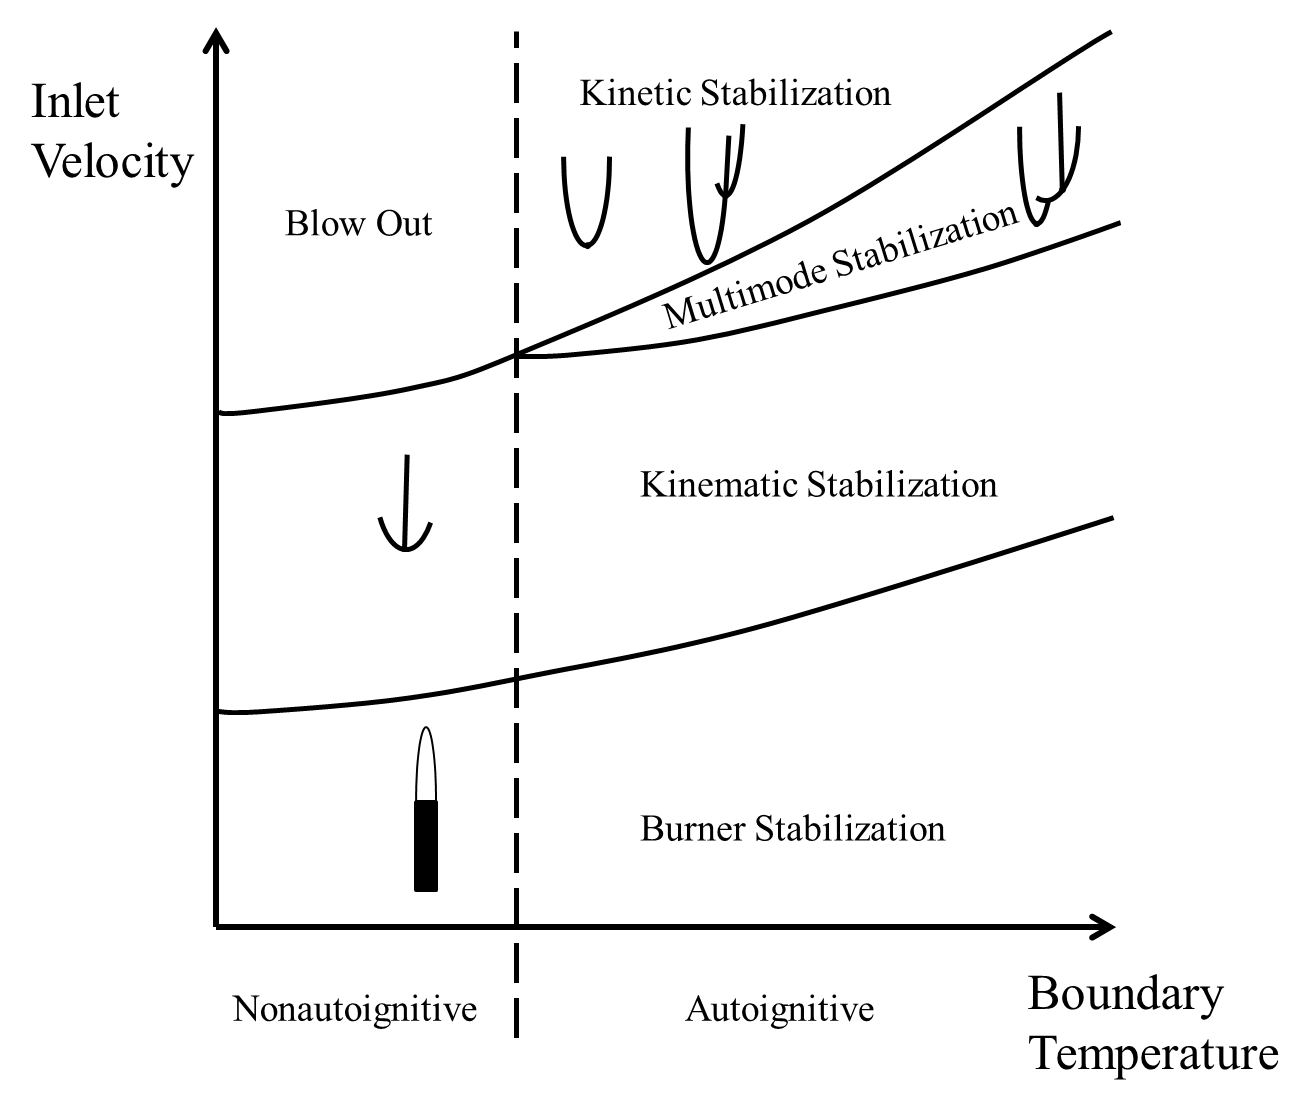
\includegraphics[width=0.8\textwidth]{ch-dynamics/2D-regime.png}
  \normalsize
  \caption{A qualitative regime diagram for the stabilization mechanisms as the boundary temperature and inlet velocity vary. }
  \label{fig:2D-regime}
\end{figure}

Qualitatively, when the boundary temperature is not high enough to activate autoignition, the lifted flame appears as the classical triple flame and is \emph{kinematically} stabilized.  When the inlet velocity is below or above certain threshold values, the triple flame becomes attached to the burner or is blown out, respectively.  

As the boundary temperature is elevated enough to activate autoignition, increasing the inlet velocity while keeping constant boundary temperature, the flame stabilization mechanism transits from burner stabilization to a \emph{kinematic} balance between flame speed and incoming flow velocity, then to multimode stabilization influenced by both flame propagation and inhomogeneous autoignition, and finally to \emph {kinetic} stabilization governed by inhomogeneous autoignition.  It is expected that the crossover velocities between regimes increase with increasing boundary temperature because flame speed generally increases at higher temperature.  However, it is difficult to quantify these boundaries as local composition and temperature vary in the streamwise direction, and, therefore, the reference flame speed cannot be calculated based on the upstream boundary conditions.  Furthermore, local flame front curvature, cross-stream species stratification, and flow divergence approaching the flame front also modify the flame speed.  As a consequence, only a qualitative trend is demonstrated in Fig.~\ref{fig:2D-regime}.  

Similarly, if the boundary temperature increases at fixed inlet velocity, transition from blow out to burner stabilized regimes is achieved by moving horizontally across the regime diagram, which was discussed in Sec.~\ref{sec:dynamics-T}.     

%---------------------------------------------

\section{Flame Dynamics in Oscillating Flows}

In this section, unsteady nonpremixed DME/air coflow flames under autoignitive conditions are computationally studied to elucidate the coupling between unsteady fluid dynamics and chemical kinetics.  Various oscillation frequencies were imposed on the inlet velocity, with the maximum and minimum velocities maintained the same as those in Sec.~\ref{sec:dynamics-V}, which correspond to an autoignition front and a tribrachial flame, respectively.  Low frequency oscillation ranging from 25 to 100 Hz, which covers buoyancy-driven instability frequencies~\cite{mohammed98,dworkin07} and acoustic-driven oscillation frequencies in gas turbines~\cite{temme12} is considered.  As the steady cases correspond to different combustion modes, it is expected that, at certain frequencies of velocity oscillation, the dominant combustion process will shift between the nonpremixed tribrachial flame mode and the autoignition mode.  Therefore, the transition in combustion mode is first presented.  The thermal and chemical differences during such transition and the transition mechanism are then discussed.  Finally, the effects of oscillation frequency on the coupling of fluid dynamics and chemical kinetics is elucidated.  The understanding of the coupling effects of chemistry and transport obtained lays the foundation for future turbulent studies.

\subsection{Thermal Structure}

As the largest and smallest inlet velocity cases were designed to match the two extreme cases in Sec.~\ref{sec:dynamics-V}, which are of different thermal structures, it is expected that similar thermal structures will be obtained.  Furthermore, these thermal structures might transition back and forth in response to the oscillating flow field.  Indeed, such transitions were observed for all three frequencies.  For example, the evolution of the thermal structure of the $100$ Hz case, in terms of the heat release rate profile, is demonstrated in Fig.~\ref{fig:HRR_100Hz}.  The oscillation cycle starts with the largest inlet velocity of $8.0$ m/s, and the minimum inlet velocity ($2.4$ m/s) is achieved at half cycle.  

\begin{figure}[t]
  \centering
  \scriptsize
  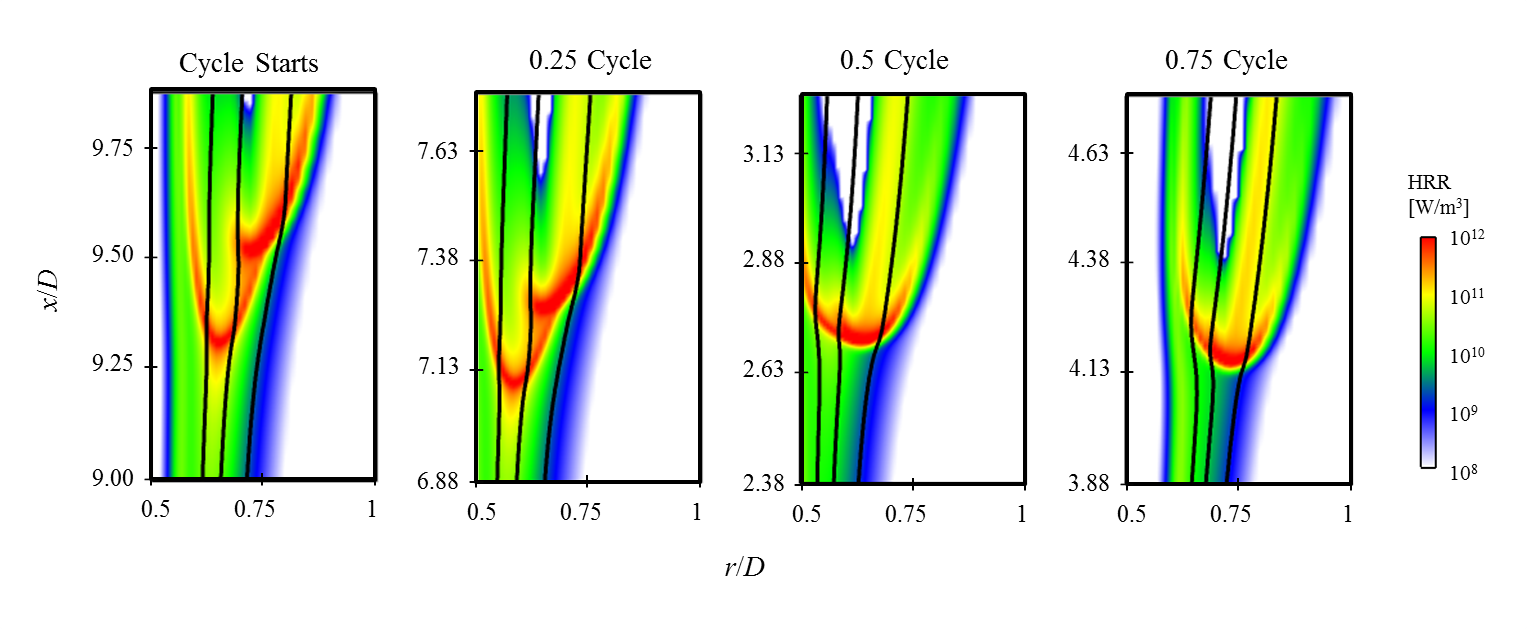
\includegraphics[trim=6.5mm 7.5mm 7mm 8mm, clip=true, width=1.0\textwidth]{ch-dynamics/HRR_100Hz.png}
  \normalsize
  \caption{Heat release rate [W/m$^3$] profile evolution during one oscillation cycle at $100$ Hz.  The iso-contours of $Z_{\rm st} = 0.1$, $Z = 0.2$, and $Z = 0.3$ are outlined from right to left in solid lines, respectively.}
  \label{fig:HRR_100Hz}
\end{figure}

At $8.0$ m/s, the multibrachial thermal structure is located furthest downstream.  The leading point, which is defined as the most upstream point that has the heat release rate value of $10^{12}$ W/m$^3$, is located at mixture fraction $Z = 0.24$.  As the inlet velocity decreases, the multibrachial structure moves upstream, without obvious change of the leading point location, in terms of mixture fraction.  When the inlet velocity reaches its minimum, the multibrachial structure transitions to a tribrachial structure, and the leading point switches to $Z = 0.14$.  As the flow velocity increases, the tribrachial structure is pushed downstream, and both its tribrachial shape and its leading point mixture fraction remain unchanged.  The thermal structure returns to that of multibrachial when the flow velocity further increases.  Such transitions in structure repeat once a new oscillation cycle starts.

\subsection{Differentiation of Combustion Mode}

In Sec.~\ref{sec:dynamics-V} the morphology of the thermal structures are related to two different combustion modes: tribrachial flame and autoignition.  Specifically, at steady state, the multibrachial structure in the $8.0$ m/s case is an autoignition front, while the $2.4$ m/s case is a tribrachial flame.  In the previouly presented steady cases, species mass fraction profiles at the inlet of the two-dimensional computation are treated as the initial conditions for one-dimensional Lagrangian Flamelet Analysis~\cite{pitsch98a}, which only considers diffusion processes parallel to the mixture fraction gradient and neglects those in the normal direction.  When the LFA prediction agrees with the CFD result, transport in the normal direction of the mixture fraction gradient is negligible, and autoignition is the dominant combustion process.  However, due to the unsteadiness in the oscillating cases, such comparison between LFA and CFD is no longer applicable, and a new criterion to differentiate the modes of tribrachial flame and autoignition needs to be identified and validated against the steady cases.

A density-weighted displacement speed, $S_d$, is often used to distinguish between deflagrations and spontaneous ignition fronts in HCCI combustion~\cite{yoo13}, which is defined from an iso-line of species $k$ as~\cite{ruetsch95,im99}:

\begin{equation} \label{eq:sd}
S_d = \frac{1}{\rho{_u} |\nabla Y_k|} \left(\dot{\omega}{_k} - \pp{\rho Y_k V_{j,k}}{x_j} \right),
\end{equation}
where $Y_k$, $V_{j,k}$, and $\dot{\omega}{_k}$ denote species mass fraction, diffusion velocity in the $j$-direction, and net production rate, respectively, and $\rho {_u}$ is the density of the unburnt mixture.  The choice of species $k$ and its iso-line value can be ambiguous.  Therefore, major products, such as CO$_2$, H$_2$O, H$_2$, CO, and combinations of these products have been tested, and the sampling location is chosen as the leading point, as defined above, to enable further comparison with the steady cases.  $S_d$ at the leading point is insensitive to the choice of species, for less than $5$\% difference was observed across all the combinations.  Consequently, H$_2$O was chosen for simplicity.  Both the laminar flame speed $S_L$ and the unburnt mixture density $\rho {_u}$ were obtained from laminar flame speed calculations using the FlameMaster code~\cite{flamemaster}.  The composition and temperature boundary conditions for the laminar flame speed calculations were based on the sampled mixture fraction at the leading point and linearly interpolated, in the mixture fraction space, between the corresponding inlet values of the fuel and coflow streams.  

Following the above procedure, displacement velocities were calculated for all three oscillation frequency cases, with $20$ points per cycle, to demonstrate their evolution.  Furthermore, as shown in Fig.~\ref{fig:sd_evo}, $S_d/S_L$ for the two steady cases ($2.4$ and $8.0$ m/s) were similarly calculated to validate this definition of normalized displacement velocity and differentiate between tribrachial flame and autoignition.  For clarity, only the 100 Hz case is included in Fig.~\ref{fig:sd_evo} to elucidate its evolution, and the effect of the oscillation frequency will be discussed in Sec.\ref{sec:frq}.

\begin{figure}[t]
  \centering
  \scriptsize
  \resizebox{1.0\textwidth}{!}{% GNUPLOT: LaTeX picture with Postscript
\begingroup
  \makeatletter
  \providecommand\color[2][]{%
    \GenericError{(gnuplot) \space\space\space\@spaces}{%
      Package color not loaded in conjunction with
      terminal option `colourtext'%
    }{See the gnuplot documentation for explanation.%
    }{Either use 'blacktext' in gnuplot or load the package
      color.sty in LaTeX.}%
    \renewcommand\color[2][]{}%
  }%
  \providecommand\includegraphics[2][]{%
    \GenericError{(gnuplot) \space\space\space\@spaces}{%
      Package graphicx or graphics not loaded%
    }{See the gnuplot documentation for explanation.%
    }{The gnuplot epslatex terminal needs graphicx.sty or graphics.sty.}%
    \renewcommand\includegraphics[2][]{}%
  }%
  \providecommand\rotatebox[2]{#2}%
  \@ifundefined{ifGPcolor}{%
    \newif\ifGPcolor
    \GPcolortrue
  }{}%
  \@ifundefined{ifGPblacktext}{%
    \newif\ifGPblacktext
    \GPblacktexttrue
  }{}%
  % define a \g@addto@macro without @ in the name:
  \let\gplgaddtomacro\g@addto@macro
  % define empty templates for all commands taking text:
  \gdef\gplbacktext{}%
  \gdef\gplfronttext{}%
  \makeatother
  \ifGPblacktext
    % no textcolor at all
    \def\colorrgb#1{}%
    \def\colorgray#1{}%
  \else
    % gray or color?
    \ifGPcolor
      \def\colorrgb#1{\color[rgb]{#1}}%
      \def\colorgray#1{\color[gray]{#1}}%
      \expandafter\def\csname LTw\endcsname{\color{white}}%
      \expandafter\def\csname LTb\endcsname{\color{black}}%
      \expandafter\def\csname LTa\endcsname{\color{black}}%
      \expandafter\def\csname LT0\endcsname{\color[rgb]{1,0,0}}%
      \expandafter\def\csname LT1\endcsname{\color[rgb]{0,1,0}}%
      \expandafter\def\csname LT2\endcsname{\color[rgb]{0,0,1}}%
      \expandafter\def\csname LT3\endcsname{\color[rgb]{1,0,1}}%
      \expandafter\def\csname LT4\endcsname{\color[rgb]{0,1,1}}%
      \expandafter\def\csname LT5\endcsname{\color[rgb]{1,1,0}}%
      \expandafter\def\csname LT6\endcsname{\color[rgb]{0,0,0}}%
      \expandafter\def\csname LT7\endcsname{\color[rgb]{1,0.3,0}}%
      \expandafter\def\csname LT8\endcsname{\color[rgb]{0.5,0.5,0.5}}%
    \else
      % gray
      \def\colorrgb#1{\color{black}}%
      \def\colorgray#1{\color[gray]{#1}}%
      \expandafter\def\csname LTw\endcsname{\color{white}}%
      \expandafter\def\csname LTb\endcsname{\color{black}}%
      \expandafter\def\csname LTa\endcsname{\color{black}}%
      \expandafter\def\csname LT0\endcsname{\color{black}}%
      \expandafter\def\csname LT1\endcsname{\color{black}}%
      \expandafter\def\csname LT2\endcsname{\color{black}}%
      \expandafter\def\csname LT3\endcsname{\color{black}}%
      \expandafter\def\csname LT4\endcsname{\color{black}}%
      \expandafter\def\csname LT5\endcsname{\color{black}}%
      \expandafter\def\csname LT6\endcsname{\color{black}}%
      \expandafter\def\csname LT7\endcsname{\color{black}}%
      \expandafter\def\csname LT8\endcsname{\color{black}}%
    \fi
  \fi
  \setlength{\unitlength}{0.0500bp}%
  \begin{picture}(5760.00,4032.00)%
    \gplgaddtomacro\gplbacktext{%
      \csname LTb\endcsname%
      \put(588,704){\makebox(0,0)[r]{\strut{} 0}}%
      \put(588,1317){\makebox(0,0)[r]{\strut{} 2}}%
      \put(588,1929){\makebox(0,0)[r]{\strut{} 4}}%
      \put(588,2542){\makebox(0,0)[r]{\strut{} 6}}%
      \put(588,3154){\makebox(0,0)[r]{\strut{} 8}}%
      \put(588,3767){\makebox(0,0)[r]{\strut{} 10}}%
      \put(720,484){\makebox(0,0){\strut{} 0}}%
      \put(1260,484){\makebox(0,0){\strut{} 0.25}}%
      \put(1800,484){\makebox(0,0){\strut{} 0.5}}%
      \put(2340,484){\makebox(0,0){\strut{} 0.75}}%
      \put(2880,484){\makebox(0,0){\strut{} 1}}%
      \put(3419,484){\makebox(0,0){\strut{} 1.25}}%
      \put(3959,484){\makebox(0,0){\strut{} 1.5}}%
      \put(4499,484){\makebox(0,0){\strut{} 1.75}}%
      \put(5039,484){\makebox(0,0){\strut{} 2}}%
      \put(5171,704){\makebox(0,0)[l]{\strut{} 0}}%
      \put(5171,1317){\makebox(0,0)[l]{\strut{} 3}}%
      \put(5171,1929){\makebox(0,0)[l]{\strut{} 6}}%
      \put(5171,2542){\makebox(0,0)[l]{\strut{} 9}}%
      \put(5171,3154){\makebox(0,0)[l]{\strut{} 12}}%
      \put(5171,3767){\makebox(0,0)[l]{\strut{} 15}}%
      \put(-50,2235){\rotatebox{-270}{\makebox(0,0){\strut{}\vspace{-28pt}$S_d/S_L$}}}%
      \put(5808,2235){\rotatebox{-270}{\makebox(0,0){\strut{}\vspace{28pt}$x_d/D$}}}%
      \put(2879,154){\makebox(0,0){\strut{}Cycle}}%
    }%
    \gplgaddtomacro\gplfronttext{%
      \csname LTb\endcsname%
      \put(2068,3679){\makebox(0,0)[r]{\strut{}Steady $S_d/S_L$}}%
      \csname LTb\endcsname%
      \put(2068,3503){\makebox(0,0)[r]{\strut{}$S_d/S_L$}}%
      \csname LTb\endcsname%
      \put(2068,3327){\makebox(0,0)[r]{\strut{}$x_d/D$}}%
    }%
    \gplbacktext
    \put(0,0){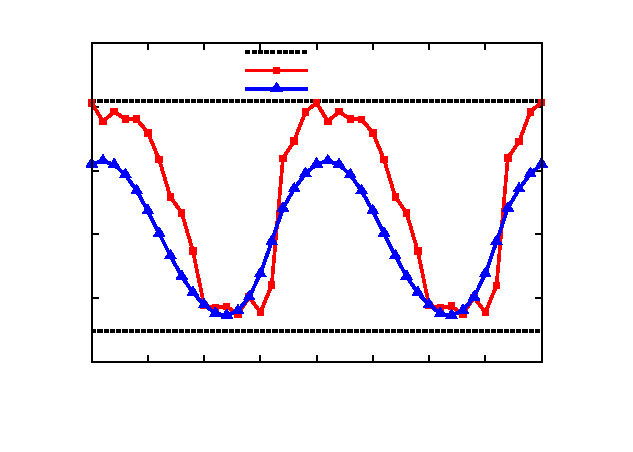
\includegraphics{sd_evo}}%
    \gplfronttext
  \end{picture}%
\endgroup
}
  \normalsize
  \caption{Normalized displacement velocity (red) and leading point location (blue) time history profiles at $100$ Hz.}
  \label{fig:sd_evo}
\end{figure}

The normalized displacement velocities for the steady autoignition front and tribrachial flame are shown in Fig.~\ref{fig:sd_evo} as the top and bottom horizontal lines, respectively.  The $S_d/S_L$ for the steady tribrachial flame is around unity, while this value is around eight for the autoignition front.  These values are similar to those in HCCI combustion studies~\cite{yoo13} and therefore can be used to benchmark the unsteady cases.  The periodic time history profile of $S_d/S_L$ is bounded by but does not fully reach the two steady values, indicating that, while the chemical structure responds to the flow dynamics, such response is not fast enough to reach steady-state.  

When $S_d/S_L$ approaches the tribrachial flame limit, its value is almost constant, while the change near the autoignition limit is more sinusoidal.  Moreover, $S_d/S_L$ changes more abruptly when the combustion mode switches from tribrachial flame to autoignition.  Compared to the profile of the normalized leading point location ($x_d/D$), which is almost sinusoidal, the profile of the normalized displacement velocity is asymmetric, indicating that the transition from tribrachial flame to autoignition as the inlet velocity increases is not an exact reverse process of the transition from autoignition to tribrachial flame.  Indeed, as shown in Fig.~\ref{fig:HRR_100Hz}, although the inlet velocities at $0.25$ and $0.75$ cycle are the same, the structures demonstrate different morphologies during the cycle of decreasing- and increasing-velocity: there is hysteresis during the transition.

Such hysteresis is demonstrated more clearly in Fig.~\ref{fig:sd_hys}, where $S_d/S_L$ is plotted against the inlet velocity.  Given the same inlet velocity, the reacting fronts have different displacement velocities during the cycle of decreasing- and increasing-velocity.  Additional evidence of hysteresis, shown in Fig.~\ref{fig:HRR_100Hz}, is the shift in the location of the leading point in the mixture fraction space: $Z = 0.14$ when the tribrachial flame dominates and $Z = 0.24$ when autoignition dominates.  The shift in the leading point mixture fraction as well as the displacement velocity indicates different dominant chemical reactions, and analysis of the dominant chemical reactions will reveal the mechanism of the hysteresis.

\begin{figure}[t]
  \centering
  \scriptsize
  \resizebox{1.0\textwidth}{!}{% GNUPLOT: LaTeX picture with Postscript
\begingroup
  \makeatletter
  \providecommand\color[2][]{%
    \GenericError{(gnuplot) \space\space\space\@spaces}{%
      Package color not loaded in conjunction with
      terminal option `colourtext'%
    }{See the gnuplot documentation for explanation.%
    }{Either use 'blacktext' in gnuplot or load the package
      color.sty in LaTeX.}%
    \renewcommand\color[2][]{}%
  }%
  \providecommand\includegraphics[2][]{%
    \GenericError{(gnuplot) \space\space\space\@spaces}{%
      Package graphicx or graphics not loaded%
    }{See the gnuplot documentation for explanation.%
    }{The gnuplot epslatex terminal needs graphicx.sty or graphics.sty.}%
    \renewcommand\includegraphics[2][]{}%
  }%
  \providecommand\rotatebox[2]{#2}%
  \@ifundefined{ifGPcolor}{%
    \newif\ifGPcolor
    \GPcolortrue
  }{}%
  \@ifundefined{ifGPblacktext}{%
    \newif\ifGPblacktext
    \GPblacktexttrue
  }{}%
  % define a \g@addto@macro without @ in the name:
  \let\gplgaddtomacro\g@addto@macro
  % define empty templates for all commands taking text:
  \gdef\gplbacktext{}%
  \gdef\gplfronttext{}%
  \makeatother
  \ifGPblacktext
    % no textcolor at all
    \def\colorrgb#1{}%
    \def\colorgray#1{}%
  \else
    % gray or color?
    \ifGPcolor
      \def\colorrgb#1{\color[rgb]{#1}}%
      \def\colorgray#1{\color[gray]{#1}}%
      \expandafter\def\csname LTw\endcsname{\color{white}}%
      \expandafter\def\csname LTb\endcsname{\color{black}}%
      \expandafter\def\csname LTa\endcsname{\color{black}}%
      \expandafter\def\csname LT0\endcsname{\color[rgb]{1,0,0}}%
      \expandafter\def\csname LT1\endcsname{\color[rgb]{0,1,0}}%
      \expandafter\def\csname LT2\endcsname{\color[rgb]{0,0,1}}%
      \expandafter\def\csname LT3\endcsname{\color[rgb]{1,0,1}}%
      \expandafter\def\csname LT4\endcsname{\color[rgb]{0,1,1}}%
      \expandafter\def\csname LT5\endcsname{\color[rgb]{1,1,0}}%
      \expandafter\def\csname LT6\endcsname{\color[rgb]{0,0,0}}%
      \expandafter\def\csname LT7\endcsname{\color[rgb]{1,0.3,0}}%
      \expandafter\def\csname LT8\endcsname{\color[rgb]{0.5,0.5,0.5}}%
    \else
      % gray
      \def\colorrgb#1{\color{black}}%
      \def\colorgray#1{\color[gray]{#1}}%
      \expandafter\def\csname LTw\endcsname{\color{white}}%
      \expandafter\def\csname LTb\endcsname{\color{black}}%
      \expandafter\def\csname LTa\endcsname{\color{black}}%
      \expandafter\def\csname LT0\endcsname{\color{black}}%
      \expandafter\def\csname LT1\endcsname{\color{black}}%
      \expandafter\def\csname LT2\endcsname{\color{black}}%
      \expandafter\def\csname LT3\endcsname{\color{black}}%
      \expandafter\def\csname LT4\endcsname{\color{black}}%
      \expandafter\def\csname LT5\endcsname{\color{black}}%
      \expandafter\def\csname LT6\endcsname{\color{black}}%
      \expandafter\def\csname LT7\endcsname{\color{black}}%
      \expandafter\def\csname LT8\endcsname{\color{black}}%
    \fi
  \fi
  \setlength{\unitlength}{0.0500bp}%
  \begin{picture}(5760.00,4032.00)%
    \gplgaddtomacro\gplbacktext{%
      \csname LTb\endcsname%
      \put(588,704){\makebox(0,0)[r]{\strut{} 0}}%
      \put(588,1317){\makebox(0,0)[r]{\strut{} 2}}%
      \put(588,1929){\makebox(0,0)[r]{\strut{} 4}}%
      \put(588,2542){\makebox(0,0)[r]{\strut{} 6}}%
      \put(588,3154){\makebox(0,0)[r]{\strut{} 8}}%
      \put(588,3767){\makebox(0,0)[r]{\strut{} 10}}%
      \put(720,484){\makebox(0,0){\strut{} 0}}%
      \put(1584,484){\makebox(0,0){\strut{} 2}}%
      \put(2448,484){\makebox(0,0){\strut{} 4}}%
      \put(3311,484){\makebox(0,0){\strut{} 6}}%
      \put(4175,484){\makebox(0,0){\strut{} 8}}%
      \put(5039,484){\makebox(0,0){\strut{} 10}}%
      \put(-50,2235){\rotatebox{-270}{\makebox(0,0){\strut{}\vspace{-28pt}$S_d/S_L$}}}%
      \put(2879,154){\makebox(0,0){\strut{}$U_{\rm inlet}$}}%
      \put(2232,1041){\makebox(0,0)[l]{\strut{}Induction period}}%
      \put(1066,2848){\makebox(0,0)[l]{\strut{}Decreasing-velocity}}%
      \put(3743,1470){\makebox(0,0)[l]{\strut{}Increasing-velocity}}%
    }%
    \gplgaddtomacro\gplfronttext{%
      \csname LTb\endcsname%
      \put(1377,3618){\makebox(0,0)[r]{\strut{}Steady}}%
      \csname LTb\endcsname%
      \put(1377,3442){\makebox(0,0)[r]{\strut{}100 Hz}}%
    }%
    \gplbacktext
    \put(0,0){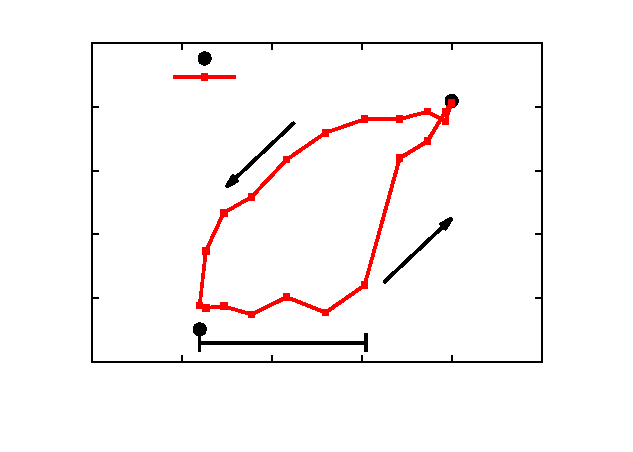
\includegraphics{sd_hys_100Hz}}%
    \gplfronttext
  \end{picture}%
\endgroup
}
  \normalsize
  \caption{Normalized displacement velocities at various inlet velocities for two steady cases and the 100 Hz oscillating unsteady cases.}
  \label{fig:sd_hys}
\end{figure}

From the steady case analysis in Sec.~\ref{sec:dynamics-V}, the dominant chemical pathways are found to be different at the leading point of the tribrachial flame and autoignition front.  Specifically, the hydrogen peroxide branching reaction (H$_2$O$_2$ + M $\Longleftrightarrow$ OH + OH + M) is the dominant chain branching reaction at the leading point of the autoignition front, while the H radical branching reaction (H + O$_2$ $\Longleftrightarrow$ O + OH) is the most important chain branching reaction at the tribrachial flame leading point.  Due to the longer residence time, hydrogen peroxide accumulation is much higher upstream of the autoignition front compared to the tribrachial flame front.

\begin{figure}[t]
  \centering
  \scriptsize
  \resizebox{0.49\textwidth}{!}{% GNUPLOT: LaTeX picture with Postscript
\begingroup
  \makeatletter
  \providecommand\color[2][]{%
    \GenericError{(gnuplot) \space\space\space\@spaces}{%
      Package color not loaded in conjunction with
      terminal option `colourtext'%
    }{See the gnuplot documentation for explanation.%
    }{Either use 'blacktext' in gnuplot or load the package
      color.sty in LaTeX.}%
    \renewcommand\color[2][]{}%
  }%
  \providecommand\includegraphics[2][]{%
    \GenericError{(gnuplot) \space\space\space\@spaces}{%
      Package graphicx or graphics not loaded%
    }{See the gnuplot documentation for explanation.%
    }{The gnuplot epslatex terminal needs graphicx.sty or graphics.sty.}%
    \renewcommand\includegraphics[2][]{}%
  }%
  \providecommand\rotatebox[2]{#2}%
  \@ifundefined{ifGPcolor}{%
    \newif\ifGPcolor
    \GPcolortrue
  }{}%
  \@ifundefined{ifGPblacktext}{%
    \newif\ifGPblacktext
    \GPblacktexttrue
  }{}%
  % define a \g@addto@macro without @ in the name:
  \let\gplgaddtomacro\g@addto@macro
  % define empty templates for all commands taking text:
  \gdef\gplbacktext{}%
  \gdef\gplfronttext{}%
  \makeatother
  \ifGPblacktext
    % no textcolor at all
    \def\colorrgb#1{}%
    \def\colorgray#1{}%
  \else
    % gray or color?
    \ifGPcolor
      \def\colorrgb#1{\color[rgb]{#1}}%
      \def\colorgray#1{\color[gray]{#1}}%
      \expandafter\def\csname LTw\endcsname{\color{white}}%
      \expandafter\def\csname LTb\endcsname{\color{black}}%
      \expandafter\def\csname LTa\endcsname{\color{black}}%
      \expandafter\def\csname LT0\endcsname{\color[rgb]{1,0,0}}%
      \expandafter\def\csname LT1\endcsname{\color[rgb]{0,1,0}}%
      \expandafter\def\csname LT2\endcsname{\color[rgb]{0,0,1}}%
      \expandafter\def\csname LT3\endcsname{\color[rgb]{1,0,1}}%
      \expandafter\def\csname LT4\endcsname{\color[rgb]{0,1,1}}%
      \expandafter\def\csname LT5\endcsname{\color[rgb]{1,1,0}}%
      \expandafter\def\csname LT6\endcsname{\color[rgb]{0,0,0}}%
      \expandafter\def\csname LT7\endcsname{\color[rgb]{1,0.3,0}}%
      \expandafter\def\csname LT8\endcsname{\color[rgb]{0.5,0.5,0.5}}%
    \else
      % gray
      \def\colorrgb#1{\color{black}}%
      \def\colorgray#1{\color[gray]{#1}}%
      \expandafter\def\csname LTw\endcsname{\color{white}}%
      \expandafter\def\csname LTb\endcsname{\color{black}}%
      \expandafter\def\csname LTa\endcsname{\color{black}}%
      \expandafter\def\csname LT0\endcsname{\color{black}}%
      \expandafter\def\csname LT1\endcsname{\color{black}}%
      \expandafter\def\csname LT2\endcsname{\color{black}}%
      \expandafter\def\csname LT3\endcsname{\color{black}}%
      \expandafter\def\csname LT4\endcsname{\color{black}}%
      \expandafter\def\csname LT5\endcsname{\color{black}}%
      \expandafter\def\csname LT6\endcsname{\color{black}}%
      \expandafter\def\csname LT7\endcsname{\color{black}}%
      \expandafter\def\csname LT8\endcsname{\color{black}}%
    \fi
  \fi
  \setlength{\unitlength}{0.0500bp}%
  \begin{picture}(4320.00,3024.00)%
    \gplgaddtomacro\gplbacktext{%
      \csname LTb\endcsname%
      \put(948,704){\makebox(0,0)[r]{\strut{}0.0e+00}}%
      \put(948,1115){\makebox(0,0)[r]{\strut{}6.0e-03}}%
      \put(948,1526){\makebox(0,0)[r]{\strut{}1.2e-02}}%
      \put(948,1937){\makebox(0,0)[r]{\strut{}1.8e-02}}%
      \put(948,2348){\makebox(0,0)[r]{\strut{}2.4e-02}}%
      \put(948,2759){\makebox(0,0)[r]{\strut{}3.0e-02}}%
      \put(1080,484){\makebox(0,0){\strut{} 0}}%
      \put(1649,484){\makebox(0,0){\strut{} 2}}%
      \put(2217,484){\makebox(0,0){\strut{} 4}}%
      \put(2786,484){\makebox(0,0){\strut{} 6}}%
      \put(3354,484){\makebox(0,0){\strut{} 8}}%
      \put(3923,484){\makebox(0,0){\strut{} 10}}%
      \put(-218,1731){\rotatebox{-270}{\makebox(0,0){\strut{}\vspace{-28pt}$Y_{\rm H_2O_2}$}}}%
      \put(2501,154){\makebox(0,0){\strut{}$x/D$}}%
      \put(1506,2896){\makebox(0,0)[l]{\strut{}$Z = 0.14$ Decreasing-velocity Cycle}}%
    }%
    \gplgaddtomacro\gplfronttext{%
      \csname LTb\endcsname%
      \put(2763,1899){\makebox(0,0)[r]{\strut{}0.5 cycle}}%
      \csname LTb\endcsname%
      \put(2763,2075){\makebox(0,0)[r]{\strut{}0.45 cycle}}%
      \csname LTb\endcsname%
      \put(2763,2251){\makebox(0,0)[r]{\strut{}0.25 cycle}}%
      \csname LTb\endcsname%
      \put(2763,2427){\makebox(0,0)[r]{\strut{}Steady 8.0 m/s}}%
      \csname LTb\endcsname%
      \put(2763,2603){\makebox(0,0)[r]{\strut{}Steady 2.4 m/s}}%
    }%
    \gplbacktext
    \put(0,0){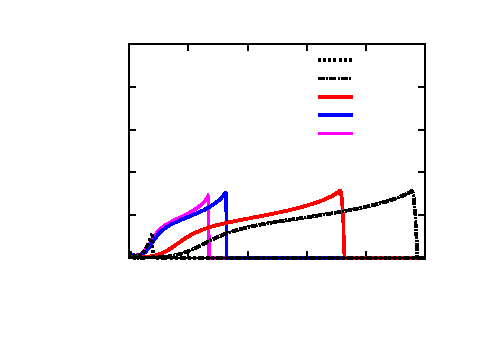
\includegraphics{H2O2_up_Z14}}%
    \gplfronttext
  \end{picture}%
\endgroup
}
  \resizebox{0.49\textwidth}{!}{% GNUPLOT: LaTeX picture with Postscript
\begingroup
  \makeatletter
  \providecommand\color[2][]{%
    \GenericError{(gnuplot) \space\space\space\@spaces}{%
      Package color not loaded in conjunction with
      terminal option `colourtext'%
    }{See the gnuplot documentation for explanation.%
    }{Either use 'blacktext' in gnuplot or load the package
      color.sty in LaTeX.}%
    \renewcommand\color[2][]{}%
  }%
  \providecommand\includegraphics[2][]{%
    \GenericError{(gnuplot) \space\space\space\@spaces}{%
      Package graphicx or graphics not loaded%
    }{See the gnuplot documentation for explanation.%
    }{The gnuplot epslatex terminal needs graphicx.sty or graphics.sty.}%
    \renewcommand\includegraphics[2][]{}%
  }%
  \providecommand\rotatebox[2]{#2}%
  \@ifundefined{ifGPcolor}{%
    \newif\ifGPcolor
    \GPcolortrue
  }{}%
  \@ifundefined{ifGPblacktext}{%
    \newif\ifGPblacktext
    \GPblacktexttrue
  }{}%
  % define a \g@addto@macro without @ in the name:
  \let\gplgaddtomacro\g@addto@macro
  % define empty templates for all commands taking text:
  \gdef\gplbacktext{}%
  \gdef\gplfronttext{}%
  \makeatother
  \ifGPblacktext
    % no textcolor at all
    \def\colorrgb#1{}%
    \def\colorgray#1{}%
  \else
    % gray or color?
    \ifGPcolor
      \def\colorrgb#1{\color[rgb]{#1}}%
      \def\colorgray#1{\color[gray]{#1}}%
      \expandafter\def\csname LTw\endcsname{\color{white}}%
      \expandafter\def\csname LTb\endcsname{\color{black}}%
      \expandafter\def\csname LTa\endcsname{\color{black}}%
      \expandafter\def\csname LT0\endcsname{\color[rgb]{1,0,0}}%
      \expandafter\def\csname LT1\endcsname{\color[rgb]{0,1,0}}%
      \expandafter\def\csname LT2\endcsname{\color[rgb]{0,0,1}}%
      \expandafter\def\csname LT3\endcsname{\color[rgb]{1,0,1}}%
      \expandafter\def\csname LT4\endcsname{\color[rgb]{0,1,1}}%
      \expandafter\def\csname LT5\endcsname{\color[rgb]{1,1,0}}%
      \expandafter\def\csname LT6\endcsname{\color[rgb]{0,0,0}}%
      \expandafter\def\csname LT7\endcsname{\color[rgb]{1,0.3,0}}%
      \expandafter\def\csname LT8\endcsname{\color[rgb]{0.5,0.5,0.5}}%
    \else
      % gray
      \def\colorrgb#1{\color{black}}%
      \def\colorgray#1{\color[gray]{#1}}%
      \expandafter\def\csname LTw\endcsname{\color{white}}%
      \expandafter\def\csname LTb\endcsname{\color{black}}%
      \expandafter\def\csname LTa\endcsname{\color{black}}%
      \expandafter\def\csname LT0\endcsname{\color{black}}%
      \expandafter\def\csname LT1\endcsname{\color{black}}%
      \expandafter\def\csname LT2\endcsname{\color{black}}%
      \expandafter\def\csname LT3\endcsname{\color{black}}%
      \expandafter\def\csname LT4\endcsname{\color{black}}%
      \expandafter\def\csname LT5\endcsname{\color{black}}%
      \expandafter\def\csname LT6\endcsname{\color{black}}%
      \expandafter\def\csname LT7\endcsname{\color{black}}%
      \expandafter\def\csname LT8\endcsname{\color{black}}%
    \fi
  \fi
  \setlength{\unitlength}{0.0500bp}%
  \begin{picture}(4320.00,3024.00)%
    \gplgaddtomacro\gplbacktext{%
      \csname LTb\endcsname%
      \put(948,704){\makebox(0,0)[r]{\strut{}0.0e+00}}%
      \put(948,1115){\makebox(0,0)[r]{\strut{}6.0e-03}}%
      \put(948,1526){\makebox(0,0)[r]{\strut{}1.2e-02}}%
      \put(948,1937){\makebox(0,0)[r]{\strut{}1.8e-02}}%
      \put(948,2348){\makebox(0,0)[r]{\strut{}2.4e-02}}%
      \put(948,2759){\makebox(0,0)[r]{\strut{}3.0e-02}}%
      \put(1080,484){\makebox(0,0){\strut{} 0}}%
      \put(1649,484){\makebox(0,0){\strut{} 2}}%
      \put(2217,484){\makebox(0,0){\strut{} 4}}%
      \put(2786,484){\makebox(0,0){\strut{} 6}}%
      \put(3354,484){\makebox(0,0){\strut{} 8}}%
      \put(3923,484){\makebox(0,0){\strut{} 10}}%
      \put(-218,1731){\rotatebox{-270}{\makebox(0,0){\strut{}\vspace{-28pt}$Y_{\rm H_2O_2}$}}}%
      \put(2501,154){\makebox(0,0){\strut{}$x/D$}}%
      \put(1506,2896){\makebox(0,0)[l]{\strut{}$Z = 0.14$ Increasing-velocity Cycle}}%
    }%
    \gplgaddtomacro\gplfronttext{%
      \csname LTb\endcsname%
      \put(2479,1547){\makebox(0,0)[r]{\strut{}0.85 cycle}}%
      \csname LTb\endcsname%
      \put(2479,1723){\makebox(0,0)[r]{\strut{}0.75 cycle}}%
      \csname LTb\endcsname%
      \put(2479,1899){\makebox(0,0)[r]{\strut{}0.65 cycle}}%
      \csname LTb\endcsname%
      \put(2479,2075){\makebox(0,0)[r]{\strut{}0.55 cycle}}%
      \csname LTb\endcsname%
      \put(2479,2251){\makebox(0,0)[r]{\strut{}0.5 cycle}}%
      \csname LTb\endcsname%
      \put(2479,2427){\makebox(0,0)[r]{\strut{}Steady 8.0 m/s}}%
      \csname LTb\endcsname%
      \put(2479,2603){\makebox(0,0)[r]{\strut{}Steady 2.4 m/s}}%
    }%
    \gplbacktext
    \put(0,0){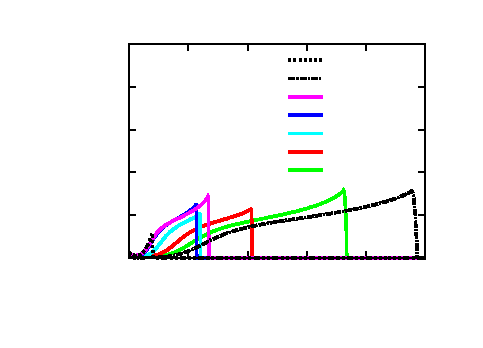
\includegraphics{ch-dynamics/H2O2_down_Z14}}%
    \gplfronttext
  \end{picture}%
\endgroup
}
  \resizebox{0.49\textwidth}{!}{% GNUPLOT: LaTeX picture with Postscript
\begingroup
  \makeatletter
  \providecommand\color[2][]{%
    \GenericError{(gnuplot) \space\space\space\@spaces}{%
      Package color not loaded in conjunction with
      terminal option `colourtext'%
    }{See the gnuplot documentation for explanation.%
    }{Either use 'blacktext' in gnuplot or load the package
      color.sty in LaTeX.}%
    \renewcommand\color[2][]{}%
  }%
  \providecommand\includegraphics[2][]{%
    \GenericError{(gnuplot) \space\space\space\@spaces}{%
      Package graphicx or graphics not loaded%
    }{See the gnuplot documentation for explanation.%
    }{The gnuplot epslatex terminal needs graphicx.sty or graphics.sty.}%
    \renewcommand\includegraphics[2][]{}%
  }%
  \providecommand\rotatebox[2]{#2}%
  \@ifundefined{ifGPcolor}{%
    \newif\ifGPcolor
    \GPcolortrue
  }{}%
  \@ifundefined{ifGPblacktext}{%
    \newif\ifGPblacktext
    \GPblacktexttrue
  }{}%
  % define a \g@addto@macro without @ in the name:
  \let\gplgaddtomacro\g@addto@macro
  % define empty templates for all commands taking text:
  \gdef\gplbacktext{}%
  \gdef\gplfronttext{}%
  \makeatother
  \ifGPblacktext
    % no textcolor at all
    \def\colorrgb#1{}%
    \def\colorgray#1{}%
  \else
    % gray or color?
    \ifGPcolor
      \def\colorrgb#1{\color[rgb]{#1}}%
      \def\colorgray#1{\color[gray]{#1}}%
      \expandafter\def\csname LTw\endcsname{\color{white}}%
      \expandafter\def\csname LTb\endcsname{\color{black}}%
      \expandafter\def\csname LTa\endcsname{\color{black}}%
      \expandafter\def\csname LT0\endcsname{\color[rgb]{1,0,0}}%
      \expandafter\def\csname LT1\endcsname{\color[rgb]{0,1,0}}%
      \expandafter\def\csname LT2\endcsname{\color[rgb]{0,0,1}}%
      \expandafter\def\csname LT3\endcsname{\color[rgb]{1,0,1}}%
      \expandafter\def\csname LT4\endcsname{\color[rgb]{0,1,1}}%
      \expandafter\def\csname LT5\endcsname{\color[rgb]{1,1,0}}%
      \expandafter\def\csname LT6\endcsname{\color[rgb]{0,0,0}}%
      \expandafter\def\csname LT7\endcsname{\color[rgb]{1,0.3,0}}%
      \expandafter\def\csname LT8\endcsname{\color[rgb]{0.5,0.5,0.5}}%
    \else
      % gray
      \def\colorrgb#1{\color{black}}%
      \def\colorgray#1{\color[gray]{#1}}%
      \expandafter\def\csname LTw\endcsname{\color{white}}%
      \expandafter\def\csname LTb\endcsname{\color{black}}%
      \expandafter\def\csname LTa\endcsname{\color{black}}%
      \expandafter\def\csname LT0\endcsname{\color{black}}%
      \expandafter\def\csname LT1\endcsname{\color{black}}%
      \expandafter\def\csname LT2\endcsname{\color{black}}%
      \expandafter\def\csname LT3\endcsname{\color{black}}%
      \expandafter\def\csname LT4\endcsname{\color{black}}%
      \expandafter\def\csname LT5\endcsname{\color{black}}%
      \expandafter\def\csname LT6\endcsname{\color{black}}%
      \expandafter\def\csname LT7\endcsname{\color{black}}%
      \expandafter\def\csname LT8\endcsname{\color{black}}%
    \fi
  \fi
  \setlength{\unitlength}{0.0500bp}%
  \begin{picture}(4320.00,3024.00)%
    \gplgaddtomacro\gplbacktext{%
      \csname LTb\endcsname%
      \put(948,704){\makebox(0,0)[r]{\strut{}0.0e+00}}%
      \put(948,1115){\makebox(0,0)[r]{\strut{}6.0e-03}}%
      \put(948,1526){\makebox(0,0)[r]{\strut{}1.2e-02}}%
      \put(948,1937){\makebox(0,0)[r]{\strut{}1.8e-02}}%
      \put(948,2348){\makebox(0,0)[r]{\strut{}2.4e-02}}%
      \put(948,2759){\makebox(0,0)[r]{\strut{}3.0e-02}}%
      \put(1080,484){\makebox(0,0){\strut{} 0}}%
      \put(1649,484){\makebox(0,0){\strut{} 2}}%
      \put(2217,484){\makebox(0,0){\strut{} 4}}%
      \put(2786,484){\makebox(0,0){\strut{} 6}}%
      \put(3354,484){\makebox(0,0){\strut{} 8}}%
      \put(3923,484){\makebox(0,0){\strut{} 10}}%
      \put(-218,1731){\rotatebox{-270}{\makebox(0,0){\strut{}\vspace{-28pt}$Y_{\rm H_2O_2}$}}}%
      \put(2501,154){\makebox(0,0){\strut{}$x/D$}}%
      \put(1506,2896){\makebox(0,0)[l]{\strut{}$Z = 0.24$ Decreasing-velocity Cycle}}%
    }%
    \gplgaddtomacro\gplfronttext{%
      \csname LTb\endcsname%
      \put(2763,1899){\makebox(0,0)[r]{\strut{}0.5 cycle}}%
      \csname LTb\endcsname%
      \put(2763,2075){\makebox(0,0)[r]{\strut{}0.45 cycle}}%
      \csname LTb\endcsname%
      \put(2763,2251){\makebox(0,0)[r]{\strut{}0.25 cycle}}%
      \csname LTb\endcsname%
      \put(2763,2427){\makebox(0,0)[r]{\strut{}Steady 8.0 m/s}}%
      \csname LTb\endcsname%
      \put(2763,2603){\makebox(0,0)[r]{\strut{}Steady 2.4 m/s}}%
    }%
    \gplbacktext
    \put(0,0){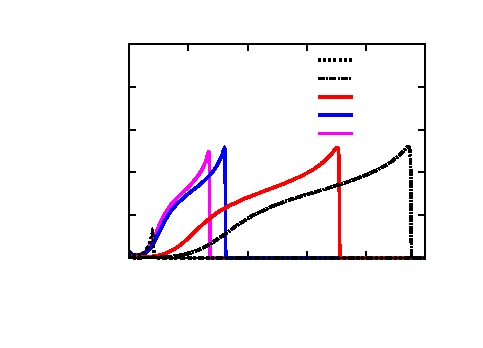
\includegraphics{ch-dynamics/H2O2_up_Z24}}%
    \gplfronttext
  \end{picture}%
\endgroup
}
  \resizebox{0.49\textwidth}{!}{% GNUPLOT: LaTeX picture with Postscript
\begingroup
  \makeatletter
  \providecommand\color[2][]{%
    \GenericError{(gnuplot) \space\space\space\@spaces}{%
      Package color not loaded in conjunction with
      terminal option `colourtext'%
    }{See the gnuplot documentation for explanation.%
    }{Either use 'blacktext' in gnuplot or load the package
      color.sty in LaTeX.}%
    \renewcommand\color[2][]{}%
  }%
  \providecommand\includegraphics[2][]{%
    \GenericError{(gnuplot) \space\space\space\@spaces}{%
      Package graphicx or graphics not loaded%
    }{See the gnuplot documentation for explanation.%
    }{The gnuplot epslatex terminal needs graphicx.sty or graphics.sty.}%
    \renewcommand\includegraphics[2][]{}%
  }%
  \providecommand\rotatebox[2]{#2}%
  \@ifundefined{ifGPcolor}{%
    \newif\ifGPcolor
    \GPcolortrue
  }{}%
  \@ifundefined{ifGPblacktext}{%
    \newif\ifGPblacktext
    \GPblacktexttrue
  }{}%
  % define a \g@addto@macro without @ in the name:
  \let\gplgaddtomacro\g@addto@macro
  % define empty templates for all commands taking text:
  \gdef\gplbacktext{}%
  \gdef\gplfronttext{}%
  \makeatother
  \ifGPblacktext
    % no textcolor at all
    \def\colorrgb#1{}%
    \def\colorgray#1{}%
  \else
    % gray or color?
    \ifGPcolor
      \def\colorrgb#1{\color[rgb]{#1}}%
      \def\colorgray#1{\color[gray]{#1}}%
      \expandafter\def\csname LTw\endcsname{\color{white}}%
      \expandafter\def\csname LTb\endcsname{\color{black}}%
      \expandafter\def\csname LTa\endcsname{\color{black}}%
      \expandafter\def\csname LT0\endcsname{\color[rgb]{1,0,0}}%
      \expandafter\def\csname LT1\endcsname{\color[rgb]{0,1,0}}%
      \expandafter\def\csname LT2\endcsname{\color[rgb]{0,0,1}}%
      \expandafter\def\csname LT3\endcsname{\color[rgb]{1,0,1}}%
      \expandafter\def\csname LT4\endcsname{\color[rgb]{0,1,1}}%
      \expandafter\def\csname LT5\endcsname{\color[rgb]{1,1,0}}%
      \expandafter\def\csname LT6\endcsname{\color[rgb]{0,0,0}}%
      \expandafter\def\csname LT7\endcsname{\color[rgb]{1,0.3,0}}%
      \expandafter\def\csname LT8\endcsname{\color[rgb]{0.5,0.5,0.5}}%
    \else
      % gray
      \def\colorrgb#1{\color{black}}%
      \def\colorgray#1{\color[gray]{#1}}%
      \expandafter\def\csname LTw\endcsname{\color{white}}%
      \expandafter\def\csname LTb\endcsname{\color{black}}%
      \expandafter\def\csname LTa\endcsname{\color{black}}%
      \expandafter\def\csname LT0\endcsname{\color{black}}%
      \expandafter\def\csname LT1\endcsname{\color{black}}%
      \expandafter\def\csname LT2\endcsname{\color{black}}%
      \expandafter\def\csname LT3\endcsname{\color{black}}%
      \expandafter\def\csname LT4\endcsname{\color{black}}%
      \expandafter\def\csname LT5\endcsname{\color{black}}%
      \expandafter\def\csname LT6\endcsname{\color{black}}%
      \expandafter\def\csname LT7\endcsname{\color{black}}%
      \expandafter\def\csname LT8\endcsname{\color{black}}%
    \fi
  \fi
  \setlength{\unitlength}{0.0500bp}%
  \begin{picture}(4320.00,3024.00)%
    \gplgaddtomacro\gplbacktext{%
      \csname LTb\endcsname%
      \put(948,704){\makebox(0,0)[r]{\strut{}0.0e+00}}%
      \put(948,1115){\makebox(0,0)[r]{\strut{}6.0e-03}}%
      \put(948,1526){\makebox(0,0)[r]{\strut{}1.2e-02}}%
      \put(948,1937){\makebox(0,0)[r]{\strut{}1.8e-02}}%
      \put(948,2348){\makebox(0,0)[r]{\strut{}2.4e-02}}%
      \put(948,2759){\makebox(0,0)[r]{\strut{}3.0e-02}}%
      \put(1080,484){\makebox(0,0){\strut{} 0}}%
      \put(1649,484){\makebox(0,0){\strut{} 2}}%
      \put(2217,484){\makebox(0,0){\strut{} 4}}%
      \put(2786,484){\makebox(0,0){\strut{} 6}}%
      \put(3354,484){\makebox(0,0){\strut{} 8}}%
      \put(3923,484){\makebox(0,0){\strut{} 10}}%
      \put(-218,1731){\rotatebox{-270}{\makebox(0,0){\strut{}\vspace{-28pt}$Y_{\rm H_2O_2}$}}}%
      \put(2501,154){\makebox(0,0){\strut{}$x/D$}}%
      \put(1506,2896){\makebox(0,0)[l]{\strut{}$Z = 0.24$ Increasing-velocity Cycle}}%
    }%
    \gplgaddtomacro\gplfronttext{%
      \csname LTb\endcsname%
      \put(2479,1547){\makebox(0,0)[r]{\strut{}0.85 cycle}}%
      \csname LTb\endcsname%
      \put(2479,1723){\makebox(0,0)[r]{\strut{}0.75 cycle}}%
      \csname LTb\endcsname%
      \put(2479,1899){\makebox(0,0)[r]{\strut{}0.65 cycle}}%
      \csname LTb\endcsname%
      \put(2479,2075){\makebox(0,0)[r]{\strut{}0.55 cycle}}%
      \csname LTb\endcsname%
      \put(2479,2251){\makebox(0,0)[r]{\strut{}0.5 cycle}}%
      \csname LTb\endcsname%
      \put(2479,2427){\makebox(0,0)[r]{\strut{}Steady 8.0 m/s}}%
      \csname LTb\endcsname%
      \put(2479,2603){\makebox(0,0)[r]{\strut{}Steady 2.4 m/s}}%
    }%
    \gplbacktext
    \put(0,0){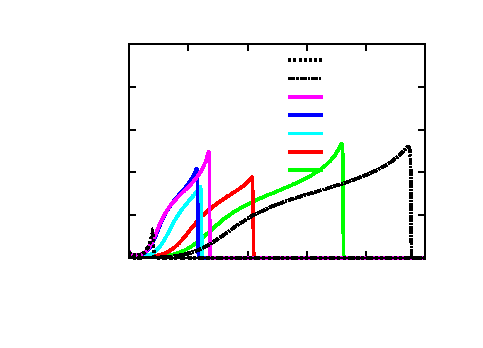
\includegraphics{H2O2_down_Z24}}%
    \gplfronttext
  \end{picture}%
\endgroup
}
  \normalsize
  \caption{Comparison of hydrogen peroxide mass fraction profiles along the $Z = 0.14$ and $Z = 0.24$ iso-contours at steady state and at $100$ Hz during the decreasing-velocity cycle (left) and increasing-velocity cycle (right).}
  \label{fig:H2O2_updown}
\end{figure}

As hydrogen peroxide plays different roles in the tribrachial flame and autoignition front, its spatial profiles along the $Z = 0.14$ and $Z = 0.24$ iso-contours are compared in Fig.~\ref{fig:H2O2_updown}, with the left and right subfigures corresponding to the decreasing-velocity and increasing-velocity half cycles, respectively.  Qualitatively, the evolution of the hydrogen peroxide profiles shows similar trends along both mixture fraction iso-contours.  The left figures show that hydrogen peroxide accumulates until either autoignition occurs or it is consumed at the flame front, resulting in a sharp drop in its mass fraction.  However, depending on the mixture fraction, the peak value of the hydrogen peroxide mass fraction differs by three to five times between a steady autoignition front (the steady 8.0 m/s case) and a tribrachial flame (the steady 2.4 m/s case), which implies its different significance in these two combustion modes and sets the benchmark for the unsteady evolution.  As the inlet velocity decreases from $8.0$ m/s, the peak $Y_{\rm H{_2}O{_2}}$ almost remains constant, indicating that the chemical structure is very close to the steady autoignition case.  As a consequence, the dominant chemical pathway remains H$_2$O$_2$ + M $\Longleftrightarrow$ OH + OH + M, and autoignition is the dominant combustion process, resulting in larger $S_d/S_L$.  However, as the flow velocity decreases, a larger gradient is achieved, resulting in steeper profiles and smaller $S_d/S_L$, according to Eq.~(\ref{eq:sd}).  The large gradient results in enhanced back diffusion from the reacting front to the unburnt upstream mixture and ultimately drives the transition into a tribrachial flame.

Even when the inlet velocity reaches the minimum $2.4$ m/s, which is the same as the steady case, the reacting front continues to move upstream.  Inlet velocity changes slowest around the half cycle, allowing the chemical structure to respond to the hydrodynamic changes.  As shown on the right of Fig.~\ref{fig:H2O2_updown}, the peak $Y_{\rm H{_2}O{_2}}$ decreases from $0.5$ to $0.65$ of the cycle.  At this stage, autoignition is not fully activated, since the peak $Y_{\rm H{_2}O{_2}}$ is lower than the steady autoignition case.  However, the peak $Y_{\rm H{_2}O{_2}}$ is still larger than the steady tribrachial flame.  Therefore, the $S_d/S_L$ of the tribrachial structure is close to but slightly larger than a steady flame, for it is propagating into a partially reacted mixture.  

As the inlet velocity further increases from $0.65$ to $0.75$ of the cycle, the propagation speed of the tribrachial flame cannot keep up with the flow incoming velocity, and the flame structure is therefore convected downstream.  During this flame blow-off process, $S_d/S_L$ remains essentially constant, which is demonstrated as the flattened bottom in Fig.~\ref{fig:sd_hys}.  Meanwhile, the unburnt mixture upstream of the flame accumulates radicals and heat as it moves downstream and eventually triggers autoignition, indicated by a sudden jump of $S_d/S_L$.  The time difference between the half cycle (where the inlet velocity is 2.4 m/s) and the last sample point before the sudden jump of $S_d/S_L$ is defined as the induction period, as indicated in Fig.~\ref{fig:sd_hys}.

\subsection{Effects of Oscillation Frequency} \label{sec:frq}

To better understand the coupling between hydrodynamics and chemistry and the hysteretic behavior in Fig.~\ref{fig:sd_hys}, the effects of oscillation frequency are analyzed.  Compared to the $100$ Hz case, the other two cases of lower oscillation frequency are similar qualitatively but with some quantitative differences.  Figure~\ref{fig:xd_evo} shows the evolution of the normalized leading point location ($x_d/D$) for the three oscillating cases, compared with the steady benchmark cases.  The peak-to-peak variation represents the oscillation amplitude during a cycle.  Two distinct trends are evident.  First, as the oscillation frequency increases, the oscillation amplitude decreases.  Extrapolating, if the oscillation frequency were much faster than any chemical or transport times scale, the oscillation amplitude would be zero, since the thermal structure could not respond to the velocity changes.

Second and more interestingly, for all three frequencies, the most downstream points during the oscillation are almost identical to the steady case at 8.0 m/s.  However, as the frequency increases, the most upstream point during the oscillation deviates more from the steady case at 2.4 m/s.  The different effects of oscillation frequency on the most downstream and upstream points are attributed to the difference in the combustion mode at these two locations.  As demonstrated in Fig.~\ref{fig:sd_hys}, the 100 Hz oscillating case has already established quasi-steady state when the boundary velocity is at 8.0 m/s when the combustion mode is kinetically controlled by autoignition.  In a Lagrangian sense, the location of an autoignition front is directly related to the ignition delay time, determined by chemical kinetics.  Therefore, the location of the autoignition front at this quasi-steady state is almost the same as the steady case with the same boundary velocity, which can be crudely estimated as the product of the ignition delay time and the boundary velocity.  For even lower frequency cases, such a quasi-steady state is even easier to achieve.  Consequently, for all three oscillation frequencies, the most downstream points remain very close to the steady autoignition governed case with the boundary velocity of 8.0 m/s.  Conversely, the stabilization mechanism for the steady case at 2.4 m/s is kinematically controlled by the balance between the tribrachial flame propagation speed and the incoming flow speed.  For the 100 Hz case, however, such kinematic balance never achieves quasi-steady state, as discussed in the previous section.  The location of the tribrachial flame is then determined kinematically both by the velocity difference between the unsteady tribrachial flame propagation speed and the flow speed and the time allowed for such displacement to occur.  At lower oscillation frequencies, longer time is allowed for the tribrachial flame to propagate upstream into the partially reacted mixture, while the displacement velocity decreases gradually due to reduced reactivity upstream.  The most upstream point location will then asymptotically approaches the steady state case when the oscillation frequency is sufficiently low.  This explains why the minimum $x_d/D$ approaches the steady state case at 2.4 m/s more closely at lower oscillation frequency in Fig.~\ref{fig:xd_evo}.

\begin{figure}[t]
  \centering
  \scriptsize
  \resizebox{1.0\textwidth}{!}{% GNUPLOT: LaTeX picture with Postscript
\begingroup
  \makeatletter
  \providecommand\color[2][]{%
    \GenericError{(gnuplot) \space\space\space\@spaces}{%
      Package color not loaded in conjunction with
      terminal option `colourtext'%
    }{See the gnuplot documentation for explanation.%
    }{Either use 'blacktext' in gnuplot or load the package
      color.sty in LaTeX.}%
    \renewcommand\color[2][]{}%
  }%
  \providecommand\includegraphics[2][]{%
    \GenericError{(gnuplot) \space\space\space\@spaces}{%
      Package graphicx or graphics not loaded%
    }{See the gnuplot documentation for explanation.%
    }{The gnuplot epslatex terminal needs graphicx.sty or graphics.sty.}%
    \renewcommand\includegraphics[2][]{}%
  }%
  \providecommand\rotatebox[2]{#2}%
  \@ifundefined{ifGPcolor}{%
    \newif\ifGPcolor
    \GPcolortrue
  }{}%
  \@ifundefined{ifGPblacktext}{%
    \newif\ifGPblacktext
    \GPblacktexttrue
  }{}%
  % define a \g@addto@macro without @ in the name:
  \let\gplgaddtomacro\g@addto@macro
  % define empty templates for all commands taking text:
  \gdef\gplbacktext{}%
  \gdef\gplfronttext{}%
  \makeatother
  \ifGPblacktext
    % no textcolor at all
    \def\colorrgb#1{}%
    \def\colorgray#1{}%
  \else
    % gray or color?
    \ifGPcolor
      \def\colorrgb#1{\color[rgb]{#1}}%
      \def\colorgray#1{\color[gray]{#1}}%
      \expandafter\def\csname LTw\endcsname{\color{white}}%
      \expandafter\def\csname LTb\endcsname{\color{black}}%
      \expandafter\def\csname LTa\endcsname{\color{black}}%
      \expandafter\def\csname LT0\endcsname{\color[rgb]{1,0,0}}%
      \expandafter\def\csname LT1\endcsname{\color[rgb]{0,1,0}}%
      \expandafter\def\csname LT2\endcsname{\color[rgb]{0,0,1}}%
      \expandafter\def\csname LT3\endcsname{\color[rgb]{1,0,1}}%
      \expandafter\def\csname LT4\endcsname{\color[rgb]{0,1,1}}%
      \expandafter\def\csname LT5\endcsname{\color[rgb]{1,1,0}}%
      \expandafter\def\csname LT6\endcsname{\color[rgb]{0,0,0}}%
      \expandafter\def\csname LT7\endcsname{\color[rgb]{1,0.3,0}}%
      \expandafter\def\csname LT8\endcsname{\color[rgb]{0.5,0.5,0.5}}%
    \else
      % gray
      \def\colorrgb#1{\color{black}}%
      \def\colorgray#1{\color[gray]{#1}}%
      \expandafter\def\csname LTw\endcsname{\color{white}}%
      \expandafter\def\csname LTb\endcsname{\color{black}}%
      \expandafter\def\csname LTa\endcsname{\color{black}}%
      \expandafter\def\csname LT0\endcsname{\color{black}}%
      \expandafter\def\csname LT1\endcsname{\color{black}}%
      \expandafter\def\csname LT2\endcsname{\color{black}}%
      \expandafter\def\csname LT3\endcsname{\color{black}}%
      \expandafter\def\csname LT4\endcsname{\color{black}}%
      \expandafter\def\csname LT5\endcsname{\color{black}}%
      \expandafter\def\csname LT6\endcsname{\color{black}}%
      \expandafter\def\csname LT7\endcsname{\color{black}}%
      \expandafter\def\csname LT8\endcsname{\color{black}}%
    \fi
  \fi
  \setlength{\unitlength}{0.0500bp}%
  \begin{picture}(5760.00,4032.00)%
    \gplgaddtomacro\gplbacktext{%
      \csname LTb\endcsname%
      \put(588,704){\makebox(0,0)[r]{\strut{} 0}}%
      \put(588,1317){\makebox(0,0)[r]{\strut{} 3}}%
      \put(588,1929){\makebox(0,0)[r]{\strut{} 6}}%
      \put(588,2542){\makebox(0,0)[r]{\strut{} 9}}%
      \put(588,3154){\makebox(0,0)[r]{\strut{} 12}}%
      \put(588,3767){\makebox(0,0)[r]{\strut{} 15}}%
      \put(720,484){\makebox(0,0){\strut{} 0}}%
      \put(1260,484){\makebox(0,0){\strut{} 0.25}}%
      \put(1800,484){\makebox(0,0){\strut{} 0.5}}%
      \put(2340,484){\makebox(0,0){\strut{} 0.75}}%
      \put(2880,484){\makebox(0,0){\strut{} 1}}%
      \put(3419,484){\makebox(0,0){\strut{} 1.25}}%
      \put(3959,484){\makebox(0,0){\strut{} 1.5}}%
      \put(4499,484){\makebox(0,0){\strut{} 1.75}}%
      \put(5039,484){\makebox(0,0){\strut{} 2}}%
      \put(-50,2235){\rotatebox{-270}{\makebox(0,0){\strut{}\vspace{-28pt}$x_d/D$}}}%
      \put(2879,154){\makebox(0,0){\strut{}Cycle}}%
    }%
    \gplgaddtomacro\gplfronttext{%
      \csname LTb\endcsname%
      \put(2068,3577){\makebox(0,0)[r]{\strut{}Steady 2.4 m/s}}%
      \csname LTb\endcsname%
      \put(2068,3401){\makebox(0,0)[r]{\strut{}Steady 8.0 m/s}}%
      \csname LTb\endcsname%
      \put(2068,3225){\makebox(0,0)[r]{\strut{}100 Hz}}%
      \csname LTb\endcsname%
      \put(2068,3049){\makebox(0,0)[r]{\strut{}50 Hz}}%
      \csname LTb\endcsname%
      \put(2068,2873){\makebox(0,0)[r]{\strut{}25 Hz}}%
    }%
    \gplbacktext
    \put(0,0){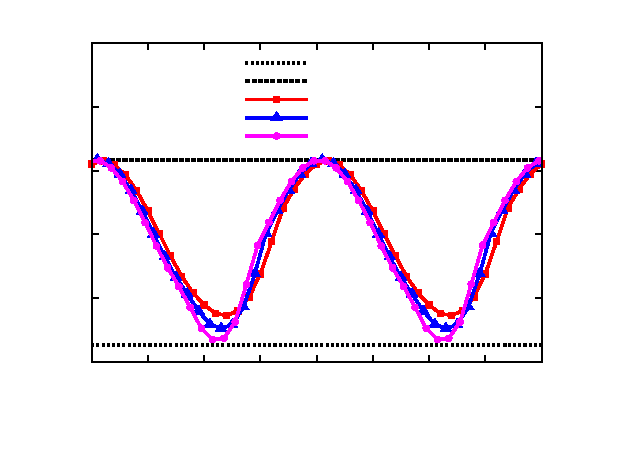
\includegraphics{xd_evo}}%
    \gplfronttext
  \end{picture}%
\endgroup
}
  \normalsize
  \caption{Normalized leading point location time history profiles at 25, 50, and 100 Hz.}
  \label{fig:xd_evo}
\end{figure}    

Besides the oscillation amplitude, the hysteretic behavior is also affected by the oscillation frequency.  As shown in Fig.~\ref{fig:sd_hys_frq}, the hysteresis of decreasing and increasing velocity is diminished as the oscillation frequency decreases, denoted by the shrinking of the enclosed area.  Hysteresis remains at slower inlet velocities since the decreasing-velocity branch is still autoignition dominated, but it takes finite induction time for the increasing-velocity unburnt mixture to achieve autoignition.  At higher inlet velocities, both branches are autoignition dominant and therefore collapse to a single path at sufficiently low frequency, approaching the quasi-steady limit.  Ideally, the quasi-steady limit could be achieved by investigating even lower frequencies, such as 0.1 Hz; however, such calculation would be extraordinarily intensive, requiring more than 20 million core-hours.  Instead, three steady state cases reported previously in Sec.~\ref{sec:dynamics-V} and a new steady case at the boundary velocity of 6.4 m/s are also included in Fig.~\ref{fig:sd_hys_frq} to illustrate the steady state limit.  The 3.2 m/s case is kinematically stabilized, similar to the 2.4 m/s case, and therefore is closer to the increasing-velocity branches of the oscillating cases but is different from the decreasing-velocity branches for the same reason at the lower velocity condition, as discussed in the previous section.  Conversely, the 6.4 m/s case is kinetically stabilized by autoignition, which can be approached by both the decreasing-velocity and increasing-velocity branches at lower oscillation frequency.

\begin{figure}[t]
  \centering
  \scriptsize
  \resizebox{1.0\textwidth}{!}{% GNUPLOT: LaTeX picture with Postscript
\begingroup
  \makeatletter
  \providecommand\color[2][]{%
    \GenericError{(gnuplot) \space\space\space\@spaces}{%
      Package color not loaded in conjunction with
      terminal option `colourtext'%
    }{See the gnuplot documentation for explanation.%
    }{Either use 'blacktext' in gnuplot or load the package
      color.sty in LaTeX.}%
    \renewcommand\color[2][]{}%
  }%
  \providecommand\includegraphics[2][]{%
    \GenericError{(gnuplot) \space\space\space\@spaces}{%
      Package graphicx or graphics not loaded%
    }{See the gnuplot documentation for explanation.%
    }{The gnuplot epslatex terminal needs graphicx.sty or graphics.sty.}%
    \renewcommand\includegraphics[2][]{}%
  }%
  \providecommand\rotatebox[2]{#2}%
  \@ifundefined{ifGPcolor}{%
    \newif\ifGPcolor
    \GPcolortrue
  }{}%
  \@ifundefined{ifGPblacktext}{%
    \newif\ifGPblacktext
    \GPblacktexttrue
  }{}%
  % define a \g@addto@macro without @ in the name:
  \let\gplgaddtomacro\g@addto@macro
  % define empty templates for all commands taking text:
  \gdef\gplbacktext{}%
  \gdef\gplfronttext{}%
  \makeatother
  \ifGPblacktext
    % no textcolor at all
    \def\colorrgb#1{}%
    \def\colorgray#1{}%
  \else
    % gray or color?
    \ifGPcolor
      \def\colorrgb#1{\color[rgb]{#1}}%
      \def\colorgray#1{\color[gray]{#1}}%
      \expandafter\def\csname LTw\endcsname{\color{white}}%
      \expandafter\def\csname LTb\endcsname{\color{black}}%
      \expandafter\def\csname LTa\endcsname{\color{black}}%
      \expandafter\def\csname LT0\endcsname{\color[rgb]{1,0,0}}%
      \expandafter\def\csname LT1\endcsname{\color[rgb]{0,1,0}}%
      \expandafter\def\csname LT2\endcsname{\color[rgb]{0,0,1}}%
      \expandafter\def\csname LT3\endcsname{\color[rgb]{1,0,1}}%
      \expandafter\def\csname LT4\endcsname{\color[rgb]{0,1,1}}%
      \expandafter\def\csname LT5\endcsname{\color[rgb]{1,1,0}}%
      \expandafter\def\csname LT6\endcsname{\color[rgb]{0,0,0}}%
      \expandafter\def\csname LT7\endcsname{\color[rgb]{1,0.3,0}}%
      \expandafter\def\csname LT8\endcsname{\color[rgb]{0.5,0.5,0.5}}%
    \else
      % gray
      \def\colorrgb#1{\color{black}}%
      \def\colorgray#1{\color[gray]{#1}}%
      \expandafter\def\csname LTw\endcsname{\color{white}}%
      \expandafter\def\csname LTb\endcsname{\color{black}}%
      \expandafter\def\csname LTa\endcsname{\color{black}}%
      \expandafter\def\csname LT0\endcsname{\color{black}}%
      \expandafter\def\csname LT1\endcsname{\color{black}}%
      \expandafter\def\csname LT2\endcsname{\color{black}}%
      \expandafter\def\csname LT3\endcsname{\color{black}}%
      \expandafter\def\csname LT4\endcsname{\color{black}}%
      \expandafter\def\csname LT5\endcsname{\color{black}}%
      \expandafter\def\csname LT6\endcsname{\color{black}}%
      \expandafter\def\csname LT7\endcsname{\color{black}}%
      \expandafter\def\csname LT8\endcsname{\color{black}}%
    \fi
  \fi
  \setlength{\unitlength}{0.0500bp}%
  \begin{picture}(5760.00,4032.00)%
    \gplgaddtomacro\gplbacktext{%
      \csname LTb\endcsname%
      \put(588,704){\makebox(0,0)[r]{\strut{} 0}}%
      \put(588,1317){\makebox(0,0)[r]{\strut{} 2}}%
      \put(588,1929){\makebox(0,0)[r]{\strut{} 4}}%
      \put(588,2542){\makebox(0,0)[r]{\strut{} 6}}%
      \put(588,3154){\makebox(0,0)[r]{\strut{} 8}}%
      \put(588,3767){\makebox(0,0)[r]{\strut{} 10}}%
      \put(720,484){\makebox(0,0){\strut{} 0}}%
      \put(1584,484){\makebox(0,0){\strut{} 2}}%
      \put(2448,484){\makebox(0,0){\strut{} 4}}%
      \put(3311,484){\makebox(0,0){\strut{} 6}}%
      \put(4175,484){\makebox(0,0){\strut{} 8}}%
      \put(5039,484){\makebox(0,0){\strut{} 10}}%
      \put(-50,2235){\rotatebox{-270}{\makebox(0,0){\strut{}\vspace{-28pt}$S_d/S_L$}}}%
      \put(2879,154){\makebox(0,0){\strut{}$U_{\rm inlet}$}}%
      \put(1066,2848){\makebox(0,0)[l]{\strut{}Decreasing-velocity}}%
      \put(3743,1470){\makebox(0,0)[l]{\strut{}Increasing-velocity}}%
    }%
    \gplgaddtomacro\gplfronttext{%
      \csname LTb\endcsname%
      \put(1377,3618){\makebox(0,0)[r]{\strut{}Steady}}%
      \csname LTb\endcsname%
      \put(1377,3442){\makebox(0,0)[r]{\strut{}100 Hz}}%
      \csname LTb\endcsname%
      \put(1377,3266){\makebox(0,0)[r]{\strut{}50 Hz}}%
      \csname LTb\endcsname%
      \put(1377,3090){\makebox(0,0)[r]{\strut{}25 Hz}}%
    }%
    \gplbacktext
    \put(0,0){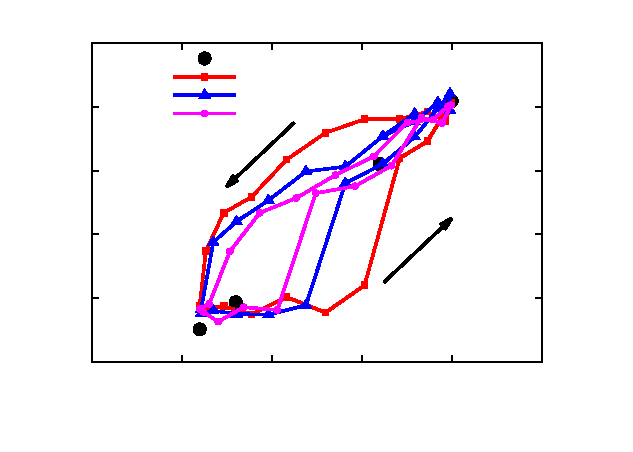
\includegraphics{sd_hys_frq}}%
    \gplfronttext
  \end{picture}%
\endgroup
}
  \normalsize
  \caption{Normalized displacement velocities at various inlet velocities for four steady cases and three oscillating unsteady cases at different frequencies.  Induction periods for the unsteady cases can also been defined similar to Fig.~\ref{fig:sd_hys} but are not shown here for clarity.}
  \label{fig:sd_hys_frq}
\end{figure}

In terms of the relative portion of the oscillation cycle, the 100 Hz case demonstrates a more pronounced hysteresis and longer induction period.  However, in term of the absolute time, shown in Table~\ref{table:ind}, the 25 Hz case takes a longer time to achieve the transition from small $S_d/S_L$ to larger values during the increasing-velocity portion of the cycle , noting that the time intervals between sampling points in Fig.~\ref{fig:sd_hys_frq} are not the same for the three frequencies, being $0.5$, $1.0$, and $2.0$ ms for 100, 50, and 25 Hz, respectively.

\begin{table*}
  \caption{Induction time at different harmonic oscillation frequencies.  The definition of the induction time is illustrated in Fig.~\ref{fig:sd_hys}}
  \label{table:ind}
  \centering
  \normalsize
  \resizebox{0.6\textwidth}{!}{
  \begin{tabular}{lc*{2}{c}}
    \hline
    Frequency [Hz]& $25$  & $50$  & $100$   \\
    \hline
    Induction Time [ms]& $6$ & $4$ & $2.5$\\
    \hline
   \end{tabular}
}
\end{table*}

This counter-intuitive finding is explained with Fig.~\ref{fig:ind_frq}.  Here, the temperature, hydrogen peroxide, and methoxymethylperoxy radical (CH$_3$OCH$_2$O$_2$) profiles are compared for the three frequency cases for both decreasing- and increasing-velocity branches at the same inlet velocity of $3.2$ m/s and benchmarked with the corresponding steady computation.  As in Secs.~\ref{sec:dynamics-T} and~\ref{sec:dynamics-V}, this steady case is autoignition dominated and stabilized at $Z = 0.24$.  

According to the temperature profiles, the steady and unsteady cases all demonstrate two heat release stages, with the first and second stage correlated well with the depletion of the CH$_3$OCH$_2$O$_2$ radical and hydrogen peroxide, respectively.  The CH$_3$OCH$_2$O$_2$ radical is often chosen to represent the NTC chemistry~\cite{krisman15}.  As demonstrated in the steady cases, NTC chemistry is important in the upstream of both tribrachial flame and autoignition front, and NTC chemistry is still important for the unsteady cases.  It is seen from Fig.~\ref{fig:ind_frq} that, irrespective of the oscillation frequency and traveling direction, at the same inlet velocity, $Y_{\rm CH_3OCH_2O_2}$ matches with its steady state profile, indicating that NTC chemistry responds to the flow oscillation relatively fast, and therefore is decoupled from flow dynamics.

Conversely, the coupling between fluid dynamics and second-stage autoignition/flame chemistry is important, for the hydrogen peroxide profiles of the unsteady cases fail to collapse onto that of the steady case.  Although three unsteady profiles on the decreasing-velocity branch show similar peak values, the lower the frequency, the closer the profile matches the steady case, which is expected from Fig.~\ref{fig:sd_hys_frq}.  However, the unsteady profiles on the increasing-velocity branch show lower peak values than the steady structure, with the $100$ Hz case profile being closer to the steady counterpart.  Noting from Fig.~\ref{fig:sd_hys_frq} that the minimum $S_d/S_L$ in all three cases are larger than the steady $2.4$ m/s case and at lower frequency the unburnt mixture has longer time to relax to steady state, the $25$ Hz case should match the $2.4$ m/s steady case closer, that is, a tribrachial flame with low H$_2$O$_2$ accumulation.  Therefore, a longer time is required to accumulate this lost H$_2$O$_2$ and activate autoignition.  Conversely, the $100$ Hz case allows less time to relax to a steady flame structure and therefore has larger $Y_{\rm H_2O_2}$ to start with during the increasing-velocity cycle, resulting in a shorter induction time for autoignition.

The different effects of oscillation frequency on the first-stage NTC chemistry and second-stage autoignition/flame chemistry can be understood by comparing the characteristic time scales of these processes.  The ignition delay time for the first-stage ignition facilitated by NTC chemistry is relatively short ($\sim$0.3 ms, according to Sec.~\ref{sec:dynamics-V}) compared to the major autoignition process induced by the hydrogen peroxide branching reaction ($\sim$1 ms, according to Sec.~\ref{sec:dynamics-V}) and the characteristic hydrodynamic oscillation time ($10$-$40$ ms in the unsteady cases).  Therefore, for the low frequency oscillations investigated in this section, the fluid dynamics and second-stage autoignition/flame chemistry coupling is mainly responsible for the hysteretic behavior and deviation from the steady state.

At even higher oscillation frequencies, the NTC chemistry could interact with the hydrodynamics.  Such conditions were attempted computationally, but the elevated frequency resulted in vortex shedding and local flame extinction, which add further complexity.

\begin{figure}[t]
  \centering
  \scriptsize
  \resizebox{0.8\textwidth}{!}{% GNUPLOT: LaTeX picture with Postscript
\begingroup
  \makeatletter
  \providecommand\color[2][]{%
    \GenericError{(gnuplot) \space\space\space\@spaces}{%
      Package color not loaded in conjunction with
      terminal option `colourtext'%
    }{See the gnuplot documentation for explanation.%
    }{Either use 'blacktext' in gnuplot or load the package
      color.sty in LaTeX.}%
    \renewcommand\color[2][]{}%
  }%
  \providecommand\includegraphics[2][]{%
    \GenericError{(gnuplot) \space\space\space\@spaces}{%
      Package graphicx or graphics not loaded%
    }{See the gnuplot documentation for explanation.%
    }{The gnuplot epslatex terminal needs graphicx.sty or graphics.sty.}%
    \renewcommand\includegraphics[2][]{}%
  }%
  \providecommand\rotatebox[2]{#2}%
  \@ifundefined{ifGPcolor}{%
    \newif\ifGPcolor
    \GPcolortrue
  }{}%
  \@ifundefined{ifGPblacktext}{%
    \newif\ifGPblacktext
    \GPblacktexttrue
  }{}%
  % define a \g@addto@macro without @ in the name:
  \let\gplgaddtomacro\g@addto@macro
  % define empty templates for all commands taking text:
  \gdef\gplbacktext{}%
  \gdef\gplfronttext{}%
  \makeatother
  \ifGPblacktext
    % no textcolor at all
    \def\colorrgb#1{}%
    \def\colorgray#1{}%
  \else
    % gray or color?
    \ifGPcolor
      \def\colorrgb#1{\color[rgb]{#1}}%
      \def\colorgray#1{\color[gray]{#1}}%
      \expandafter\def\csname LTw\endcsname{\color{white}}%
      \expandafter\def\csname LTb\endcsname{\color{black}}%
      \expandafter\def\csname LTa\endcsname{\color{black}}%
      \expandafter\def\csname LT0\endcsname{\color[rgb]{1,0,0}}%
      \expandafter\def\csname LT1\endcsname{\color[rgb]{0,1,0}}%
      \expandafter\def\csname LT2\endcsname{\color[rgb]{0,0,1}}%
      \expandafter\def\csname LT3\endcsname{\color[rgb]{1,0,1}}%
      \expandafter\def\csname LT4\endcsname{\color[rgb]{0,1,1}}%
      \expandafter\def\csname LT5\endcsname{\color[rgb]{1,1,0}}%
      \expandafter\def\csname LT6\endcsname{\color[rgb]{0,0,0}}%
      \expandafter\def\csname LT7\endcsname{\color[rgb]{1,0.3,0}}%
      \expandafter\def\csname LT8\endcsname{\color[rgb]{0.5,0.5,0.5}}%
    \else
      % gray
      \def\colorrgb#1{\color{black}}%
      \def\colorgray#1{\color[gray]{#1}}%
      \expandafter\def\csname LTw\endcsname{\color{white}}%
      \expandafter\def\csname LTb\endcsname{\color{black}}%
      \expandafter\def\csname LTa\endcsname{\color{black}}%
      \expandafter\def\csname LT0\endcsname{\color{black}}%
      \expandafter\def\csname LT1\endcsname{\color{black}}%
      \expandafter\def\csname LT2\endcsname{\color{black}}%
      \expandafter\def\csname LT3\endcsname{\color{black}}%
      \expandafter\def\csname LT4\endcsname{\color{black}}%
      \expandafter\def\csname LT5\endcsname{\color{black}}%
      \expandafter\def\csname LT6\endcsname{\color{black}}%
      \expandafter\def\csname LT7\endcsname{\color{black}}%
      \expandafter\def\csname LT8\endcsname{\color{black}}%
    \fi
  \fi
  \setlength{\unitlength}{0.0500bp}%
  \begin{picture}(5760.00,3024.00)%
    \gplgaddtomacro\gplbacktext{%
      \csname LTb\endcsname%
      \put(948,704){\makebox(0,0)[r]{\strut{}5.0e+02}}%
      \put(948,1115){\makebox(0,0)[r]{\strut{}9.0e+02}}%
      \put(948,1526){\makebox(0,0)[r]{\strut{}1.3e+03}}%
      \put(948,1937){\makebox(0,0)[r]{\strut{}1.7e+03}}%
      \put(948,2348){\makebox(0,0)[r]{\strut{}2.1e+03}}%
      \put(948,2759){\makebox(0,0)[r]{\strut{}2.5e+03}}%
      \put(1080,484){\makebox(0,0){\strut{} 0}}%
      \put(1937,484){\makebox(0,0){\strut{} 1}}%
      \put(2793,484){\makebox(0,0){\strut{} 2}}%
      \put(3650,484){\makebox(0,0){\strut{} 3}}%
      \put(4506,484){\makebox(0,0){\strut{} 4}}%
      \put(5363,484){\makebox(0,0){\strut{} 5}}%
      \put(-218,1731){\rotatebox{-270}{\makebox(0,0){\strut{}\vspace{-28pt}$T [K]$}}}%
      \put(3221,154){\makebox(0,0){\strut{}$x/D$}}%
    }%
    \gplgaddtomacro\gplfronttext{%
      \csname LTb\endcsname%
      \put(1966,2546){\makebox(0,0)[r]{\strut{}Steady 3.2 m/s}}%
      \csname LTb\endcsname%
      \put(1966,2326){\makebox(0,0)[r]{\strut{}100 Hz DV}}%
      \csname LTb\endcsname%
      \put(1966,2106){\makebox(0,0)[r]{\strut{}50 Hz DV}}%
      \csname LTb\endcsname%
      \put(1966,1886){\makebox(0,0)[r]{\strut{}25 Hz DV}}%
      \csname LTb\endcsname%
      \put(1966,1666){\makebox(0,0)[r]{\strut{}100 Hz IV}}%
      \csname LTb\endcsname%
      \put(1966,1446){\makebox(0,0)[r]{\strut{}50 Hz IV}}%
      \csname LTb\endcsname%
      \put(1966,1226){\makebox(0,0)[r]{\strut{}25 Hz IV}}%
    }%
    \gplbacktext
    \put(0,0){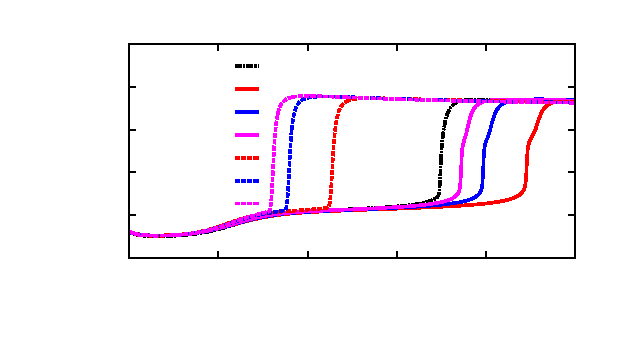
\includegraphics{ch-dynamics/T_32}}%
    \gplfronttext
  \end{picture}%
\endgroup
}
  \resizebox{0.8\textwidth}{!}{% GNUPLOT: LaTeX picture with Postscript
\begingroup
  \makeatletter
  \providecommand\color[2][]{%
    \GenericError{(gnuplot) \space\space\space\@spaces}{%
      Package color not loaded in conjunction with
      terminal option `colourtext'%
    }{See the gnuplot documentation for explanation.%
    }{Either use 'blacktext' in gnuplot or load the package
      color.sty in LaTeX.}%
    \renewcommand\color[2][]{}%
  }%
  \providecommand\includegraphics[2][]{%
    \GenericError{(gnuplot) \space\space\space\@spaces}{%
      Package graphicx or graphics not loaded%
    }{See the gnuplot documentation for explanation.%
    }{The gnuplot epslatex terminal needs graphicx.sty or graphics.sty.}%
    \renewcommand\includegraphics[2][]{}%
  }%
  \providecommand\rotatebox[2]{#2}%
  \@ifundefined{ifGPcolor}{%
    \newif\ifGPcolor
    \GPcolortrue
  }{}%
  \@ifundefined{ifGPblacktext}{%
    \newif\ifGPblacktext
    \GPblacktexttrue
  }{}%
  % define a \g@addto@macro without @ in the name:
  \let\gplgaddtomacro\g@addto@macro
  % define empty templates for all commands taking text:
  \gdef\gplbacktext{}%
  \gdef\gplfronttext{}%
  \makeatother
  \ifGPblacktext
    % no textcolor at all
    \def\colorrgb#1{}%
    \def\colorgray#1{}%
  \else
    % gray or color?
    \ifGPcolor
      \def\colorrgb#1{\color[rgb]{#1}}%
      \def\colorgray#1{\color[gray]{#1}}%
      \expandafter\def\csname LTw\endcsname{\color{white}}%
      \expandafter\def\csname LTb\endcsname{\color{black}}%
      \expandafter\def\csname LTa\endcsname{\color{black}}%
      \expandafter\def\csname LT0\endcsname{\color[rgb]{1,0,0}}%
      \expandafter\def\csname LT1\endcsname{\color[rgb]{0,1,0}}%
      \expandafter\def\csname LT2\endcsname{\color[rgb]{0,0,1}}%
      \expandafter\def\csname LT3\endcsname{\color[rgb]{1,0,1}}%
      \expandafter\def\csname LT4\endcsname{\color[rgb]{0,1,1}}%
      \expandafter\def\csname LT5\endcsname{\color[rgb]{1,1,0}}%
      \expandafter\def\csname LT6\endcsname{\color[rgb]{0,0,0}}%
      \expandafter\def\csname LT7\endcsname{\color[rgb]{1,0.3,0}}%
      \expandafter\def\csname LT8\endcsname{\color[rgb]{0.5,0.5,0.5}}%
    \else
      % gray
      \def\colorrgb#1{\color{black}}%
      \def\colorgray#1{\color[gray]{#1}}%
      \expandafter\def\csname LTw\endcsname{\color{white}}%
      \expandafter\def\csname LTb\endcsname{\color{black}}%
      \expandafter\def\csname LTa\endcsname{\color{black}}%
      \expandafter\def\csname LT0\endcsname{\color{black}}%
      \expandafter\def\csname LT1\endcsname{\color{black}}%
      \expandafter\def\csname LT2\endcsname{\color{black}}%
      \expandafter\def\csname LT3\endcsname{\color{black}}%
      \expandafter\def\csname LT4\endcsname{\color{black}}%
      \expandafter\def\csname LT5\endcsname{\color{black}}%
      \expandafter\def\csname LT6\endcsname{\color{black}}%
      \expandafter\def\csname LT7\endcsname{\color{black}}%
      \expandafter\def\csname LT8\endcsname{\color{black}}%
    \fi
  \fi
  \setlength{\unitlength}{0.0500bp}%
  \begin{picture}(5760.00,3024.00)%
    \gplgaddtomacro\gplbacktext{%
      \csname LTb\endcsname%
      \put(948,704){\makebox(0,0)[r]{\strut{}0.0e+00}}%
      \put(948,1115){\makebox(0,0)[r]{\strut{}7.0e-04}}%
      \put(948,1526){\makebox(0,0)[r]{\strut{}1.4e-03}}%
      \put(948,1937){\makebox(0,0)[r]{\strut{}2.1e-03}}%
      \put(948,2348){\makebox(0,0)[r]{\strut{}2.8e-03}}%
      \put(948,2759){\makebox(0,0)[r]{\strut{}3.5e-03}}%
      \put(1080,484){\makebox(0,0){\strut{} 0}}%
      \put(1937,484){\makebox(0,0){\strut{} 1}}%
      \put(2793,484){\makebox(0,0){\strut{} 2}}%
      \put(3650,484){\makebox(0,0){\strut{} 3}}%
      \put(4506,484){\makebox(0,0){\strut{} 4}}%
      \put(5363,484){\makebox(0,0){\strut{} 5}}%
      \put(-218,1731){\rotatebox{-270}{\makebox(0,0){\strut{}\vspace{-28pt}$Y_{\rm CH_3OCH_2O_2}$}}}%
      \put(3221,154){\makebox(0,0){\strut{}$x/D$}}%
    }%
    \gplgaddtomacro\gplfronttext{%
      \csname LTb\endcsname%
      \put(4707,2473){\makebox(0,0)[r]{\strut{}Steady 3.2 m/s}}%
      \csname LTb\endcsname%
      \put(4707,2253){\makebox(0,0)[r]{\strut{}100 Hz DV}}%
      \csname LTb\endcsname%
      \put(4707,2033){\makebox(0,0)[r]{\strut{}50 Hz DV}}%
      \csname LTb\endcsname%
      \put(4707,1813){\makebox(0,0)[r]{\strut{}25 Hz DV}}%
      \csname LTb\endcsname%
      \put(4707,1593){\makebox(0,0)[r]{\strut{}100 Hz IV}}%
      \csname LTb\endcsname%
      \put(4707,1373){\makebox(0,0)[r]{\strut{}50 Hz IV}}%
      \csname LTb\endcsname%
      \put(4707,1153){\makebox(0,0)[r]{\strut{}25 Hz IV}}%
    }%
    \gplbacktext
    \put(0,0){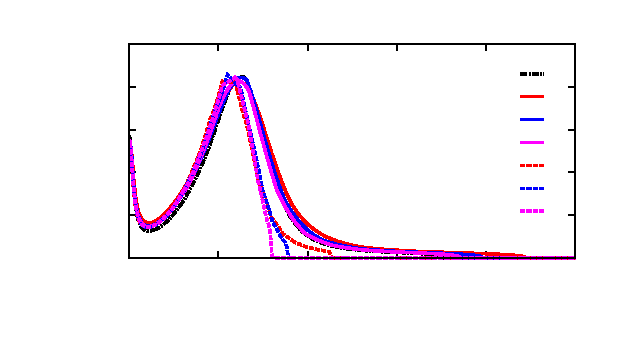
\includegraphics{RO2_32}}%
    \gplfronttext
  \end{picture}%
\endgroup
}
  \resizebox{0.8\textwidth}{!}{% GNUPLOT: LaTeX picture with Postscript
\begingroup
  \makeatletter
  \providecommand\color[2][]{%
    \GenericError{(gnuplot) \space\space\space\@spaces}{%
      Package color not loaded in conjunction with
      terminal option `colourtext'%
    }{See the gnuplot documentation for explanation.%
    }{Either use 'blacktext' in gnuplot or load the package
      color.sty in LaTeX.}%
    \renewcommand\color[2][]{}%
  }%
  \providecommand\includegraphics[2][]{%
    \GenericError{(gnuplot) \space\space\space\@spaces}{%
      Package graphicx or graphics not loaded%
    }{See the gnuplot documentation for explanation.%
    }{The gnuplot epslatex terminal needs graphicx.sty or graphics.sty.}%
    \renewcommand\includegraphics[2][]{}%
  }%
  \providecommand\rotatebox[2]{#2}%
  \@ifundefined{ifGPcolor}{%
    \newif\ifGPcolor
    \GPcolortrue
  }{}%
  \@ifundefined{ifGPblacktext}{%
    \newif\ifGPblacktext
    \GPblacktexttrue
  }{}%
  % define a \g@addto@macro without @ in the name:
  \let\gplgaddtomacro\g@addto@macro
  % define empty templates for all commands taking text:
  \gdef\gplbacktext{}%
  \gdef\gplfronttext{}%
  \makeatother
  \ifGPblacktext
    % no textcolor at all
    \def\colorrgb#1{}%
    \def\colorgray#1{}%
  \else
    % gray or color?
    \ifGPcolor
      \def\colorrgb#1{\color[rgb]{#1}}%
      \def\colorgray#1{\color[gray]{#1}}%
      \expandafter\def\csname LTw\endcsname{\color{white}}%
      \expandafter\def\csname LTb\endcsname{\color{black}}%
      \expandafter\def\csname LTa\endcsname{\color{black}}%
      \expandafter\def\csname LT0\endcsname{\color[rgb]{1,0,0}}%
      \expandafter\def\csname LT1\endcsname{\color[rgb]{0,1,0}}%
      \expandafter\def\csname LT2\endcsname{\color[rgb]{0,0,1}}%
      \expandafter\def\csname LT3\endcsname{\color[rgb]{1,0,1}}%
      \expandafter\def\csname LT4\endcsname{\color[rgb]{0,1,1}}%
      \expandafter\def\csname LT5\endcsname{\color[rgb]{1,1,0}}%
      \expandafter\def\csname LT6\endcsname{\color[rgb]{0,0,0}}%
      \expandafter\def\csname LT7\endcsname{\color[rgb]{1,0.3,0}}%
      \expandafter\def\csname LT8\endcsname{\color[rgb]{0.5,0.5,0.5}}%
    \else
      % gray
      \def\colorrgb#1{\color{black}}%
      \def\colorgray#1{\color[gray]{#1}}%
      \expandafter\def\csname LTw\endcsname{\color{white}}%
      \expandafter\def\csname LTb\endcsname{\color{black}}%
      \expandafter\def\csname LTa\endcsname{\color{black}}%
      \expandafter\def\csname LT0\endcsname{\color{black}}%
      \expandafter\def\csname LT1\endcsname{\color{black}}%
      \expandafter\def\csname LT2\endcsname{\color{black}}%
      \expandafter\def\csname LT3\endcsname{\color{black}}%
      \expandafter\def\csname LT4\endcsname{\color{black}}%
      \expandafter\def\csname LT5\endcsname{\color{black}}%
      \expandafter\def\csname LT6\endcsname{\color{black}}%
      \expandafter\def\csname LT7\endcsname{\color{black}}%
      \expandafter\def\csname LT8\endcsname{\color{black}}%
    \fi
  \fi
  \setlength{\unitlength}{0.0500bp}%
  \begin{picture}(4320.00,3024.00)%
    \gplgaddtomacro\gplbacktext{%
      \csname LTb\endcsname%
      \put(948,704){\makebox(0,0)[r]{\strut{}0.0e+00}}%
      \put(948,1115){\makebox(0,0)[r]{\strut{}6.0e-03}}%
      \put(948,1526){\makebox(0,0)[r]{\strut{}1.2e-02}}%
      \put(948,1937){\makebox(0,0)[r]{\strut{}1.8e-02}}%
      \put(948,2348){\makebox(0,0)[r]{\strut{}2.4e-02}}%
      \put(948,2759){\makebox(0,0)[r]{\strut{}3.0e-02}}%
      \put(1080,484){\makebox(0,0){\strut{} 0}}%
      \put(1649,484){\makebox(0,0){\strut{} 1}}%
      \put(2217,484){\makebox(0,0){\strut{} 2}}%
      \put(2786,484){\makebox(0,0){\strut{} 3}}%
      \put(3354,484){\makebox(0,0){\strut{} 4}}%
      \put(3923,484){\makebox(0,0){\strut{} 5}}%
      \put(-218,1731){\rotatebox{-270}{\makebox(0,0){\strut{}\vspace{-28pt}$Y_{\rm H_2O_2}$}}}%
      \put(2501,154){\makebox(0,0){\strut{}$x/D$}}%
    }%
    \gplgaddtomacro\gplfronttext{%
      \csname LTb\endcsname%
      \put(1960,2603){\makebox(0,0)[r]{\strut{}Steady 3.2 m/s}}%
      \csname LTb\endcsname%
      \put(1960,2427){\makebox(0,0)[r]{\strut{}100 Hz DV}}%
      \csname LTb\endcsname%
      \put(1960,2251){\makebox(0,0)[r]{\strut{}50 Hz DV}}%
      \csname LTb\endcsname%
      \put(1960,2075){\makebox(0,0)[r]{\strut{}25 Hz DV}}%
      \csname LTb\endcsname%
      \put(1960,1899){\makebox(0,0)[r]{\strut{}100 Hz IV}}%
      \csname LTb\endcsname%
      \put(1960,1723){\makebox(0,0)[r]{\strut{}50 Hz IV}}%
      \csname LTb\endcsname%
      \put(1960,1547){\makebox(0,0)[r]{\strut{}25 Hz IV}}%
    }%
    \gplbacktext
    \put(0,0){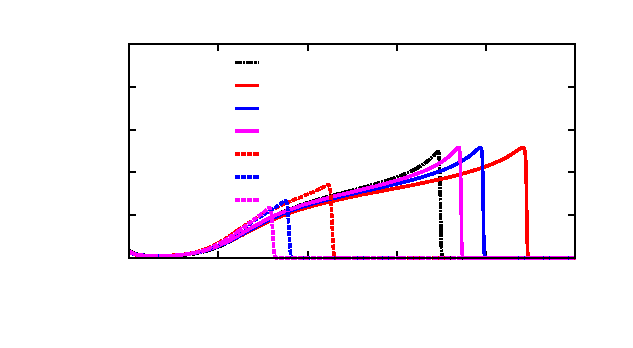
\includegraphics{H2O2_32}}%
    \gplfronttext
  \end{picture}%
\endgroup
}
  \normalsize
  \caption{Temperature, methyoxymethylperoxy radical, and hydrogen peroxide mass fraction profiles along the $Z = 0.24$ iso-contour at $3.2$ m/s.  DV: decreasing-velocity, and IV: increasing-velocity.}
  \label{fig:ind_frq}
\end{figure}

\section{Summary}

In this chapter, the two-dimensional nonpremixed DME flames in heated air coflows were investigated computationally due to the difficulty in well-controlled experiments otherwise.  The understanding of the low-temperature chemistry obtained in the one-dimensional counterflow configuration presented in Chapter~\ref{ch:NTC} is benefical to elucidate the importance of low-temperature chemistry in flame dynamics at elevated temperatures and pressures.  In the steady cases, besides the kinematic stabilization mechanism that balances the traditional tribrachial flame propagation in coflows at nonautoignitive conditions, the kinetic stabilization mechanism induced by autoignition can also be important under certain conditions.  Since low-temperature chemistry dictates the first-stage autoignition delay time and the subsequent heat release, it affects the morphology of the multibrachial structure of the autoignition front.  With advanced computational diagnostics, the thermal and chemical structures as well as the donimant stablization mechanisms were elucidated for steady cases at various boundary conditions.  A regime diagram was proposed to generalize the stablization mechanism.  

Furthermore, realizing that one of the major characteristics of practical engine conditions is unsteadiness, flame dynamics in the same configuration were investigated by forcing harmonic oscillations between two steady cases at different oscillation frequencies.  The transition in the combustion mode during the oscillation was observed and quantified.  Finally, the coupling effects of low-temperature chemistry, high-temperature chemistry, and transport were elucidated.  Such understanding could be benefical to future turbulent studies.
